\documentclass[a4paper,12pt]{article}

% ----------------------------
% Pacchetti utili
% ----------------------------
\usepackage[utf8]{inputenc}
\usepackage[T1]{fontenc}
\usepackage[italian]{babel}
\usepackage{graphicx}
\usepackage{tabularx}
\usepackage[table]{xcolor}
\definecolor{lightblue}{RGB}{225,240,255}
\definecolor{gold}{RGB}{255,215,0}
\usepackage{geometry}
\usepackage{setspace}
\usepackage{calc}
\usepackage{array}
\usepackage{fancyhdr}
\usepackage{comment}
\usepackage{tikz}
\usepackage{float}
\usepackage{xurl}
\usepackage{amsmath}
\usepackage{pgf-pie}
\usepackage{longtable}
\usepackage[colorlinks=true, linkcolor=blue, urlcolor=blue, citecolor=blue]{hyperref}
\usepackage{pgffor}
\usepackage{titlesec}

% Modifica la spaziatura di \subparagraph
% Argomenti: {comando} {rientro_sinistro} {spazio_sopra} {spazio_dopo}
\titlespacing*{\subparagraph}
{0pt}{3.25ex plus 1ex minus .2ex}{1em}

% ----------------------------
% Impostazioni pagina
% ----------------------------
\geometry{
    top=2cm,
    bottom=2cm,
    left=2cm,
    right=2cm
}

\setstretch{1.2}

% ----------------------------
% Dati personalizzabili
% ----------------------------
\newcommand{\Gruppo}{Atlas}
\newcommand{\Email}{\href{mailto:team9.atlas@gmail.com}{\textcolor{blue}{\underline{team9.atlas@gmail.com}}}}
\newcommand{\TitoloDocumento}{Specifica Tecnica}
\newcommand{\DataUltimaModifica}{2026/04/08}
\newcommand{\LogoGruppo}{../../../Assets/AtlasLogo.png}

% --- Nuove variabili aggiunte ---
\newcommand{\VersioneDocumento}{1.0.0}
\newcommand{\TipoDocumento}{Esterno} 

\pagestyle{fancy}
\fancyhf{}
\fancyhead[L]{\Gruppo}
\fancyhead[R]{Documento: \TipoDocumento}
\fancyfoot[C]{\thepage}

% larghezza della colonna dei nomi
\newlength{\namecol}
\setlength{\namecol}{4.5cm}
\setlength{\headheight}{15pt} % messo per evitare warning di fancyhdr


\newlength{\colw}
\setlength{\colw}{1.5cm}

\setcounter{secnumdepth}{5}
\setcounter{tocdepth}{5}

\definecolor{mioverde}{RGB}{20,150,60}

% ----------------------------
% Inizio documento
% ----------------------------
\begin{document}

% ----------------------------
% Prima pagina
% ----------------------------
\begin{titlepage}

    \begin{center}

        % Logo
        \vspace*{0cm}
        \begin{tikzpicture}
            \clip (0,-0.1) circle (5.6cm);
            \node at (0,0) {\includegraphics[width=12cm]{\LogoGruppo}};
        \end{tikzpicture}\\[0.8cm]

        % Barra superiore
        \noindent\rule{\textwidth}{0.4pt}

        % Titolo
        \vspace{1cm}
        {\Huge \textbf{\TitoloDocumento}}\\[0.4cm]
        {\large Progetto di Ingegneria del Software A.A. 2025/2026}\\[0.8cm]
        {\large Versione: \VersioneDocumento}
        \vspace{1cm}

        % Barra inferiore
        \noindent\rule{\textwidth}{0.4pt}

    \end{center}

    % Informazioni in basso
    \vfill
    \noindent
    \begin{minipage}{0.5\textwidth}
        \raggedright
        \textbf{Autore:} \Gruppo\\
        \textbf{Ultima modifica:} \DataUltimaModifica
    \end{minipage}%
    \begin{minipage}{0.5\textwidth}
        \raggedleft
        \textbf{Tipo di documento:} \TipoDocumento
    \end{minipage}

\end{titlepage}



\section*{Registro delle modifiche}
\begin{center}
    \rowcolors{2}{lightblue}{white}
    \begin{tabularx}{\textwidth}{|l|l|l|X|X|}
        \hline
        \rowcolor{lightgray}
        \textbf{Versione}  & \textbf{Data}       & \textbf{Autore}      & \textbf{Verificatore} & \textbf{Descrizione} \\
        \hline
        v1.0.0 & 2026/04/09 & Giacomo Giora & Michele Tesser & Approvazione documento \\
        \hline
        v0.8.0 & 2026/04/02 & Andrea Difino & Michele Tesser & Aggiunta design patterns \\
        \hline
        v0.7.3 & 2026/03/26 & Andrea Difino & Michele Tesser & Fine stesura frontend\\
        \hline
        v0.7.2 & 2026/03/24 & Andrea Difino & Michele Tesser & Aggiunta immagini\\
        \hline
        v0.7.1 & 2026/03/21 & Giacomo Giora & Federico Simonetto & Fine stesura elementi frontend\\
        \hline
        v0.7.0 & 2026/03/20 & Giacomo Giora & Federico Simonetto & Inizio stesura elementi frontend\\
        \hline
        v0.6.1 & 2026/03/19 & Giacomo Giora & Federico Simonetto & Fine stesura classi backend\\
        \hline
        v0.6.0 & 2026/03/16 & Giacomo Giora & Federico Simonetto & Inizio stesura architettura frontend\\
        \hline
        v0.5.1 & 2026/03/14 & Michele Tesser & Federico Simonetto & Fine stesura architettura\\
        \hline
        v0.5.0 & 2026/03/10 & Michele Tesser & Federico Simonetto & Inizio stesura classi backend \\
        \hline
        v0.4.0 & 2026/03/09 & Francesco Marcolongo & Federico Simonetto & Inizio stesura architettura \\
        \hline
        v0.3.1 & 2026/03/09 & Giacomo Giora & Federico Simonetto & Fine stesura tecnologie \\
        \hline
        v0.3.0 & 2026/03/08 & Giacomo Giora & Federico Simonetto & Inizio stesura tecnologie \\
        \hline
        v0.2.0 & 2026/03/07 & Federico Simonetto & Giacomo Giora & Stesura descrizione prodotto \\
        \hline
        v0.1.1 & 2026/03/06 & Federico Simonetto & Giacomo Giora & Aggiunti link ai riferimenti \\
        \hline
        v0.1.0 & 2026/03/05 & Federico Simonetto & Giacomo Giora & Prima stesura documento \\
        \hline
    \end{tabularx}
\end{center}

\newpage

\tableofcontents

%\newpage

%\listoffigures

%\newpage

%\listoftables

\newpage
% ----------------------------
% Inizio contenuto
% ----------------------------
\section{Introduzione}

    \subsection{Scopo del documento}
        Il presente documento ha l'\textit{obiettivo}\textsubscript{\href{https://atlasteam9.github.io/Atlas/glossario.html\#Obiettivo}{G}} di descrivere in maniera approfondita l'\textit{architettura}\textsubscript{\href{https://atlasteam9.github.io/Atlas/glossario.html\#Architettura}{G}} del prodotto software sviluppato dal team.
        In particolare, verranno presentati e analizzati i seguenti aspetti:
        \begin{itemize}
            \item le tecnologie selezionate per lo \textit{sviluppo}\textsubscript{\href{https://atlasteam9.github.io/Atlas/glossario.html\#Sviluppo}{G}} e per le attività di testing del prodotto;
            \item l'\textit{architettura}\textsubscript{\href{https://atlasteam9.github.io/Atlas/glossario.html\#Architettura}{G}} logica del sistema, con la descrizione dei principali moduli che lo compongono e delle interazioni tra di essi;
            \item l'\textit{architettura}\textsubscript{\href{https://atlasteam9.github.io/Atlas/glossario.html\#Architettura}{G}} di deployment del sistema;
            \item i pattern architetturali adottati, corredati da una spiegazione delle motivazioni alla base della loro scelta e del loro utilizzo all'interno del progetto.
        \end{itemize}
        
    \subsection{Glossario}
        All'interno della documentazione prodotta dal team possono comparire termini suscettibili di incomprensioni o ambiguità. Per evitare questo, è disponibile un glossario
        contenente i termini tecnici e le loro definizioni. Un termine è consultabile nel glossario se è indicato con la notazione \textit{parola\textsubscript{\href{https://atlasteam9.github.io/Atlas/glossario.html}{G}}}.
        Premendo sulla G a pedice, l'utente verrà indirizzato alla pagina web del \textit{Glossario v.2.0.0}.
    

    \subsection{Riferimenti}
        \subsubsection{Riferimenti normativi}
            \begin{itemize}
                \item Riferimento al \textit{capitolato}\textsubscript{\href{https://atlasteam9.github.io/Atlas/glossario.html\#Capitolato}{G}} 1 dell'azienda proponente:\newline \textbf{Bluewind S.r.l - Automated EN18031 Compliance Verification}\newline \url{https://www.math.unipd.it/~tullio/IS-1/2025/Progetto/C1.pdf}
                \item Riferimento al Way of Working del team Atlas: \newline \textbf{Norme di Progetto v.2.0.0}\newline \url{https://atlasteam9.github.io/Atlas/docs/PB/documenti/esterni/Norme%20di%20Progetto.pdf}
            \end{itemize}
        

        \subsubsection{Riferimenti informativi}
            \begin{itemize}
                \item Riferimento alle slide del corso di Ingegneria del Software:\newline \textbf{Regolamento del progetto didattico}\newline \url{https://www.math.unipd.it/~tullio/IS-1/2025/Dispense/PD1.pdf}
                \item Riferimento alle slide del corso di Ingegneria del Software:\newline \textbf{Diagrammi delle classi}\newline \url{https://www.math.unipd.it/~rcardin/swea/2023/Diagrammi%20delle%20Classi.pdf}
                \item Riferimento alle slide del corso di Ingegneria del Software:\newline \textbf{Pattern architetturali}\newline \url{https://www.math.unipd.it/~rcardin/swea/2022/Software%20Architecture%20Patterns.pdf}
                \item Riferimento alle slide del corso di Ingegneria del Software:\newline \textbf{Progettazione software}\newline \url{https://www.math.unipd.it/~tullio/IS-1/2025/Dispense/T06.pdf} 
                \item Riferimento alla documentazione della tecnologia utilizzata:\newline \textbf{Python}\newline \url{https://docs.python.org/3/}
                \item Riferimento alla documentazione della tecnologia utilizzata:\newline \textbf{JavaScript}\newline \url{https://devdocs.io/javascript/}
                \item Riferimento alla documentazione della tecnologia utilizzata:\newline \textbf{FastAPI}\newline \url{https://fastapi.tiangolo.com/}
                \item Riferimento alla pagina web della tecnologia utilizzata:\newline \textbf{Vite}\newline \url{https://vite.dev/guide/}
                \item Riferimento alla pagina web della tecnologia utilizzata:\newline \textbf{React}\newline \url{https://react.dev/}
                \item Riferimento alla documentazione della tecnologia utilizzata:\newline \textbf{Pydantic}\newline \url{https://docs.pydantic.dev/latest/}
                \item Riferimento alla documentazione della tecnologia utilizzata:\newline \textbf{Axios}\newline \url{https://axios-http.com/docs/intro}
                \item Riferimento alla documentazione della tecnologia utilizzata:\newline \textbf{React Router}\newline \url{https://reactrouter.com/home}
                \item Riferimento alla documentazione della tecnologia utilizzata:\newline \textbf{Zustand}\newline \url{https://zustand.docs.pmnd.rs/learn/getting-started/introduction}
                \item Riferimento alla documentazione della tecnologia utilizzata:\newline \textbf{JSON}\newline \url{https://www.json.org/json-en.html}
                \item Riferimento alla documentazione della tecnologia utilizzata:\newline \textbf{Docker}\newline \url{https://docs.docker.com/}
                \item Riferimento alla pagina web della tecnologia utilizzata:\newline \textbf{Vitest}\newline \url{https://v3.vitest.dev/}
                \item Riferimento alla documentazione della tecnologia utilizzata:\newline \textbf{React Testing Library}\newline \url{https://testing-library.com/docs/react-testing-library/intro/}
                \item Riferimento alla documentazione della tecnologia utilizzata:\newline \textbf{Pytest}\newline \url{https://docs.pytest.org/en/stable/}
                \item Riferimento alla documentazione della tecnologia utilizzata:\newline \textbf{HTTPX}\newline \url{https://www.python-httpx.org/#documentation}
            \end{itemize}
        
    \newpage

    \section{Descrizione generale del prodotto}
    \subsection{Obiettivi del prodotto}
        Il prodotto ha l'\textit{obiettivo}\textsubscript{\href{https://atlasteam9.github.io/Atlas/glossario.html\#Obiettivo}{G}} di supportare la verifica automatizzata della conformità dei dispositivi radio ai requisiti di \textit{sicurezza informatica}\textsubscript{\href{https://atlasteam9.github.io/Atlas/glossario.html\#Sicurezzainformatica}{G}} definiti dalla Direttiva \textit{RED}\textsubscript{\href{https://atlasteam9.github.io/Atlas/glossario.html\#RED}{G}} mediante l'uso di decision trees interattivi.
    

    \subsection{Funzioni del prodotto}
        Il sistema permette all'utente di visualizzare e interagire con i decision trees per la verifica automatizzata della conformità normativa degli asset analizzati.
        \newline
        Le sue principali funzionalità includono:
        \begin{itemize}
            \item {\ttfamily Importazione da file:} il sistema deve consentire di importare file contenenti i dati del dispositivo da analizzare e i suoi asset, in formati strutturati standard;
            \item {\ttfamily Creazione di un dispositivo:} il sistema permette la creazione diretta del dispositivo tramite \textit{interfaccia}\textsubscript{\href{https://atlasteam9.github.io/Atlas/glossario.html\#Interfaccia}{G}} web, nel caso non sia disponibile un file di \textit{input}\textsubscript{\href{https://atlasteam9.github.io/Atlas/glossario.html\#Input}{G}} predefinito;
            \item {\ttfamily Interazione con i decision trees:} per ciascun asset del dispositivo il sistema esegue i decision trees corretti. Durante il test l'interazione con i \textit{decision tree}\textsubscript{\href{https://atlasteam9.github.io/Atlas/glossario.html\#DecisionTree}{G}} viene semplificata da un'\textit{interfaccia}\textsubscript{\href{https://atlasteam9.github.io/Atlas/glossario.html\#Interfaccia}{G}} semplice per l'utente, che si limita a rispondere a delle domande.  
            \item {\ttfamily Salvataggio su file:} è possibile salvare l'esito delle analisi in diversi formati (\textit{PDF}\textsubscript{\href{https://atlasteam9.github.io/Atlas/glossario.html\#PDF}{G}}, \textit{CSV}\textsubscript{\href{https://atlasteam9.github.io/Atlas/glossario.html\#CSV}{G}}) per consentire l'archiviazione, la condivisione e la consultazione dei risultati;
            \item {\ttfamily Caricamento di una sessione:} è possibile caricare il file JSON di una sessione completata per visionare i risultati del test ad essa associati. Se il test non era concluso è possibile riprenderlo dal punto a cui si era arrivati.
        \end{itemize}
    
    \newpage

    \section{Tecnologie}
    In questa sezione vengono illustrate le tecnologie utilizzate dal team per la produzione del software, organizzate per funzione.

        \subsection{Linguaggi di programmazione}
        \begin{center}
            \rowcolors{2}{lightblue}{white}
            \begin{tabularx}{\textwidth}{|l|l|X|}
                \hline
                \rowcolor{gold}
                \textbf{Linguaggio}  & \textbf{Versione}       & \textbf{Descrizione}                                          \\
                \hline
                \textbf{Python} & 3.11 & Linguaggio di programmazione utilizzato per la codifica del backend. L'utilizzo di Python è stato richiesto dall'azienda proponente e, nella versione 3.11 rappresenta una release stabile e performante nonché una grande versatilità.\\
                \hline
                \textbf{JavaScript} & ES6 & JavaScript è il linguaggio standard per lo sviluppo web lato client e garantisce piena compatibilità con i browser moderni. La sua adozione consente inoltre l'utilizzo di librerie e framework consolidati, come React, e l'accesso a un ampio ecosistema di strumenti e dipendenze che semplificano lo sviluppo e la manutenzione dell'applicazione.\\
                \hline
            \end{tabularx}
        \end{center}

        \subsection{Frameworks}
        \begin{center}
            \rowcolors{2}{lightblue}{white}
            \begin{tabularx}{\textwidth}{|l|l|X|}
                \hline
                \rowcolor{gold}
                \textbf{Framework}  & \textbf{Versione}  & \textbf{Descrizione}   \\
                \hline
                \textbf{FastAPI} & 0.124.4 & Framework moderno per la creazione di API in modo efficiente, veloce e semplice. Permette la validazione dei dati automatica grazie a Pydantic e garantisce il supporto asincrono.\\
                \hline
            \end{tabularx}
        \end{center}

        \subsection{Build Tools}
        \begin{center}
            \rowcolors{2}{lightblue}{white}
            \begin{tabularx}{\textwidth}{|l|l|X|}
                \hline
                \rowcolor{gold}
                \textbf{Tool}  & \textbf{Versione}  & \textbf{Descrizione}   \\
                \hline
                \textbf{Vite} & 7.2.4 & Tool per il build e lo scaffolding del progetto React. Permette di avviare un server di sviluppo rapido, gestire il bundling e ottimizzare le performance del frontend.\\
                \hline
            \end{tabularx}
        \end{center}
        
        \subsection{Librerie}
        \begin{center}
            \rowcolors{2}{lightblue}{white}
            \begin{tabularx}{\textwidth}{|l|l|X|}
                \hline
                \rowcolor{gold}
                \textbf{Libreria}  & \textbf{Versione}  & \textbf{Descrizione}   \\
                \hline
                \textbf{React} & 19.2.0 & Libreria di JavaScript per la costruzione di interfacce utente dinamiche e interattive. Si basa su un'architettura component-based in cui l'interfaccia è suddivisa in componenti riutilizzabili e indipendenti, ciascuno responsabile di una specifica porzione della UI.\\
                \hline
                \textbf{Pydantic} & 2.12.5 & Libreria Python utilizzata per la validazione dei dati, basata sulle annotazioni di tipo. Consente di definire strutture dati come classi per garantire che i parametri in ingresso rispettino i tipi e i vincoli rispettati.\\
                \hline
                \textbf{Axios} & 1.13.2 & Libreria JavaScript che permette di creare un layer HTTP, centralizzare la gestione degli errori e gestire il protocollo di comunicazione fra il client e il server.\\
                \hline
                \textbf{React Router} & 7.13.1 & Libreria React che garantisce il routing: permette di navigare tra diverse pagine senza attivare un ricaricamento completo e della pagine e permette la navigazione con i tanti avanti e indietro del browser senza perdere lo stato.\\
                \hline
                \textbf{Zustand} & 5.0.12 & Libreria leggera, veloce e scalabile per la gestione dello stato in React, basata su hook e un approccio store-based. Permette di creare store centralizzati per condividere dati fra componenti. \\
                \hline
                \textbf{Sonner} & 2.0.7 & Libreria leggera per la gestione di notifiche toast in applicazioni React. Si distingue per un'API minimale e intuitiva, oltre a un design elegante e facilmente personalizzabile. Consente di mostrare feedback asincroni in modo non invasivo, con animazioni fluide e buona accessibilità. \\
                \hline
                \textbf{Zod} & 4.3.6 & Libreria di validazione e definizione di schemi. È particolarmente utile in contesti frontend moderni (ad esempio con React o form complessi) perché riduce il disallineamento tra validazione runtime e typing, migliorando la robustezza. \\
                \hline
                \textbf{React Hook Form} & 4.3.6 & Libreria per la gestione dei form in React che sfrutta gli hook per ottimizzare performance e semplicità d'uso. Offre integrazione nativa con validatori esterni come Zod e gestione avanzata degli errori. \\
                \hline
                \textbf{Reportlab} & 4.4.10 & Libreria per Python che consente di generare file PDF in modo programmatico. Permette di creare documenti complessi con testo, immagini, tabelle e layout personalizzati direttamente dal codice.   \\
                \hline
            \end{tabularx}
        \end{center}


        \subsection{Formato dei dati}
        \begin{center}
            \rowcolors{2}{lightblue}{white}
            \begin{tabularx}{\textwidth}{|l|X|}
                \hline
                \rowcolor{gold}
                \textbf{Formato} & \textbf{Descrizione}  \\
                \hline
                \textbf{JSON} & JavaScript Object Notation è un formato di scambio di dati leggero. È \textit{human-friendly} sia nella scrittura che nella lettura nonché facile da generare e analizzare dai computer. Viene utilizzato per garantire la persistenza dei dati e per salvare i decision trees.\\ 
                \hline
            \end{tabularx}
        \end{center}

        \subsection{Deployment}
        \begin{center}
            \rowcolors{2}{lightblue}{white}
            \begin{tabularx}{\textwidth}{|l|l|X|}
                \hline
                \rowcolor{gold}
                \textbf{Piattaforma} & \textbf{Versione} & \textbf{Descrizione}  \\
                \hline
                \textbf{Docker} & 29.3.0 & Piattaforma utilizzata per la containerizzazione dei componenti dell'applicazione. Docker consente di creare ambienti di esecuzione isolati e riproducibili, garantendo portabilità e coerenza tra sviluppo, testing e deployment, indipendentemente dal sistema operativo della macchina ospitante.\\
                \hline
            \end{tabularx}
        \end{center}

        \subsection{Testing}
        \begin{center}
            \rowcolors{2}{lightblue}{white}
            \begin{tabularx}{\textwidth}{|l|l|X|}
                \hline
                \rowcolor{gold}
                \textbf{Tecnologia} & \textbf{Versione} & \textbf{Descrizione}  \\
                \hline
                \textbf{Vitest} & 4.0.18 & Framework di testing moderno, ispirato a Jest e ottimizzato per progetti con Vite. Consente l'esecuzione di unit test in modo rapido e con ottima integrazione negli ambienti moderni. \\
                \hline
                \textbf{React Testing Library} & 16.3.2 & Libreria per il testing dei componenti React, che permette di verificare il comportamento dei componenti dal punto di vista dell'utente finale. \\
                \hline 
                \textbf{Pytest} & 9.0.2 & Framework per l'esecuzione di test automatizzati in Python, con supporto per fixture, assert avanzati e plugin estensibili. \\
                \hline 
                \textbf{HTTPX} & 0.28.1 & Client HTTP per Python che permette di effettuare richieste sincrone e asincrone. Può essere utilizzato per testare API simulando chiamate client verso gli endpoint del backend. \\
                \hline
            \end{tabularx}
        \end{center}

    \newpage

    \section{Architettura}
        \subsection{Architettura logica}
            Il progetto adotta un'\textit{architettura}\textsubscript{\href{https://atlasteam9.github.io/Atlas/glossario.html\#Architettura}{G}} a strati (layered) che si articola in quattro livelli distinti: \textbf{Presentation, Application, Domain e Infrastructure}. Questa scelta è motivata dalla natura del sistema: si tratta di un'applicazione con flussi di dati prevalentemente lineari e prevedibili, dove le richieste HTTP attraversano i layer in modo direzionato e senza inversioni di controllo complesse. Rispetto all'\textit{architettura}\textsubscript{\href{https://atlasteam9.github.io/Atlas/glossario.html\#Architettura}{G}} esagonale (ports \& adapters), la layered è più semplice da implementare e comprendere. L'\textit{architettura}\textsubscript{\href{https://atlasteam9.github.io/Atlas/glossario.html\#Architettura}{G}} esagonale offrirebbe maggiore disaccoppiamento tra dominio e infrastruttura tramite porte e adattatori espliciti, ma introduce una complessità strutturale difficile da giustificare quando gli adattatori sono fissi (un solo database su file, una sola \textit{API}\textsubscript{\href{https://atlasteam9.github.io/Atlas/glossario.html\#API}{G}} REST). La struttura a layer è già sufficiente a garantire la separazione delle responsabilità, la testabilità del dominio (come dimostrano i numerosi \textit{unit test}\textsubscript{\href{https://atlasteam9.github.io/Atlas/glossario.html\#Unittest}{G}} presenti) e la manutenibilità del codice, senza aggiungere overhead architetturale non necessario.
        \subsection{Architettura di deployment}
            Il sistema viene distribuito come applicazione monolitica — un singolo backend FastAPI e un singolo frontend React — piuttosto che come insieme di microservizi indipendenti. Questa scelta è giustificata dal contesto d'uso reale: il committente è un'azienda con orari di lavoro definiti, il che implica che la web application sarà attiva solo in specifiche fasce orarie, con lunghi periodi di inattività. In uno scenario del genere, i microservizi introdurrebbero costi operativi e complessità infrastrutturale (service discovery, comunicazione inter-servizio) del tutto sproporzionati rispetto ai benefici. Un'\textit{architettura}\textsubscript{\href{https://atlasteam9.github.io/Atlas/glossario.html\#Architettura}{G}} monolitica, containerizzata tramite \textit{Docker}\textsubscript{\href{https://atlasteam9.github.io/Atlas/glossario.html\#Docker}{G}} Compose come da configurazione presente nel progetto, è più semplice da avviare, fermare e manutenere, richiede meno risorse computazionali a riposo e consente deploy rapidi. La scalabilità orizzontale offerta dai microservizi non è un \textit{requisito}\textsubscript{\href{https://atlasteam9.github.io/Atlas/glossario.html\#Requisito}{G}} rilevante per un tool di compliance interno, utilizzato da un numero limitato di utenti in sessioni di lavoro giornaliere.

        \subsection{Frontend}
            Il frontend del sistema è realizzato come Single Page Application (SPA) basata su React, con l'\textit{obiettivo}\textsubscript{\href{https://atlasteam9.github.io/Atlas/glossario.html\#Obiettivo}{G}} di garantire un'esperienza utente fluida, una chiara separazione delle responsabilità e una buona evolvibilità del codice.  
            L'impostazione adottata è una scelta pragmatica: \textit{architettura}\textsubscript{\href{https://atlasteam9.github.io/Atlas/glossario.html\#Architettura}{G}} layered modulare con principi clean parziali. In particolare, la logica applicativa è concentrata nei service e negli hook, mentre la gestione dello stato globale rimane esplicita e operativa per contenere la complessità implementativa.
            
            \subsubsection{Vista architetturale generale}
            L'\textit{architettura}\textsubscript{\href{https://atlasteam9.github.io/Atlas/glossario.html\#Architettura}{G}} frontend è organizzata in layer funzionali:
            \begin{itemize}
                \item \textbf{Presentation}: rendering, interazione utente, routing e composizione \textit{UI}\textsubscript{\href{https://atlasteam9.github.io/Atlas/glossario.html\#UI}{G}};
                \item \textbf{Application}: orchestrazione dei casi d'uso tramite service e hook;
                \item \textbf{State}: gestione dello stato globale condiviso (store separati per responsabilità);
                \item \textbf{Domain}: entità e regole di business pure lato client;
                \item \textbf{Infrastructure}: comunicazione HTTP, adapter tecnici, mapping errori;
                \item \textbf{Shared}: utility trasversali riusabili.
            \end{itemize}
            
            Il flusso è prevalentemente top-down dalla presentazione verso i \textit{servizi}\textsubscript{\href{https://atlasteam9.github.io/Atlas/glossario.html\#Servizi}{G}} applicativi, con supporto di dominio e infrastruttura.  
            Il modello non è rigidamente clean/hexagonal: in alcuni punti i service applicativi aggiornano direttamente lo stato globale per \textit{semplicità}\textsubscript{\href{https://atlasteam9.github.io/Atlas/glossario.html\#Semplicità}{G}} operativa. Questa scelta riduce boilerplate e tempi di \textit{sviluppo}\textsubscript{\href{https://atlasteam9.github.io/Atlas/glossario.html\#Sviluppo}{G}}, accettando un trade-off in termini di maggiore accoppiamento e minore sostituibilità dei dettagli di state management.
            
            \begin{center}
                \begin{figure}[H]
                    \centering
                    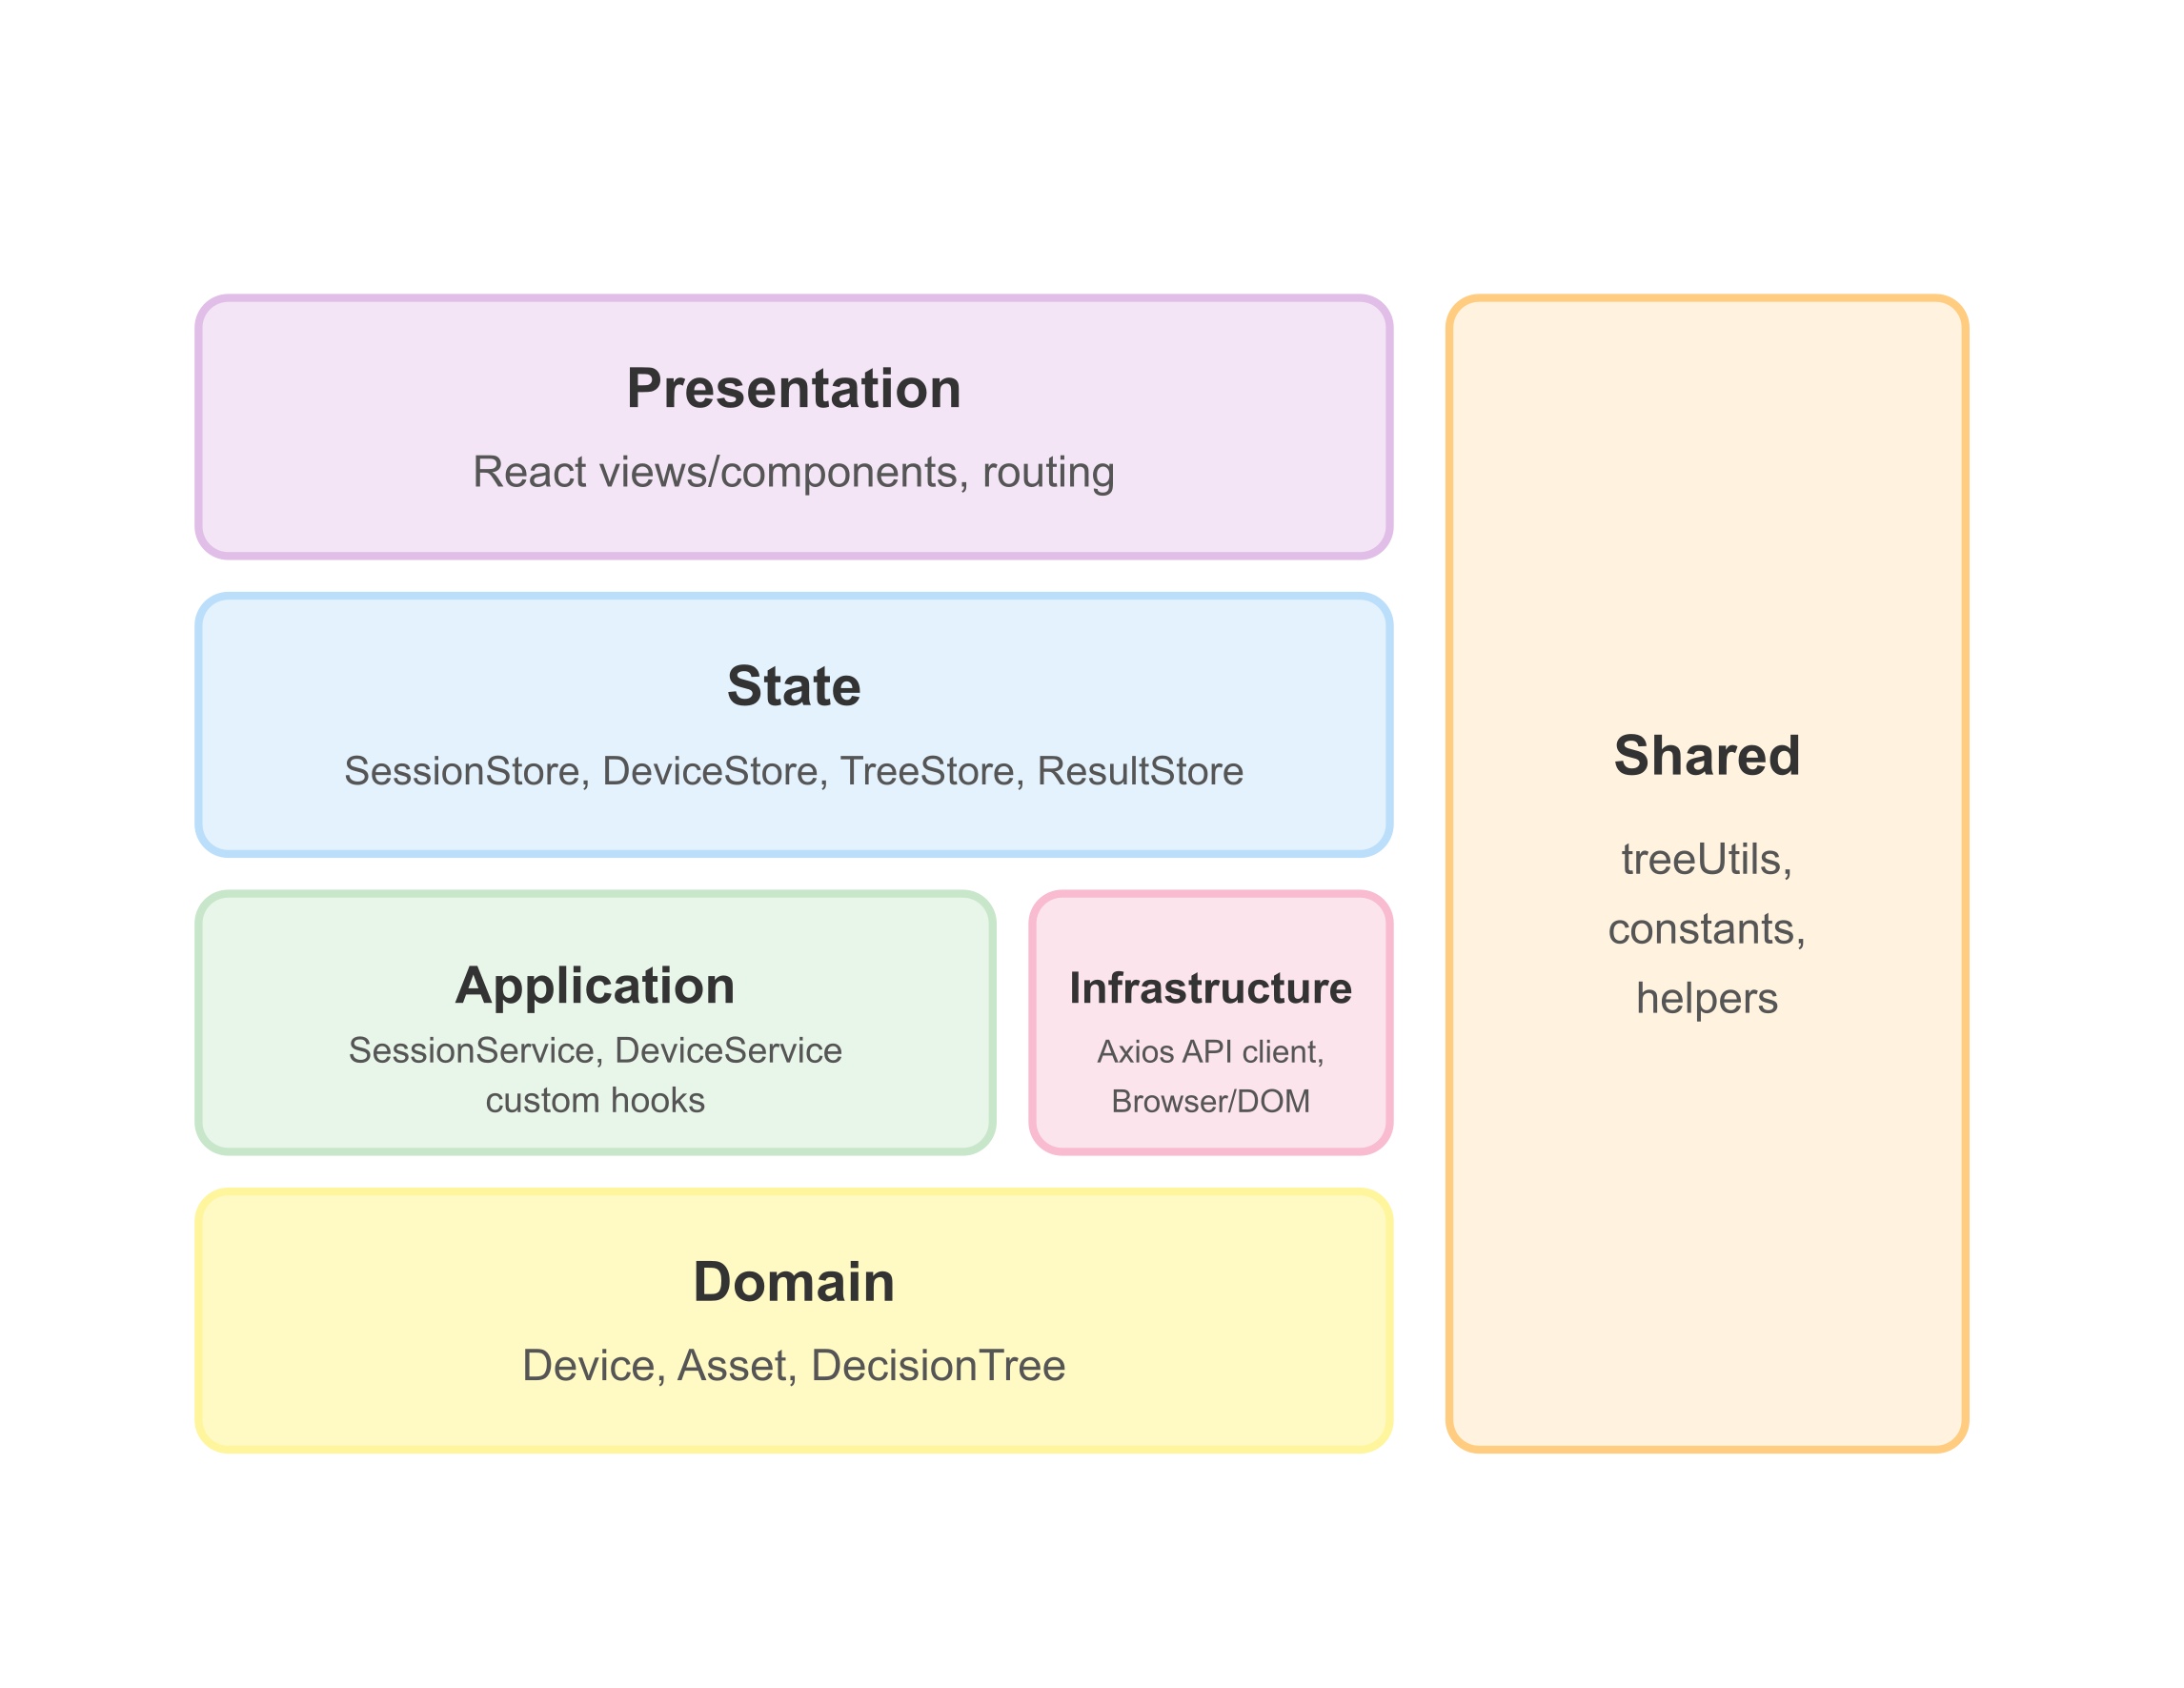
\includegraphics[width=.6\linewidth]{../../../Assets/classiFront/Layers.png}
                    \caption{Vista semplificata del frontend}
                \end{figure}
            \end{center}
            
            \paragraph{Layer di presentazione e routing}\mbox{}\\
            Il layer di presentazione comprende viste e componenti \textit{UI}\textsubscript{\href{https://atlasteam9.github.io/Atlas/glossario.html\#UI}{G}} riusabili. La navigazione è gestita tramite routing client-side e route guard che verificano le precondizioni dei flussi protetti (ad \textit{esempio}\textsubscript{\href{https://atlasteam9.github.io/Atlas/glossario.html\#Esempio}{G}} sessione attiva e dati dispositivo disponibili).  
            Questa organizzazione mantiene i componenti focalizzati sulla resa grafica e sull'esperienza utente, delegando l'orchestrazione ai livelli applicativi.
            
            \paragraph{Gestione dello stato}\mbox{}\\
            La gestione dello stato distingue tra:
            \begin{itemize}
                \item \textbf{stato globale}, condiviso tra più viste;
                \item \textbf{stato locale}, limitato al singolo componente o hook.
            \end{itemize}
            Lo stato globale è suddiviso in store separati per area funzionale (sessione, alberi decisionali, dispositivo, risultati, \textit{UI}\textsubscript{\href{https://atlasteam9.github.io/Atlas/glossario.html\#UI}{G}}), evitando uno stato monolitico.  
            L'uso di selector dedicati e compositi riduce duplicazioni di lettura e limita l'accoppiamento tra componenti.
            
            \paragraph{Layer applicativo: hook e servizi}\mbox{}\\
            La logica di orchestrazione è incapsulata in custom hook e \textit{servizi}\textsubscript{\href{https://atlasteam9.github.io/Atlas/glossario.html\#Servizi}{G}} applicativi.  
            I custom hook coordinano l'interazione tra vista, stato e \textit{servizi}\textsubscript{\href{https://atlasteam9.github.io/Atlas/glossario.html\#Servizi}{G}}; i \textit{servizi}\textsubscript{\href{https://atlasteam9.github.io/Atlas/glossario.html\#Servizi}{G}} applicativi centralizzano i casi d'uso principali (sessione, navigazione, export), mantenendo i componenti prevalentemente dichiarativi.  
            In coerenza con l'approccio pragmatico adottato, parte dell'orchestrazione applicativa interagisce direttamente con lo stato globale.
            
            \paragraph{Comunicazione con il backend}\mbox{}\\
            La comunicazione con il backend adotta principi ports-and-adapters in forma parziale:
            \begin{itemize}
                \item per l'accesso HTTP, il layer applicativo dipende da \textit{servizi}\textsubscript{\href{https://atlasteam9.github.io/Atlas/glossario.html\#Servizi}{G}} astratti;
                \item il layer infrastrutturale fornisce implementazioni concrete (client HTTP, adapter notifiche, mapping errori).
            \end{itemize}
            I payload ricevuti vengono convertiti in modelli frontend tramite mapper dedicati, così da disaccoppiare il dominio client dal formato esterno e contenere l'impatto di variazioni nei contratti API.
            
            \paragraph{Modello di dominio frontend}\mbox{}\\
            Il dominio frontend include entità principali (ad \textit{esempio}\textsubscript{\href{https://atlasteam9.github.io/Atlas/glossario.html\#Esempio}{G}} Device, Asset, Node, DecisionTree) e regole di business pure (filtri, valutazioni, trasformazioni).  
            L'incapsulamento dei dati e l'accesso controllato tramite metodi/getter migliorano consistenza del modello e robustezza delle regole applicative.

            
        \subsubsection{Design dettagliato frontend}
            Questa sezione approfondisce i moduli concreti del frontend, descrivendo ruolo e responsabilità di pagine, hook, store, \textit{servizi}\textsubscript{\href{https://atlasteam9.github.io/Atlas/glossario.html\#Servizi}{G}} e classi di dominio, nonché le loro interazioni nei principali flussi applicativi.

            \paragraph{Pages}\mbox{}\\
                Le pagine rappresentano il punto di ingresso dei principali casi d'uso utente e hanno la responsabilità di orchestrare la composizione dei componenti visuali e dei relativi hook applicativi.
                Ogni pagina mantiene un ruolo specifico nel flusso end-to-end, evitando sovrapposizioni funzionali.
                Descrizione sintetica delle principali pagine:
                \begin{itemize}
                    \item \texttt{HomeView}: schermata iniziale dell'applicazione, da essa è possibile avviare il flusso di creazione o caricamento del dispositivo da analizzare, o di caricamento di una sessione completa o incompleta.
                    \item \texttt{DeviceFormView}: schermata dedicata alla raccolta e \textit{validazione}\textsubscript{\href{https://atlasteam9.github.io/Atlas/glossario.html\#Validazione}{G}} dei dati descrittivi del dispositivo oggetto dell'analisi.
                    \item \texttt{DeviceAssetManagementView}: schermata per la gestione degli asset associati al dispositivo.
                    \item \texttt{AssetFormView}: schermata per la creazione del singolo asset.
                    \item \texttt{DeviceSummaryView}: presenta un riepilogo esaustivo dei dati inseriti prima dell'avvio del test.
                    \item \texttt{SessionRunnerView}: pagina che visualizza la domanda a cui l'utente deve rispondere e i componenti che permettono la gestione della navigazione tra le risposte.
                    \item \texttt{ResultView}: visualizza i risultati aggregati per \textit{requisito}\textsubscript{\href{https://atlasteam9.github.io/Atlas/glossario.html\#Requisito}{G}} e per asset, con opzioni di export.
                    \item \texttt{ModifySessionView}: pagina che permette la ripresa di una sessione incompleta o la modifica di una sessione completata tramite la selezione dell'asset da cui riprendere il percorso del test.
                \end{itemize}
                Linee guida adottate:
                \begin{itemize}
                    \item la pagina non contiene logica di business complessa;
                    \item la pagina delega la logica a hook e \textit{servizi}\textsubscript{\href{https://atlasteam9.github.io/Atlas/glossario.html\#Servizi}{G}};
                    \item la pagina mantiene responsabilità di composizione \textit{UI}\textsubscript{\href{https://atlasteam9.github.io/Atlas/glossario.html\#UI}{G}} e navigazione.
                \end{itemize}
                \begin{center}
                    \begin{figure}[H]
                        \centering
                        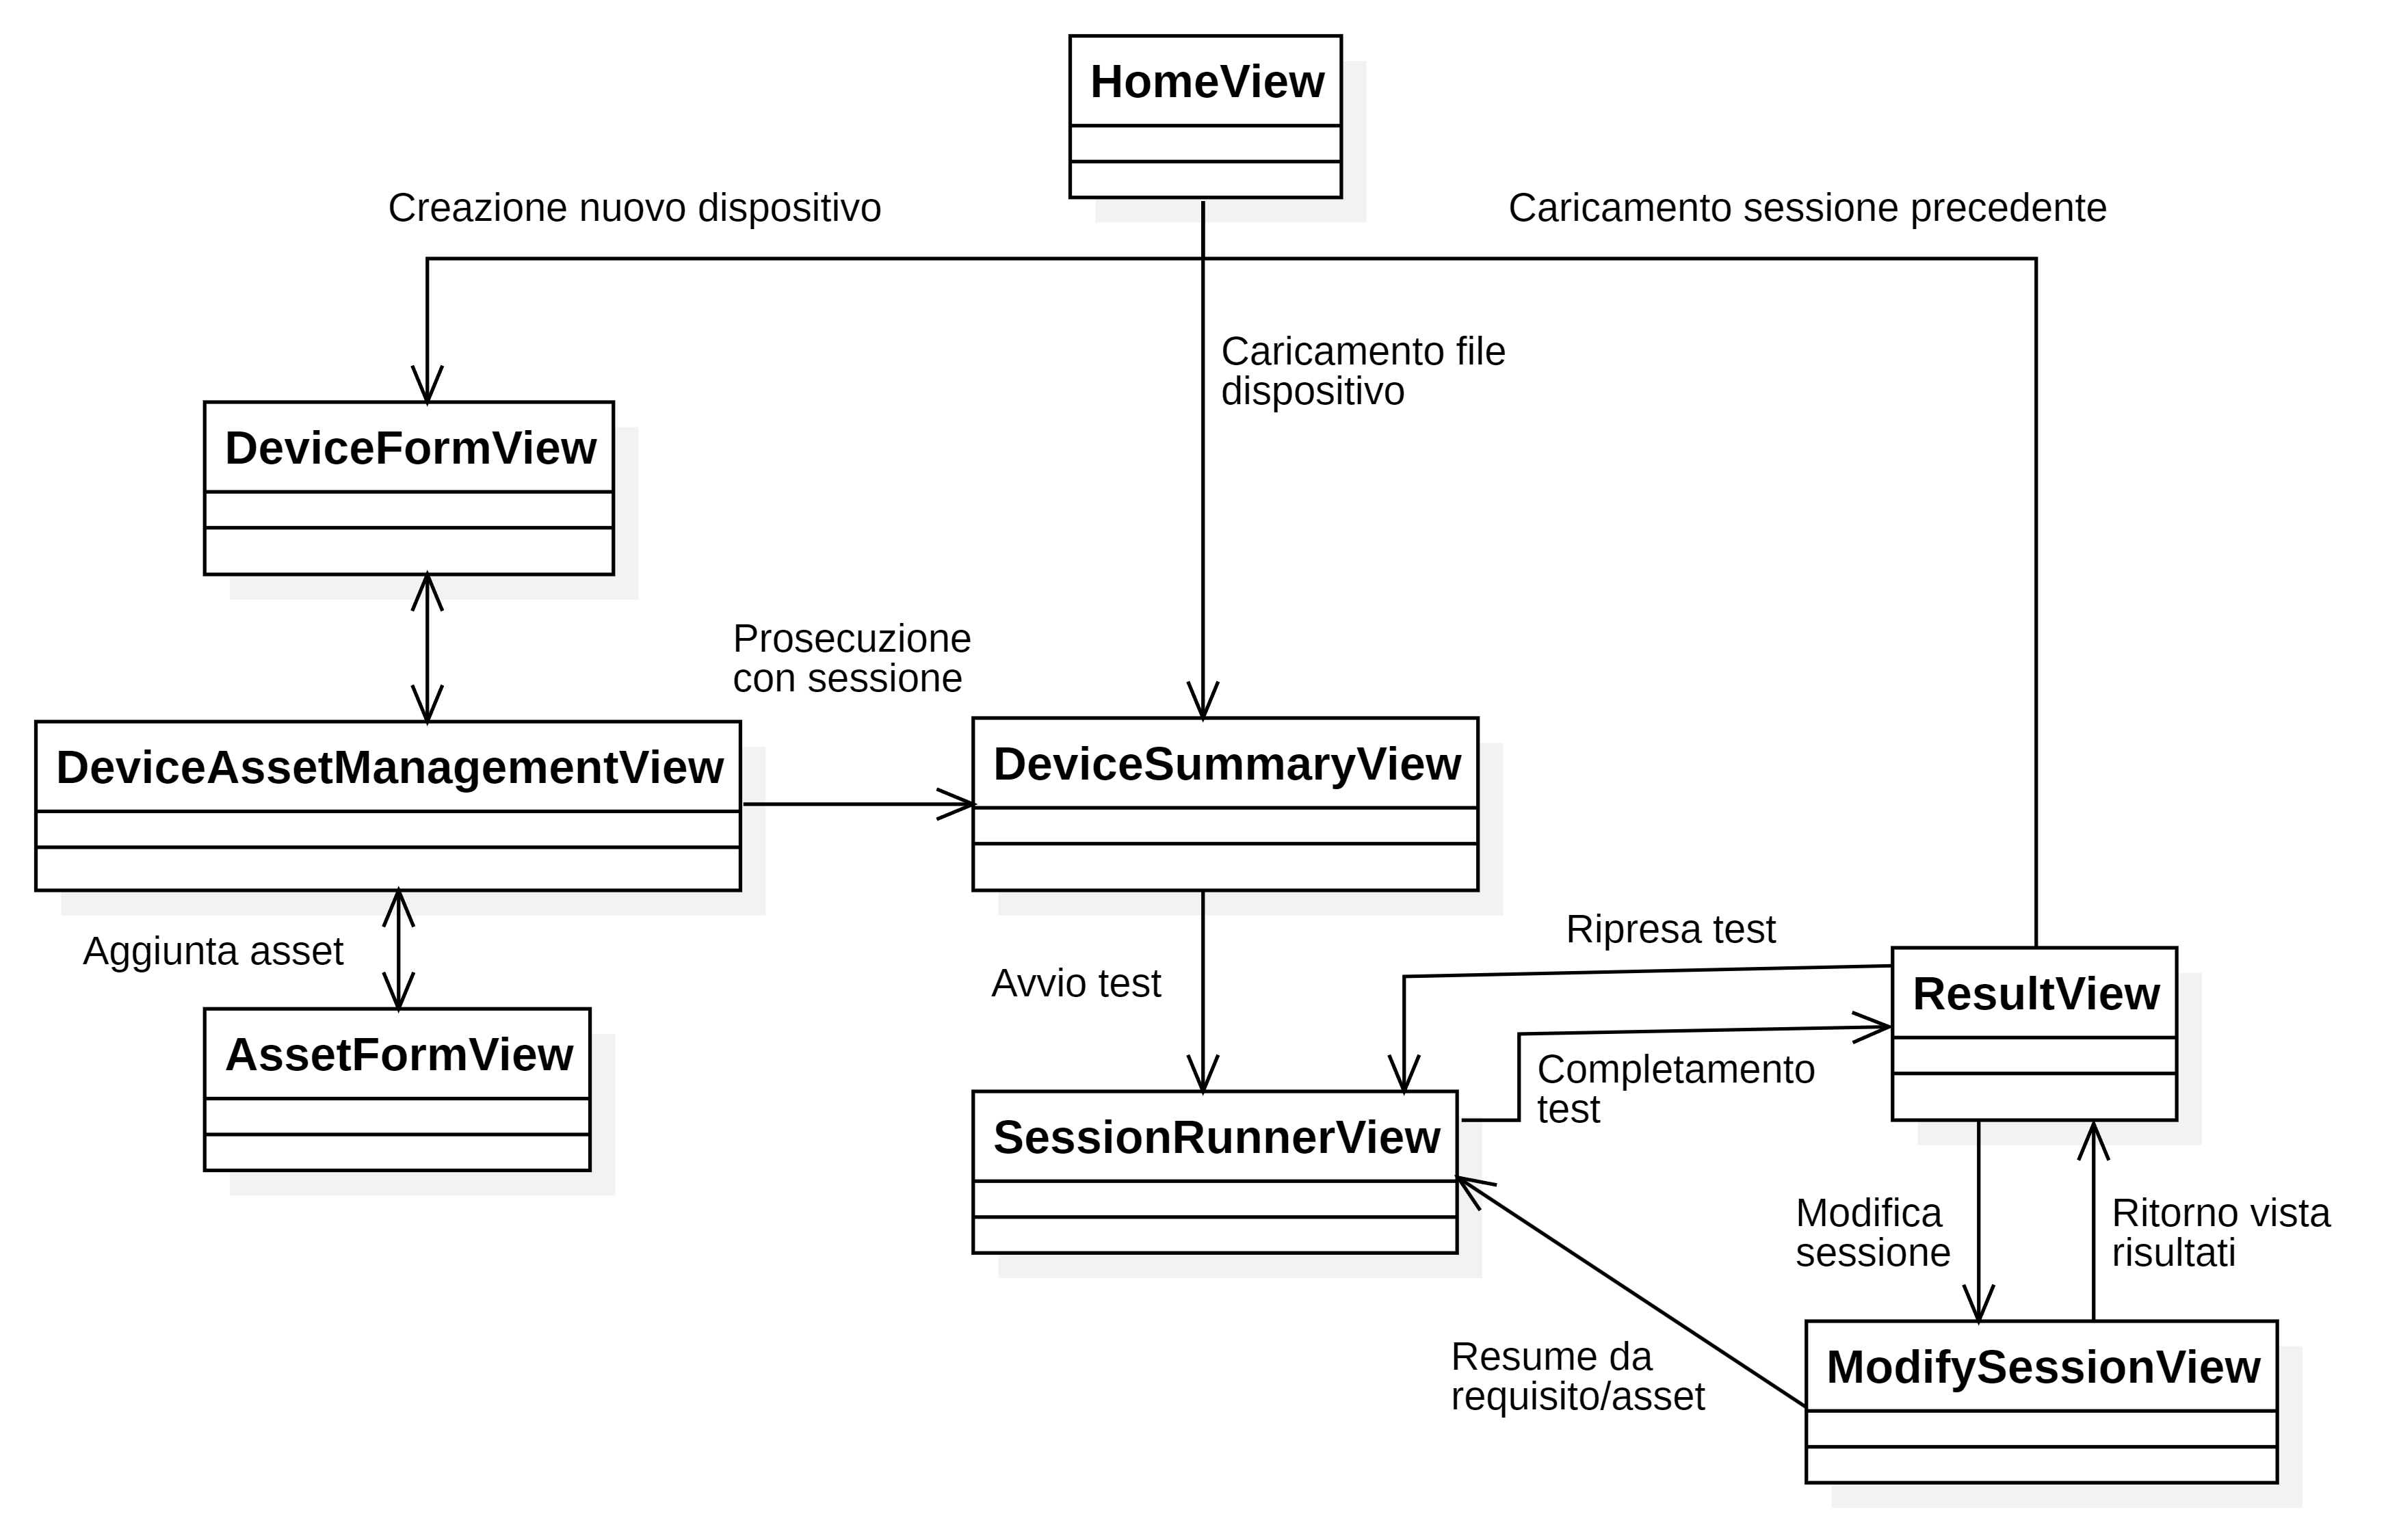
\includegraphics[width=.6\linewidth]{../../../Assets/classiFront/Pages.png}
                        \caption{Mappa pagine e transizioni}
                    \end{figure}
                \end{center}
        
            \paragraph{Componenti UI}\mbox{}\\
                I componenti \textit{UI}\textsubscript{\href{https://atlasteam9.github.io/Atlas/glossario.html\#UI}{G}} sono progettati per massimizzare riusabilità e separazione delle responsabilità: la presentazione resta nei componenti, mentre la logica applicativa viene delegata a hook, store e servizi. 
                Questo approccio riduce duplicazione, facilita il testing e rende più semplice l'evoluzione delle viste.
                
                Tipologie principali e componenti rappresentativi:
                \begin{itemize}
                    \item \textbf{Componenti trasversali}: \texttt{UploadButton}, \texttt{HomeIcon}, \texttt{BackIcon} e altri elementi riusabili impiegati in più viste.
                    \item \textbf{Input e form}: componenti usati nelle pagine \texttt{DeviceFormView} e \texttt{AssetFormView}, come \texttt{InputField}, \texttt{SelectField}, \texttt{CheckboxField} e \texttt{ToggleSwitch}.
                    \item \textbf{Resoconto dispositivo}: componenti usati nella pagina \texttt{DeviceSummaryView}, quali \newline \texttt{AssetInfoOverlay}, \texttt{AssetListView} che a sua volta contiene numerosi \texttt{AssetItemView}, \texttt{DeviceMainActions}, e altri sotto componenti.
                    \item \textbf{Supporto al flusso sessione}: \texttt{SessionContent}, \texttt{SessionContentAdapter} e sottocomponenti del runner per avanzamento, risposta e navigazione, come per \textit{esempio}\textsubscript{\href{https://atlasteam9.github.io/Atlas/glossario.html\#Esempio}{G}} \newline \texttt{AnswerButtons},  \texttt{NavigationFooter}, \texttt{QuestionSection} e \texttt{SessionHeader}.
                    \item \textbf{Visualizzazione risultati}: componenti utilizzati in \texttt{ResultView}, per \textit{esempio}\textsubscript{\href{https://atlasteam9.github.io/Atlas/glossario.html\#Esempio}{G}} \newline \texttt{ExportDialog}, \texttt{ResultListView}, \texttt{ResultItemView}, \texttt{AssetResultsView} e \texttt{ResultActions}.
                \end{itemize}
        
            \paragraph{Hook applicativi}\mbox{}\\
                I custom hook costituiscono il layer di orchestrazione tra \textit{UI}\textsubscript{\href{https://atlasteam9.github.io/Atlas/glossario.html\#UI}{G}}, stato globale e servizi. Essi incapsulano flussi operativi, side effect e coordinamento di navigazione, mantenendo i componenti dichiarativi. \\
                Hook principali:
                \begin{itemize}
                    \item \texttt{useHomeNavigation}: gestisce creazione/caricamento della sessione dalla home e la navigazione conseguente.
                    \item \texttt{useAssetManagement}: coordina la gestione degli asset, del salvataggio dispositivo, dei controlli sulle modifiche non salvate e il passaggio alla vista di resoconto.
                    \item \texttt{useResultViewLogic}: centralizza la logica della vista risultati, come l'espansione requisiti, la ripresa, l'export e il ritorno alla home.
                    \item \texttt{useModifySessionLogic}: gestisce la selezione del requisito/asset e la ripresa del test.
                    \item \texttt{useRouteGuardAccess}: verifica le precondizioni di accesso alle pagine protette.
                    \item \texttt{useTreeBootstrap}: effettua il bootstrap iniziale dei decision tree.
                    \item \texttt{useSessionRunnerTrees}: espone i tree necessari al runner.
                    \item \texttt{useBeforeUnload}: gestisce la protezione in uscita durante operazioni sensibili.
                    \item \texttt{useExportResults} / \texttt{useExportSession}: gestiscono i flussi di \textit{esportazione}\textsubscript{\href{https://atlasteam9.github.io/Atlas/glossario.html\#Esportazione}{G}} e i relativi stati.
                \end{itemize}
                Hook specifici del flusso sessione:
                \begin{itemize}
                    \item \texttt{useSessionState}: aggrega lo stato della sessione utile alla vista runner.
                    \item \texttt{useSessionHandlers}: espone handler asincroni (invio risposta, navigazione, salvataggio/uscita) con gestione uniforme di loading/error.
                    \item \texttt{useSessionRedirect}: gestisce redirect coerenti in caso di stato sessione non valido.
                \end{itemize}
        
            \paragraph{State management (store e selectors)}\mbox{}\\
                La gestione dello stato globale è strutturata in store separati per contesto funzionale. Ogni store definisce il proprio stato, le azioni di modifica e le relative invarianti. L'accesso agli store avviene tramite selectors, che permettono di astrarre la forma interna dello stato e ridurre l'accoppiamento tra consumer e struttura store. \\
                Gli store principali sono:
                \begin{itemize}
                    \item \texttt{SessionStore}: mantiene lo stato di sessione, ovvero id, posizione corrente, storia delle risposte, la modalità ripresa, i risultati per asset, lo stato fine test, e le azioni di navigazione nel flusso.
                    \item \texttt{TreeStore}: mantiene i \textit{decision tree}\textsubscript{\href{https://atlasteam9.github.io/Atlas/glossario.html\#DecisionTree}{G}} normalizzati e fornisce l'accesso ai nodi.
                    \item \texttt{DeviceStore}: mantiene il dispositivo corrente e la gestione degli asset ad esso associati.
                    \item \texttt{ResultStore}: mantiene i risultati aggregati del test.
                    \item \texttt{UIStore}: mantiene stati trasversali di \textit{interfaccia}\textsubscript{\href{https://atlasteam9.github.io/Atlas/glossario.html\#Interfaccia}{G}} (loading, exporting, dirty flag).
                \end{itemize}
        
            \paragraph{Services (application e infrastructure)}\mbox{}\\
                I \textit{servizi}\textsubscript{\href{https://atlasteam9.github.io/Atlas/glossario.html\#Servizi}{G}} implementano operazioni applicative e integrazioni tecniche. La distinzione principale è tra:
                \begin{itemize}
                    \item \textit{servizi}\textsubscript{\href{https://atlasteam9.github.io/Atlas/glossario.html\#Servizi}{G}} applicativi, orientati ai casi d'uso;
                    \item \textit{servizi}\textsubscript{\href{https://atlasteam9.github.io/Atlas/glossario.html\#Servizi}{G}} infrastrutturali, orientati a dettagli tecnici.
                \end{itemize}
                \textit{Servizi}\textsubscript{\href{https://atlasteam9.github.io/Atlas/glossario.html\#Servizi}{G}} applicativi:
                \begin{itemize}
                    \item \texttt{SessionService}: è il servizio principale del flusso sessione (creazione, caricamento, invio risposta, navigazione avanti/indietro, ripresa, pulizia, salvataggio e uscita).
                    \item \texttt{TreeService}: per il caricamento e la normalizzazione dei decision tree.
                    \item \texttt{DeviceService}: per la gestione del dispositivo corrente e le operazioni sugli asset.
                    \item \texttt{ExportService}: per l'\textit{esportazione}\textsubscript{\href{https://atlasteam9.github.io/Atlas/glossario.html\#Esportazione}{G}} di risultati/sessione/dispositivo.
                    \item \texttt{NavigationService}: servizio di utilità per il reset dello stato e la navigazione verso la pagina home.
                    \item \texttt{ApiClientService}: wrapper applicativo della porta API.
                    \item \texttt{NotificationService}: wrapper applicativo della porta notifiche.
                \end{itemize}
                Servizi/adapter infrastrutturali:
                \begin{itemize}
                    \item \texttt{AxiosApiClient}: implementazione concreta del client HTTP.
                    \item \texttt{errorMapper}: conversione errori tecnici in errori applicativi.
                    \item \texttt{NotificationManager} + \texttt{SonnerNotificationAdapter}: gestione notifiche utente.
                \end{itemize}
        
            \paragraph{Domain e regole di business}\mbox{}\\
                Il dominio frontend contiene entità e regole pure che modellano il problema applicativo anche lato client. Le classi dominio adottano incapsulamento dei dati e \textit{API}\textsubscript{\href{https://atlasteam9.github.io/Atlas/glossario.html\#API}{G}} esplicite, mentre le regole pure sono mantenute in funzioni dedicate. \\
                Responsabilità del dominio:
                \begin{itemize}
                    \item rappresentare in modo consistente dispositivi, asset, nodi e alberi;
                    \item fornire trasformazioni controllate da/verso payload esterni;
                    \item centralizzare regole di filtro/valutazione indipendenti dalla UI.
                \end{itemize}
                Classi principali:
                \begin{itemize}
                    \item \texttt{Device}: modello del dispositivo con metodi di gestione asset e serializzazione.
                    \item \texttt{Asset}: modello del singolo asset con tipo, sensibilità e serializzazione.
                    \item \texttt{Node}: modello del \textit{nodo}\textsubscript{\href{https://atlasteam9.github.io/Atlas/glossario.html\#Nodo}{G}} decisionale (domanda/risultato).
                    \item \texttt{DecisionTree}: modello del \textit{requisito}\textsubscript{\href{https://atlasteam9.github.io/Atlas/glossario.html\#Requisito}{G}} con nodi e dipendenze, che trasforma le informazioni grezze del backend in oggetti pronti per l'applicazione.
                \end{itemize}
                
                Regole e \textit{validazione}\textsubscript{\href{https://atlasteam9.github.io/Atlas/glossario.html\#Validazione}{G}}:
                \begin{itemize}
                    \item \texttt{treeRules}: regole pure per filtraggio/valutazione risultati riprendibili.
                    \item \texttt{AssetSchema}, \texttt{DeviceSchema}: \textit{validazione}\textsubscript{\href{https://atlasteam9.github.io/Atlas/glossario.html\#Validazione}{G}} strutturale dei dati di \textit{input}\textsubscript{\href{https://atlasteam9.github.io/Atlas/glossario.html\#Input}{G}} di asset e device.
                \end{itemize}
        
        \subsubsection{Caratteristiche di qualità}
            \paragraph{Manutenibilità}\mbox{}\\
                La separazione per layer, l'uso di selector e la centralizzazione dei \textit{servizi}\textsubscript{\href{https://atlasteam9.github.io/Atlas/glossario.html\#Servizi}{G}} migliorano la manutenibilità in presenza di evoluzioni funzionali o tecniche.
                
            \paragraph{Scalabilità}\mbox{}\\
                La struttura attuale supporta estensioni progressive:
                \begin{itemize}
                    \item nuove pagine senza impatto sul dominio;
                    \item nuovi flussi applicativi tramite hook/servizi dedicati;
                    \item sostituzione di adapter infrastrutturali con impatto contenuto.
                \end{itemize}

        \subsubsection{Elementi principali}
            \paragraph{Classi del dominio}
                \subparagraph{Asset}
                    \begin{center}
                        \begin{figure}[H]
                            \centering
                            
\includegraphics[width=.6\linewidth]{../../../Assets/classiFront/Asset.png}
                            \caption{Asset: classe frontend}
                        \end{figure}
                    \end{center}
                    Rappresenta un singolo componente da testare.\\\\
                    \textbf{Attributi}
                    \begin{itemize}
                        \item {\ttfamily id}: id univoco dell'asset;
                        \item {\ttfamily name}: nome dell'asset;
                        \item {\ttfamily type}: tipo dell'asset;
                        \item {\ttfamily isSensitive}: flag di sensibilità dell'asset;
                        \item {\ttfamily desc}: descrizione (opzionale) dell'asset.
                    \end{itemize}
                    \textbf{Metodi}
                        \begin{itemize}
                            \item Metodi getter per ogni attributo;
                            \item {\ttfamily toDict(): Dictionary}: metodo utilizzato per la serializzazione.
                        \end{itemize}
                    
            \subparagraph{Device}\mbox{}\\

                \begin{center}
                    \begin{figure}[H]
                        \centering
                        
\includegraphics[width=.3\linewidth]{../../../Assets/classiFront/Device.png}
                        \caption{Device: classe frontend}
                    \end{figure}
                \end{center}
                Rappresenta il dispositivo facente uso di onde radio oggetto della valutazione. Aggrega una \textit{lista}\textsubscript{\href{https://atlasteam9.github.io/Atlas/glossario.html\#Lista}{G}} di Asset e contiene le informazioni generali del dispositivo.\\\\
                \textbf{Attributi}
                \begin{itemize}
                    \item {\ttfamily name}: nome del dispositivo;
                    \item {\ttfamily assets[]}: \textit{lista}\textsubscript{\href{https://atlasteam9.github.io/Atlas/glossario.html\#Lista}{G}} di oggetti Asset;
                    \item {\ttfamily operatingSystem}: sistema operativo del dispositivo;
                    \item {\ttfamily firmwareVersion}: versione del \textit{firmware}\textsubscript{\href{https://atlasteam9.github.io/Atlas/glossario.html\#Firmware}{G}} del dispositivo;
                    \item {\ttfamily functionalities}: funzionalità del dispositivo;
                    \item {\ttfamily description}: descrizione del dispositivo (opzionale).
                \end{itemize}
                \textbf{Metodi}
                    \begin{itemize}
                        \item Metodi getter per ogni attributo;
                        \item {\ttfamily addAsset(asset)}: aggiunge un asset in coda all'array degli asset;
                        \item {\ttfamily deleteAsset(assetId)}: elimina dall'array l'asset con l'identificativo passato per parametro;
                        \item {\ttfamily toDict(): Dictionary}: metodo utilizzato per la serializzazione.
                    \end{itemize}
            
            \subparagraph{Node}\mbox{}\\

                \begin{center}
                    \begin{figure}[H]
                        \centering
                        
\includegraphics[width=.6\linewidth]{../../../Assets/classiFront/Node.png}
                        \caption{Node: classe frontend}
                    \end{figure}
                \end{center}
                Rappresenta un \textit{nodo}\textsubscript{\href{https://atlasteam9.github.io/Atlas/glossario.html\#Nodo}{G}} di un decision tree.\\\\
                \textbf{Attributi}
                \begin{itemize}
                    \item {\ttfamily id}: id del \textit{nodo}\textsubscript{\href{https://atlasteam9.github.io/Atlas/glossario.html\#Nodo}{G}};
                    \item {\ttfamily text}: contenuto principale del \textit{nodo}\textsubscript{\href{https://atlasteam9.github.io/Atlas/glossario.html\#Nodo}{G}}, che può essere una domanda o il testo del risultato;
                    \item {\ttfamily description}: descrizione del \textit{nodo}\textsubscript{\href{https://atlasteam9.github.io/Atlas/glossario.html\#Nodo}{G}} (opzionale);
                    \item {\ttfamily type}: indica la natura del \textit{nodo}\textsubscript{\href{https://atlasteam9.github.io/Atlas/glossario.html\#Nodo}{G}}, può essere "QUESTION" oppure "RESULT".
                \end{itemize}
                \textbf{Metodi}
                    \begin{itemize}
                        \item Metodi getter per ogni attributo.
                        \item {\ttfamily fromApi(nodeId, nodeData): Node}: utilizzato per trasformare il formato grezzo che arriva dal backend in un oggetto Node.
                    \end{itemize}

            \subparagraph{DecisionTree}\mbox{}\\

                \begin{center}
                    \begin{figure}[H]
                        \centering
                        
\includegraphics[width=.3\linewidth]{../../../Assets/classiFront/DecisionTree.png}
                        \caption{DecisionTree: classe frontend}
                    \end{figure}
                \end{center}
                Albero decisionale corrispondente ad un \textit{requisito}\textsubscript{\href{https://atlasteam9.github.io/Atlas/glossario.html\#Requisito}{G}} della \textit{norma}\textsubscript{\href{https://atlasteam9.github.io/Atlas/glossario.html\#Norma}{G}} EN 18031.\\\\
                \textbf{Attributi}
                \begin{itemize}
                    \item {\ttfamily id: String}: id dell'albero;
                    \item {\ttfamily title}: titolo dell'albero (nome del \textit{requisito}\textsubscript{\href{https://atlasteam9.github.io/Atlas/glossario.html\#Requisito}{G}});
                    \item {\ttfamily nodes\{\}}: mappa dei nodi del \textit{decision tree}\textsubscript{\href{https://atlasteam9.github.io/Atlas/glossario.html\#DecisionTree}{G}};
                    \item {\ttfamily dependencies[]}: \textit{lista}\textsubscript{\href{https://atlasteam9.github.io/Atlas/glossario.html\#Lista}{G}} delle dipendenze dell'albero.
                \end{itemize}
                \textbf{Metodi}
                    \begin{itemize}
                        \item Metodi getter per ogni attributo.
                        \item {\ttfamily getNodeById(nodeId)}: metodo per ritornare un \textit{nodo}\textsubscript{\href{https://atlasteam9.github.io/Atlas/glossario.html\#Nodo}{G}} dell'albero da un identificativo passato per parametro;
                        \item {\ttfamily fromApi(treeData): DecisionTree}: utilizzato per trasformare il formato grezzo che arriva dal backend in un oggetto DecisionTree.
                    \end{itemize}

        % DESCRIZIONE \textit{SERVIZI}\textsubscript{\href{https://atlasteam9.github.io/Atlas/glossario.html\#Servizi}{G}} FRONTEND 
            \paragraph{Servizi applicativi}
                \subparagraph{ApiClientService}
                \begin{center}
                    \begin{figure}[H]
                        \centering
                        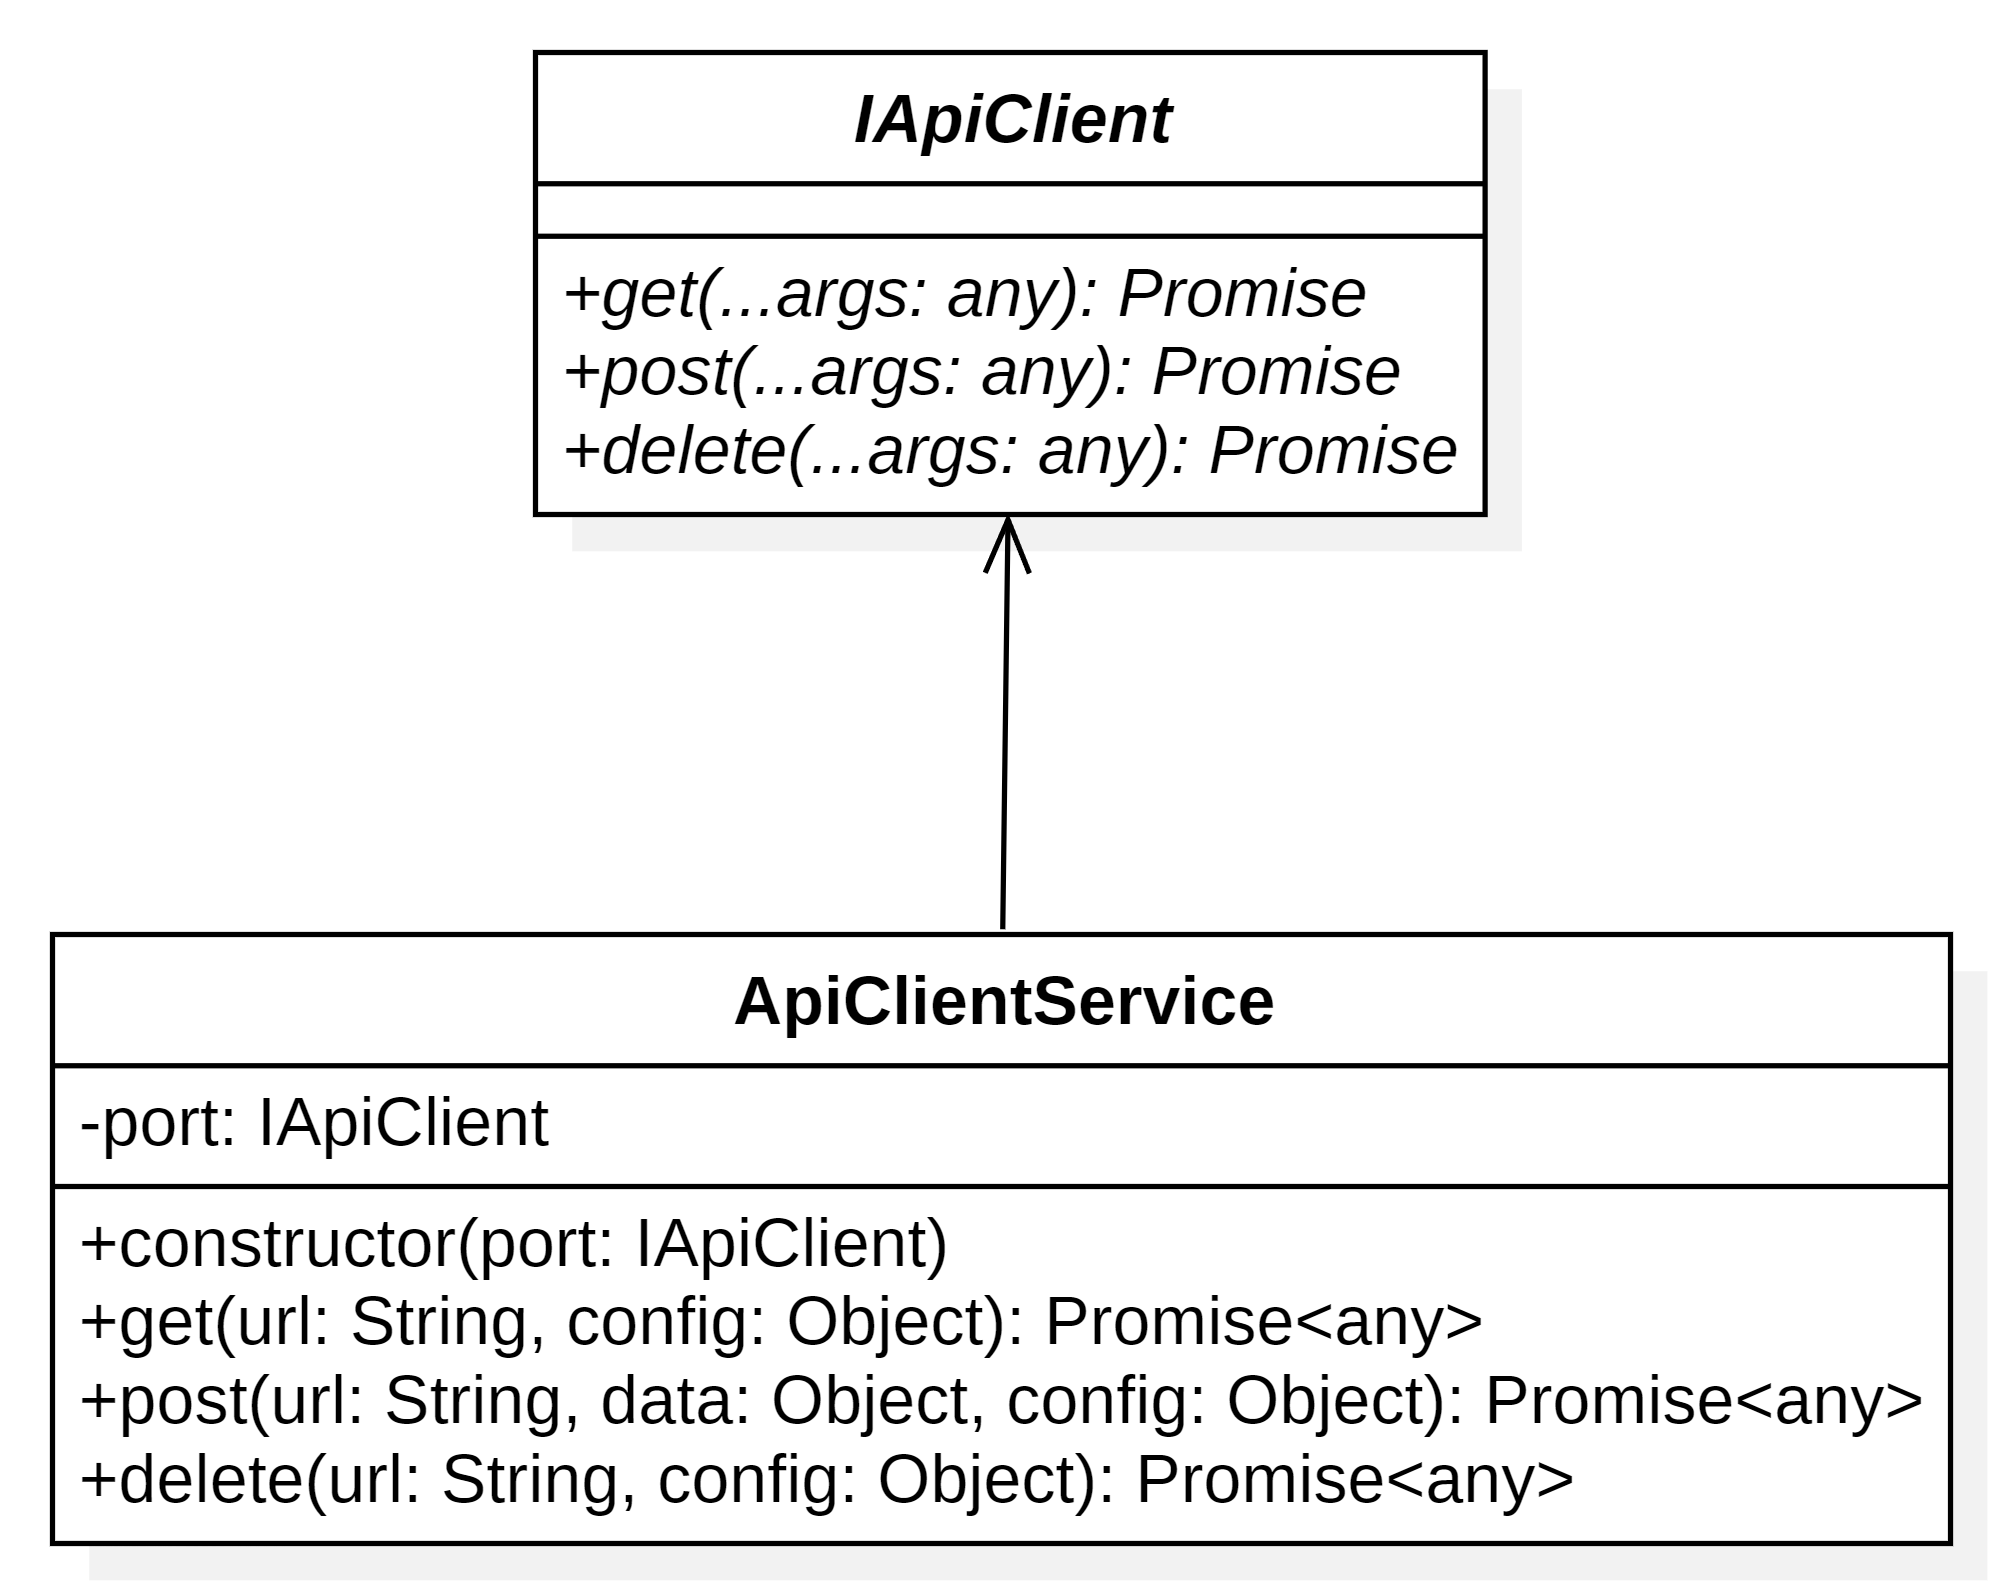
\includegraphics[width=.4\linewidth]{../../../Assets/classiFront/ApiClientService.png}
                        \caption{ApiClientService: classe application}
                    \end{figure}
                \end{center}
                Servizio applicativo che incapsula il client HTTP tramite porta astratta (\texttt{IApiClient}), così il layer application non dipende direttamente da Axios o da altri adapter concreti.\\\\
                \textbf{Attributi}
                \begin{itemize}
                    \item {\ttfamily port}: riferimento alla porta HTTP che deve implementare {\ttfamily get}, {\ttfamily post}, {\ttfamily delete}.
                \end{itemize}
                \textbf{Metodi}
                \begin{itemize}
                    \item {\ttfamily constructor(port)}: valida che la porta implementi i metodi richiesti;
                    \item {\ttfamily get(url, config)}: inoltra una GET alla porta;
                    \item {\ttfamily post(url, data, config)}: inoltra una POST alla porta;
                    \item {\ttfamily delete(url, config)}: inoltra una DELETE alla porta.
                \end{itemize}
                
                \subparagraph{NotificationService}\mbox{}\
                
                \begin{center}
                    \begin{figure}[H]
                        \centering
                        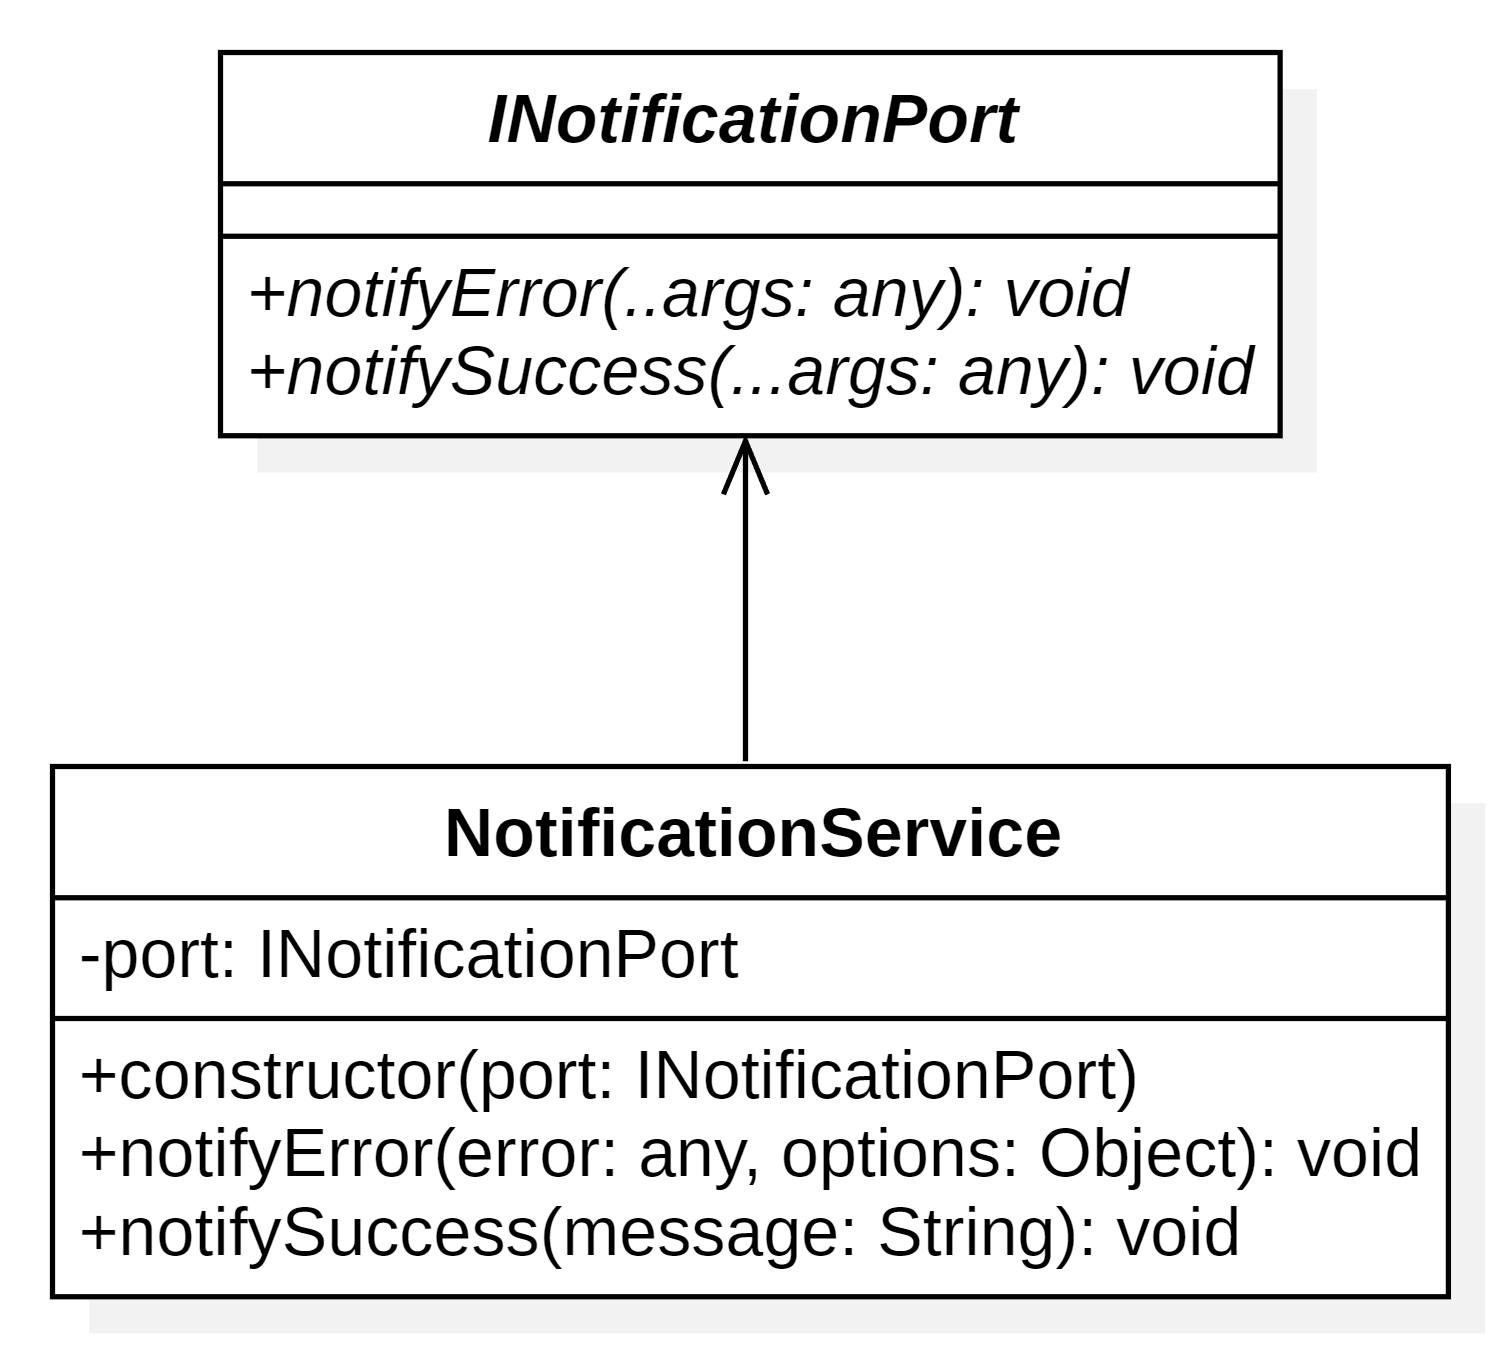
\includegraphics[width=.4\linewidth]{../../../Assets/classiFront/NotificationService.png}
                        \caption{NotificationService: classe application}
                    \end{figure}
                \end{center}
                Servizio applicativo per notifiche utente, disaccoppiato dal \textit{framework}\textsubscript{\href{https://atlasteam9.github.io/Atlas/glossario.html\#Framework}{G}} \textit{UI}\textsubscript{\href{https://atlasteam9.github.io/Atlas/glossario.html\#UI}{G}} tramite porta \newline {\ttfamily INotificationPort}.\\\\
                \textbf{Attributi}
                \begin{itemize}
                    \item {\ttfamily port}: riferimento all'adapter di notifica concreto (es. Sonner), che espone metodi di notifica.
                \end{itemize}
                \textbf{Metodi}
                \begin{itemize}
                    \item {\ttfamily constructor(port)}: valida che la porta implementi {\ttfamily notifyError} e {\ttfamily notifySuccess};
                    \item {\ttfamily notifyError(error, options)}: mostra una notifica di \textit{errore}\textsubscript{\href{https://atlasteam9.github.io/Atlas/glossario.html\#Errore}{G}};
                    \item {\ttfamily notifySuccess(message)}: mostra una notifica di successo.
                \end{itemize}
                
                \subparagraph{DeviceService}\mbox{}\
                
                \begin{center}
                    \begin{figure}[H]
                        \centering
                        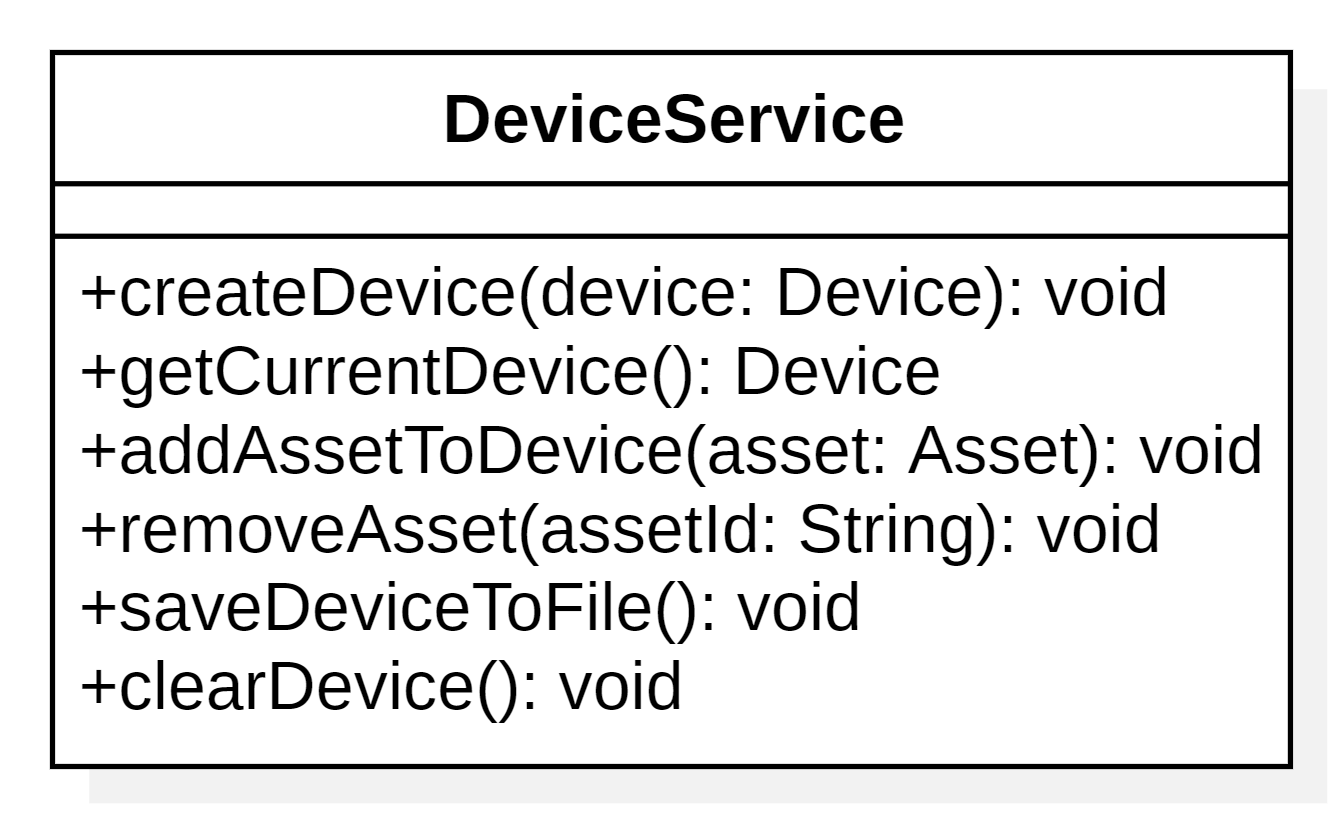
\includegraphics[width=.4\linewidth]{../../../Assets/classiFront/DeviceService.png}
                        \caption{DeviceService: classe application}
                    \end{figure}
                \end{center}
                Servizio applicativo per la gestione del dispositivo corrente e dei suoi asset, orchestrando i relativi store di stato.\\
                \textbf{Attributi}
                \begin{itemize}
                    \item Nessun attributo di istanza persistente (servizio stateless, usa gli store globali).
                \end{itemize}
                \textbf{Metodi}
                \begin{itemize}
                    \item {\ttfamily createDevice(device)}: salva il dispositivo nello stato applicativo;
                    \item {\ttfamily getCurrentDevice()}: restituisce il dispositivo corrente;
                    \item {\ttfamily addAssetToDevice(asset)}: aggiunge un asset al dispositivo e marca lo stato come modificato;
                    \item {\ttfamily removeAsset(assetId)}: rimuove un asset dal dispositivo e marca lo stato come modificato;
                    \item {\ttfamily saveDeviceToFile()}: esporta il device in JSON e resetta il flag di modifiche;
                    \item {\ttfamily clearDevice()}: pulisce il device dallo stato locale.
                \end{itemize}
                
                \subparagraph{TreeService}\mbox{}\
                
                \begin{center}
                    \begin{figure}[H]
                        \centering
                        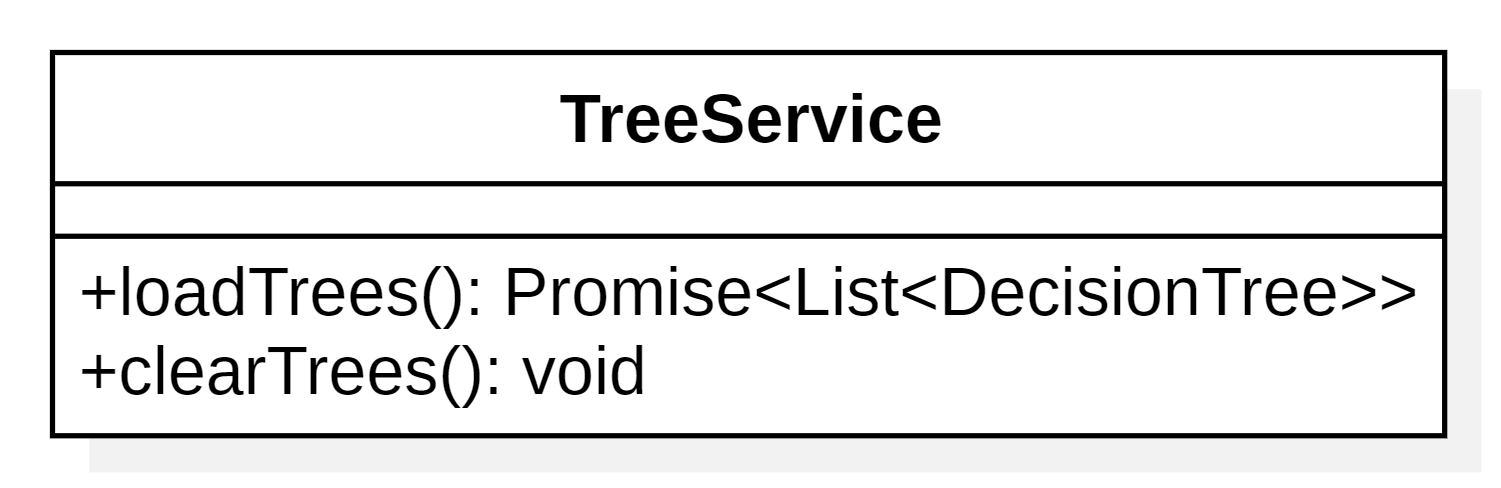
\includegraphics[width=.4\linewidth]{../../../Assets/classiFront/TreeService.png}
                        \caption{TreeService: classe application}
                    \end{figure}
                \end{center}
                Servizio applicativo per il caricamento dei \textit{decision tree}\textsubscript{\href{https://atlasteam9.github.io/Atlas/glossario.html\#DecisionTree}{G}} dal backend e la sincronizzazione nello store frontend.\\\\
                \textbf{Attributi}
                \begin{itemize}
                    \item Nessun attributo di istanza persistente (usa servizi/store condivisi).
                \end{itemize}
                \textbf{Metodi}
                \begin{itemize}
                    \item {\ttfamily loadTrees()}: recupera i tree da \textit{API}\textsubscript{\href{https://atlasteam9.github.io/Atlas/glossario.html\#API}{G}}, li normalizza in oggetti {\ttfamily DecisionTree} e salva gli alberi normalizzati nello stato applicativo;
                    \item {\ttfamily clearTrees()}: svuota i tree dallo store.
                \end{itemize}
                
                \subparagraph{SessionService}\mbox{}\
                
                \begin{center}
                    \begin{figure}[H]
                        \centering
                        
\includegraphics[width=.5\linewidth]{../../../Assets/classiFront/SessionService.png}
                        \caption{SessionService: classe application}
                    \end{figure}
                \end{center}
                Servizio applicativo centrale per l'orchestrazione dell'intero flusso di sessione: creazione, invio risposte, navigazione, caricamento/salvataggio e ripresa test.\\\\
                \textbf{Attributi}
                \begin{itemize}
                    \item Nessun attributo pubblico persistente; usa store e helper del layer application.
                \end{itemize}
                \textbf{Metodi}
                \begin{itemize}
                    \item {\ttfamily initializeSessionFromResponse(response)}: metodo privato per inizializzare stato locale da risposta backend;
                    \item {\ttfamily createSessionWithFile(file)}: crea sessione da file JSON caricato;
                    \item {\ttfamily createSessionWithDevice(device)}: crea sessione da oggetto Device serializzato;
                    \item {\ttfamily sendAnswer(answer)}: invia risposta e gestisce avanzamento/go-back/fine albero;
                    \item {\ttfamily previousStep()}: naviga localmente al \textit{nodo}\textsubscript{\href{https://atlasteam9.github.io/Atlas/glossario.html\#Nodo}{G}} precedente;
                    \item {\ttfamily forwardStep()}: naviga localmente al \textit{nodo}\textsubscript{\href{https://atlasteam9.github.io/Atlas/glossario.html\#Nodo}{G}} successivo;
                    \item {\ttfamily loadSessionFromFile(file)}: ripristina una sessione esportata in file JSON;
                    \item {\ttfamily saveAndExit()}: chiude sessione remota e pulisce stato locale;
                    \item {\ttfamily getSessionId()}: restituisce l'identificativo sessione corrente;
                    \item {\ttfamily getFormattedAnswers()}: converte lo storico risposte nel payload \textit{API}\textsubscript{\href{https://atlasteam9.github.io/Atlas/glossario.html\#API}{G}};
                    \item {\ttfamily clearSession()}: cancella la sessione corrente (remota e locale);
                    \item {\ttfamily resumeSession(requirementId, assetId)}: riposiziona la sessione su requisito/asset scelto.
                \end{itemize}
                
                \subparagraph{ExportService}\mbox{}\
                \begin{center}
                    \begin{figure}[H]
                        \centering
                        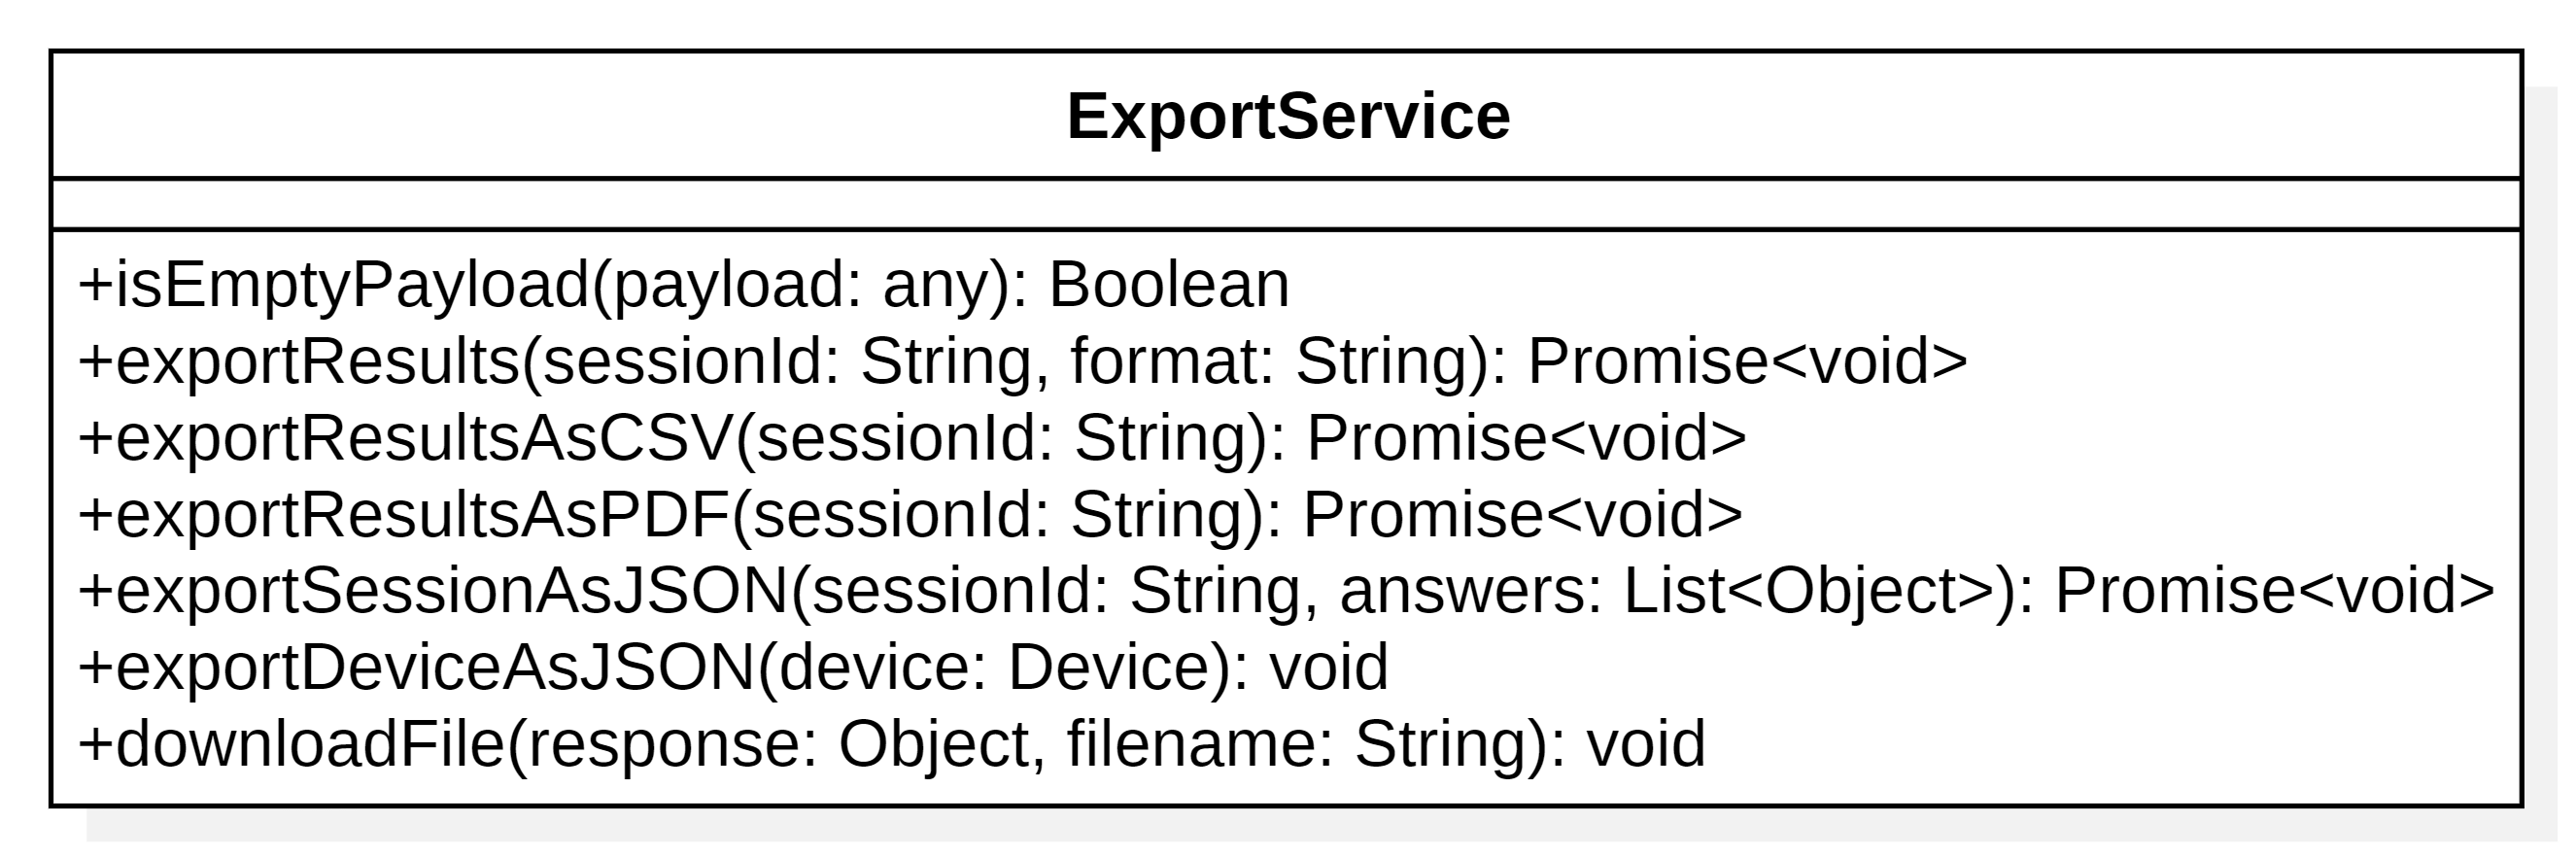
\includegraphics[width=.5\linewidth]{../../../Assets/classiFront/ExportService.png}
                        \caption{ExportService: classe application}
                    \end{figure}
                \end{center}
                Servizio applicativo per \textit{esportazione}\textsubscript{\href{https://atlasteam9.github.io/Atlas/glossario.html\#Esportazione}{G}} risultati/sessione/device in diversi formati, con \textit{validazione}\textsubscript{\href{https://atlasteam9.github.io/Atlas/glossario.html\#Validazione}{G}} payload e download file.\\\\
                \textbf{Attributi}
                \begin{itemize}
                    \item Nessun attributo di istanza persistente.
                \end{itemize}
                \textbf{Metodi}
                \begin{itemize}
                    \item {\ttfamily isEmptyPayload(payload)}: verifica se il payload ricevuto è vuoto/non valido;
                    \item {\ttfamily exportResults(sessionId, format)}: esporta i risultati della sessione in formato richiesto;
                    \item {\ttfamily exportResultsAsCSV(sessionId)}: shortcut per \textit{esportazione}\textsubscript{\href{https://atlasteam9.github.io/Atlas/glossario.html\#Esportazione}{G}} \textit{CSV}\textsubscript{\href{https://atlasteam9.github.io/Atlas/glossario.html\#CSV}{G}};
                    \item {\ttfamily exportResultsAsPDF(sessionId)}: shortcut per \textit{esportazione}\textsubscript{\href{https://atlasteam9.github.io/Atlas/glossario.html\#Esportazione}{G}} \textit{PDF}\textsubscript{\href{https://atlasteam9.github.io/Atlas/glossario.html\#PDF}{G}};
                    \item {\ttfamily exportSessionAsJSON(sessionId, answers)}: esporta la sessione completa come JSON;
                    \item {\ttfamily exportDeviceAsJSON(device)}: esporta il device corrente in JSON;
                    \item {\ttfamily downloadFile(response, filename)}: helper per avviare il download nel browser.
                \end{itemize}
                
                \subparagraph{AppError (e sottoclassi)}\mbox{}\
                
                \begin{center}
                    \begin{figure}[H]
                        \centering
                        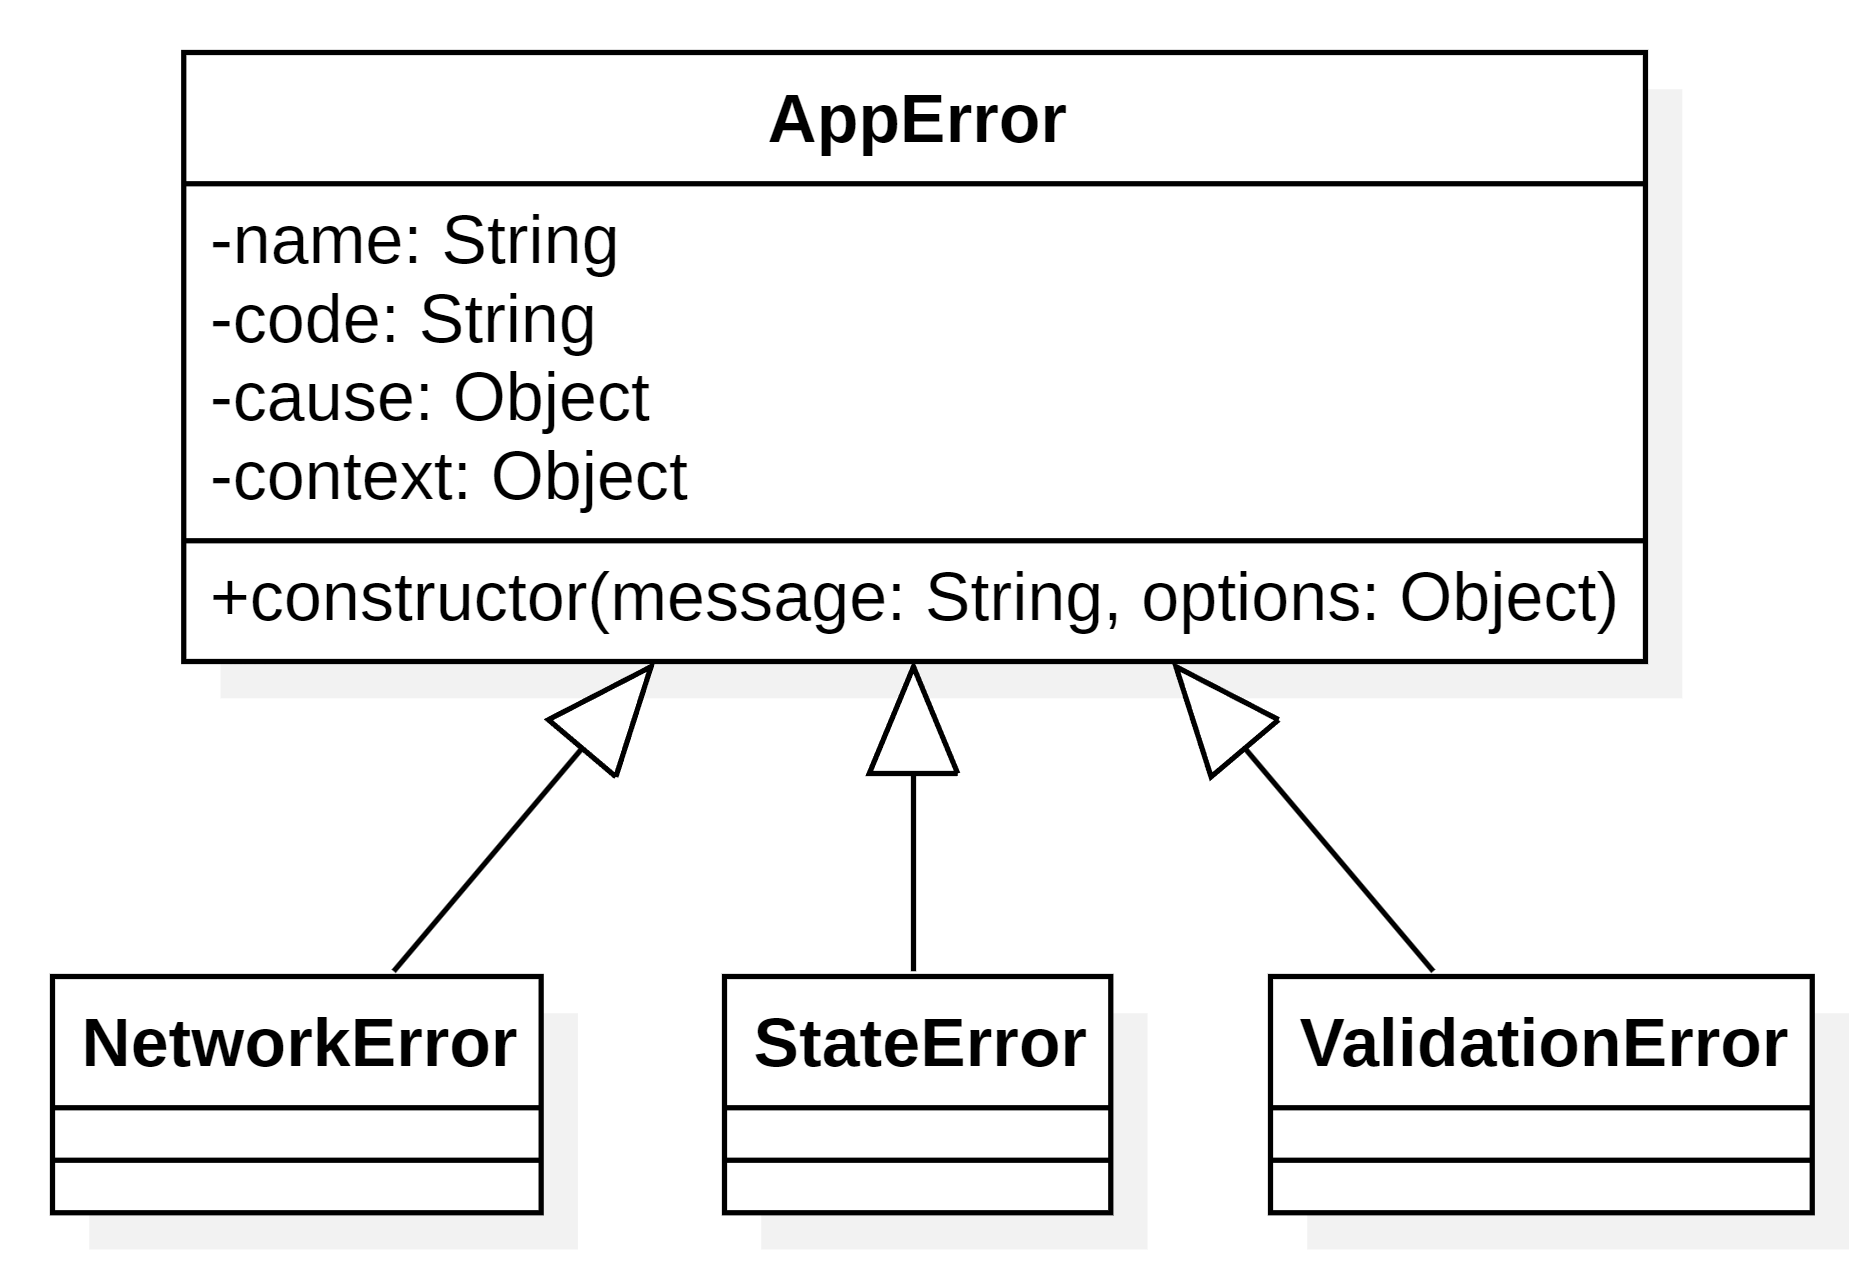
\includegraphics[width=.4\linewidth]{../../../Assets/classiFront/AppError.png}
                        \caption{Gerarchia errori application}
                    \end{figure}
                \end{center}
                Gerarchia di errori applicativi tipizzati per distinguere errori di rete, stato o validazione.\\\\
                \textbf{Attributi (AppError)}
                \begin{itemize}
                    \item {\ttfamily name}: nome della classe di \textit{errore}\textsubscript{\href{https://atlasteam9.github.io/Atlas/glossario.html\#Errore}{G}};
                    \item {\ttfamily code}: codice applicativo dell'\textit{errore}\textsubscript{\href{https://atlasteam9.github.io/Atlas/glossario.html\#Errore}{G}};
                    \item {\ttfamily cause}: eventuale \textit{errore}\textsubscript{\href{https://atlasteam9.github.io/Atlas/glossario.html\#Errore}{G}} origine;
                    \item {\ttfamily context}: contesto aggiuntivo per debug/logging.
                \end{itemize}
                \textbf{Metodi}
                \begin{itemize}
                    \item {\ttfamily constructor(message, options)}: inizializza l'\textit{errore}\textsubscript{\href{https://atlasteam9.github.io/Atlas/glossario.html\#Errore}{G}} base con metadati.
                \end{itemize}
                \textbf{Sottoclassi}
                \begin{itemize}
                    \item {\ttfamily NetworkError}: \textit{errore}\textsubscript{\href{https://atlasteam9.github.io/Atlas/glossario.html\#Errore}{G}} di comunicazione con backend;
                    \item {\ttfamily StateError}: \textit{errore}\textsubscript{\href{https://atlasteam9.github.io/Atlas/glossario.html\#Errore}{G}} di stato applicativo non coerente;
                    \item {\ttfamily ValidationError}: \textit{errore}\textsubscript{\href{https://atlasteam9.github.io/Atlas/glossario.html\#Errore}{G}} di \textit{validazione}\textsubscript{\href{https://atlasteam9.github.io/Atlas/glossario.html\#Validazione}{G}} input/dati.
                \end{itemize}

            % DESCRIZIONE HOOK FRONTEND 
            \paragraph{Custom Hooks}\mbox{}\\
                I custom hooks creati verranno di seguito descritti specificando ove presenti: i parametri dell'hook, le dipendenze esterne, lo stato interno locale, il comportamento e i valori esposti dall'hook.\\
                \subparagraph{useTreeBootstrap}\mbox{}\\
                Hook di bootstrap incaricato di caricare i {\ttfamily DecisionTree} all'avvio della sessione e di gestire la notifica di eventuali fallimenti del caricamento.\\\\
                \textbf{Parametri}
                \begin{itemize}
                    \item Nessuno.
                \end{itemize}
                \textbf{Dipendenze}
                \begin{itemize}
                    \item {\ttfamily TreeService}: utilizzato per invocare la logica di caricamento asincrono;
                    \item {\ttfamily notificationService}: ottenuto tramite il contesto applicativo ({\ttfamily useAppServices}) per la gestione dei feedback di errore.
                \end{itemize}
                \textbf{Stato interno}
                \begin{itemize}
                    \item Nessuno.
                \end{itemize}
                \textbf{Comportamento}
                \begin{itemize}
                    \item Esegue all'interno di un {\ttfamily useEffect} il metodo {\ttfamily TreeService.loadTrees()} al montaggio del componente o alla variazione del servizio di notifica;
                    \item Intercetta eventuali errori della {\ttfamily Promise} tramite {\ttfamily .catch()}, invocando \newline {\ttfamily notificationService.notifyError} con l'identificativo specifico {\ttfamily 'LOAD\_TREES\_ERROR'}.
                \end{itemize}
                
                \subparagraph{useSessionState}\mbox{}\\
                Hook di sola lettura delegato all'estrazione dello snapshot dello stato di sessione per la visualizzazione nella UI. Si \textit{interfaccia}\textsubscript{\href{https://atlasteam9.github.io/Atlas/glossario.html\#Interfaccia}{G}} direttamente con lo store globale per garantire una lettura reattiva dei dati senza l'intermediazione del livello di servizio.\\\\
                \textbf{Parametri}
                \begin{itemize}
                    \item Nessuno.
                \end{itemize}
                \textbf{Dipendenze}
                \begin{itemize}
                    \item {\ttfamily useSessionStore}: sorgente dati per lo stato della sessione;
                    \item {\ttfamily selectSessionStateSnapshot}: selettore incaricato di estrarre le proprietà rilevanti dal file di stato;
                    \item {\ttfamily useShallow}: utility di ottimizzazione fornita da Zustand.
                \end{itemize}
                \textbf{Stato interno}
                \begin{itemize}
                    \item Nessuno.
                \end{itemize}
                \textbf{Comportamento}
                \begin{itemize}
                    \item Restituisce l'insieme sincronizzato dei dati di sessione (identificativo, \textit{nodo}\textsubscript{\href{https://atlasteam9.github.io/Atlas/glossario.html\#Nodo}{G}} corrente, indici di posizione e cronologia delle risposte);
                    \item Implementa una strategia di aggiornamento efficiente tramite {\ttfamily useShallow}, che esegue una comparazione superficiale dei dati restituiti dal selettore per evitare aggiornamenti superflui del componente React.
                \end{itemize}
                
                \subparagraph{useSessionHandlers}\mbox{}\\
                Hook orchestratore che genera dinamicamente gli handler asincroni per le azioni della sessione (navigazione, risposte, salvataggio), centralizzando la gestione dello stato di caricamento e la cattura degli errori.\\\\
                \textbf{Parametri}
                \begin{itemize}
                    \item Nessuno.
                \end{itemize}
                \textbf{Dipendenze}
                \begin{itemize}
                    \item {\ttfamily navigate} (React \textit{Router}\textsubscript{\href{https://atlasteam9.github.io/Atlas/glossario.html\#Router}{G}}): per il reindirizzamento post azione;
                    \item {\ttfamily UIStore}: per la sincronizzazione globale del flag {\ttfamily isLoading};
                    \item {\ttfamily sessionHandlersConfig}: fornisce le definizioni atomiche delle azioni;
                    \item {\ttfamily createAsyncHandler}: factory per l'iniezione di logica trasversale (loading/error) negli handler.
                \end{itemize}
                \textbf{Stato interno}
                \begin{itemize}
                    \item {\ttfamily error}: memorizza l'ultimo \textit{errore}\textsubscript{\href{https://atlasteam9.github.io/Atlas/glossario.html\#Errore}{G}} intercettato durante un'azione asincrona.
                \end{itemize}
                \textbf{Comportamento}
                \begin{itemize}
                    \item Utilizza {\ttfamily useMemo} per generare una mappa di funzioni ({\ttfamily actionHandlers}) riducendo le configurazioni ottenute da {\ttfamily getHandlerConfigs};
                    \item Ogni handler generato automatizza il ciclo di vita dell'azione: attivazione del loading globale, esecuzione della logica, gestione del successo e gestione centralizzata dell'errore.
                \end{itemize}
                \textbf{Valori esposti}
                \begin{itemize}
                    \item {\ttfamily ...actionHandlers}: set di funzioni pronte per l'uso nella \textit{UI}\textsubscript{\href{https://atlasteam9.github.io/Atlas/glossario.html\#UI}{G}} (es. {\ttfamily handleYesClick}, {\ttfamily handleSaveAndExitClick});
                    \item {\ttfamily isLoading}: stato di caricamento globale derivato dal selettore dello store;
                    \item {\ttfamily error}: riferimento all'\textit{errore}\textsubscript{\href{https://atlasteam9.github.io/Atlas/glossario.html\#Errore}{G}} locale per la visualizzazione di feedback immediati nel runner.
                \end{itemize}
                
                \subparagraph{useSessionRedirect}\mbox{}\\
                Hook di guardia utilizzato per proteggere le pagine del runner. Verifica la presenza di sessione o dispositivo corrente e, in caso di assenza, esegue un reindirizzamento forzato.\\\\
                \textbf{Parametri}
                \begin{itemize}
                    \item {\ttfamily sessionId}: identificativo della sessione corrente;
                    \item {\ttfamily currentDevice}: oggetto rappresentante il dispositivo corrente.
                \end{itemize}
                \textbf{Dipendenze}
                \begin{itemize}
                    \item {\ttfamily navigate} ({\ttfamily useNavigate} di React \textit{Router}\textsubscript{\href{https://atlasteam9.github.io/Atlas/glossario.html\#Router}{G}}): utilizzato per il reindirizzamento.
                \end{itemize}
                \textbf{Stato interno}
                \begin{itemize}
                    \item Nessuno.
                \end{itemize}
                \textbf{Comportamento}
                \begin{itemize}
                    \item All'interno di un {\ttfamily useEffect}, verifica se uno dei parametri ({\ttfamily sessionId} o {\ttfamily currentDevice}) risulti nullo o non definito;
                    \item In caso di mancata conformità alle precondizioni, esegue il reindirizzamento alla rotta di riepilogo del dispositivo ({\ttfamily /device/summary}).
                \end{itemize}
                
                \subparagraph{useResultViewLogic}\mbox{}\\
                Hook orchestratore della logica di presentazione della vista risultati. Centralizza l'accesso ai dati di sessione, lo stato dei risultati e le funzionalità di \textit{esportazione}\textsubscript{\href{https://atlasteam9.github.io/Atlas/glossario.html\#Esportazione}{G}} e navigazione.\\\\
                \textbf{Parametri}
                \begin{itemize}
                    \item Nessuno.
                \end{itemize}
                \textbf{Dipendenze}
                \begin{itemize}
                    \item {\ttfamily useResultStore} e {\ttfamily useSessionStore}: accesso allo stato globale;
                    \item {\ttfamily useCurrentDevice}: recupero del dispositivo in uso;
                    \item {\ttfamily useExportResults} e {\ttfamily useExportSession}: hook specializzati per le procedure di \textit{esportazione}\textsubscript{\href{https://atlasteam9.github.io/Atlas/glossario.html\#Esportazione}{G}};
                    \item {\ttfamily resetSessionAndNavigateHome}: logica di terminazione sessione.
                \end{itemize}
                \textbf{Stato interno}
                \begin{itemize}
                    \item {\ttfamily expandedRequirement}: memorizza l'id del \textit{requisito}\textsubscript{\href{https://atlasteam9.github.io/Atlas/glossario.html\#Requisito}{G}} attualmente espanso nella \textit{UI}\textsubscript{\href{https://atlasteam9.github.io/Atlas/glossario.html\#UI}{G}} per visualizzarne i dettagli.
                \end{itemize}
                \textbf{Comportamento}
                \begin{itemize}
                    \item Gestisce la navigazione verso la prosecuzione del test, la modifica della sessione o il ritorno alla home;
                    \item Coordina l'apertura del dialogo di formattazione e l'avvio del download per i report (\textit{CSV}\textsubscript{\href{https://atlasteam9.github.io/Atlas/glossario.html\#CSV}{G}}, \textit{PDF}\textsubscript{\href{https://atlasteam9.github.io/Atlas/glossario.html\#PDF}{G}}) e per il backup della sessione (JSON);
                    \item Implementa il toggle visivo per l'espansione dei singoli requisiti nella \textit{lista}\textsubscript{\href{https://atlasteam9.github.io/Atlas/glossario.html\#Lista}{G}} dei risultati.
                \end{itemize}
                \textbf{Valori esposti}
                \begin{itemize}
                    \item Dati: {\ttfamily results}, {\ttfamily device}, {\ttfamily resultsPerAsset};
                    \item Flag di stato: {\ttfamily isTestFinished}, {\ttfamily isSessionUploaded}, {\ttfamily isExporting}, ecc.;
                    \item Handler: metodi per la navigazione, il toggle della \textit{UI}\textsubscript{\href{https://atlasteam9.github.io/Atlas/glossario.html\#UI}{G}} e l'esecuzione degli export.
                \end{itemize}
                
                \subparagraph{useModifySessionLogic}\mbox{}\\
                Hook orchestratore per la logica di modifica della sessione. Gestisce il filtraggio dei risultati modificabili, la selezione dei target di ripresa (asset/requisito) e il ripristino dello stato applicativo per la riesecuzione dei test.\\\\
                \textbf{Parametri}
                \begin{itemize}
                    \item Nessuno.
                \end{itemize}
                \textbf{Dipendenze}
                \begin{itemize}
                    \item {\ttfamily useResultStore}, {\ttfamily useTreeStore}, {\ttfamily useDeviceStore}, {\ttfamily useSessionStore}: accesso centralizzato allo stato globale;
                    \item {\ttfamily filterResumableResults}: logica di dominio per identificare i requisiti che supportano la ripresa;
                    \item {\ttfamily sessionService}: per l'esecuzione della logica di {\ttfamily resume};
                    \item {\ttfamily useNavigate}: per la navigazione programmatica verso il runner o i risultati.
                \end{itemize}
                \textbf{Stato interno}
                \begin{itemize}
                    \item {\ttfamily expandedRequirement}: ID del \textit{requisito}\textsubscript{\href{https://atlasteam9.github.io/Atlas/glossario.html\#Requisito}{G}} attualmente espanso nella \textit{lista}\textsubscript{\href{https://atlasteam9.github.io/Atlas/glossario.html\#Lista}{G}};
                    \item {\ttfamily selectedAsset}: ID dell'asset selezionato all'interno del \textit{requisito}\textsubscript{\href{https://atlasteam9.github.io/Atlas/glossario.html\#Requisito}{G}} espanso per l'operazione di {\ttfamily resume}.
                \end{itemize}
                \textbf{Comportamento}
                \begin{itemize}
                    \item Filtraggio: calcola in modo ottimizzato ({\ttfamily useMemo}) i risultati che possono essere ripresi basandosi sulle regole di dominio;
                    \item Selezione: gestisce il toggle della \textit{UI}\textsubscript{\href{https://atlasteam9.github.io/Atlas/glossario.html\#UI}{G}} per i requisiti e la selezione esclusiva di un asset per il riavvio;
                    \item Ripresa test: verifica la validità della selezione e invoca {\ttfamily sessionService.resumeSession} per ricalibrare la storia e la posizione della sessione prima di navigare al runner;
                    \item Navigazione: fornisce un handler dedicato per il ritorno alla vista dei risultati.
                \end{itemize}
                \textbf{Valori esposti}
                \begin{itemize}
                    \item Dati filtrati: {\ttfamily filteredResults}, {\ttfamily dependenciesByRequirement};
                    \item Stato \textit{UI}\textsubscript{\href{https://atlasteam9.github.io/Atlas/glossario.html\#UI}{G}}: {\ttfamily expandedRequirement}, {\ttfamily selectedAsset};
                    \item Contesto: {\ttfamily resultsPerAsset}, {\ttfamily device};
                    \item Azioni: {\ttfamily handleToggleRequirement}, {\ttfamily handleSelectAsset}, {\ttfamily handleResumeTest}, {\ttfamily handleBack}.
                \end{itemize}
                
                \subparagraph{useAssetManagement}\mbox{}\\
                Hook orchestratore per la vista di gestione degli asset. Coordina le operazioni di modifica del dispositivo (aggiunta/rimozione asset), il salvataggio su file e la logica di guardia per il passaggio alla sessione di test in presenza di modifiche non salvate.\\\\
                \textbf{Parametri}
                \begin{itemize}
                    \item Nessuno.
                \end{itemize}
                \textbf{Dipendenze}
                \begin{itemize}
                    \item {\ttfamily useNavigate}: per la navigazione verso la creazione asset o il riepilogo del dispositivo;
                    \item {\ttfamily SessionService}: utilizzato per inizializzare la sessione a partire dal dispositivo corrente;
                    \item {\ttfamily DeviceService}: per le operazioni di persistenza (salvataggio su file) e rimozione asset;
                    \item {\ttfamily notificationService}: per la segnalazione di errori durante la creazione della sessione;
                    \item {\ttfamily UIStore}: per il monitoraggio dello stato {\ttfamily isDirty} (presenza di modifiche non salvate).
                \end{itemize}
                \textbf{Stato interno}
                \begin{itemize}
                    \item {\ttfamily showUnsavedDialog}: booleano che controlla la visibilità del dialog di conferma per le modifiche non salvate.
                \end{itemize}
                \textbf{Comportamento}
                \begin{itemize}
                    \item Gestione asset: fornisce handler per la navigazione verso la creazione di nuovi asset e delega la rimozione a {\ttfamily DeviceService};
                    \item Logica di guardia: in {\ttfamily onGoToSummary}, verifica se il dispositivo ha modifiche pendenti tramite {\ttfamily isDirty}. Se presente, attiva il dialog di avviso; in caso contrario, procede alla creazione della sessione;
                    \item Persistenza e navigazione: coordina il salvataggio del dispositivo prima del passaggio al riepilogo ({\ttfamily onConfirmSaveBeforeSummary}) o permette il proseguimento ignorando le modifiche;
                    \item Creazione sessione: incapsula la chiamata asincrona a \newline {\ttfamily sessionService.createSessionWithDevice} gestendo il feedback in caso di errore.
                \end{itemize}
                \textbf{Valori esposti}
                \begin{itemize}
                    \item {\ttfamily currentDevice}: riferimento al dispositivo attualmente in gestione;
                    \item {\ttfamily showUnsavedDialog}: stato visivo per la \textit{UI}\textsubscript{\href{https://atlasteam9.github.io/Atlas/glossario.html\#UI}{G}};
                    \item \textit{Interfaccia}\textsubscript{\href{https://atlasteam9.github.io/Atlas/glossario.html\#Interfaccia}{G}} dei metodi: set completo di handler per la manipolazione degli asset, la navigazione e il controllo del flusso di salvataggio.
                \end{itemize}
                
                \subparagraph{useHomeNavigation}\mbox{}\\
                Hook orchestratore della pagina iniziale ({\ttfamily HomeView}) che centralizza i flussi di ingresso principali dell'applicazione. Gestisce l'inizializzazione dell'\textit{ambiente di lavoro}\textsubscript{\href{https://atlasteam9.github.io/Atlas/glossario.html\#Ambientedilavoro}{G}} attraverso il caricamento di configurazioni esistenti (dispositivi o sessioni) o la creazione di nuovi asset.\\\\
                \textbf{Parametri}
                \begin{itemize}
                    \item Nessuno.
                \end{itemize}
                \textbf{Dipendenze}
                \begin{itemize}
                    \item {\ttfamily useNavigate} (React \textit{Router}\textsubscript{\href{https://atlasteam9.github.io/Atlas/glossario.html\#Router}{G}}): per il reindirizzamento programmatico alle diverse sezioni dell'app;
                    \item {\ttfamily SessionService}: per l'interazione con le \textit{API}\textsubscript{\href{https://atlasteam9.github.io/Atlas/glossario.html\#API}{G}} di backend relative alla creazione e al ripristino delle sessioni;
                    \item {\ttfamily notificationService}: per la gestione e visualizzazione degli errori durante le operazioni di I/O, ottenuto tramite contesto applicativo.
                \end{itemize}
                \textbf{Stato interno}
                \begin{itemize}
                    \item Nessuno (delega la persistenza dello stato agli store globali tramite i \textit{servizi}\textsubscript{\href{https://atlasteam9.github.io/Atlas/glossario.html\#Servizi}{G}}).
                \end{itemize}
                \textbf{Comportamento}
                \begin{itemize}
                    \item {\ttfamily handleLoadDevice(file)}: coordina l'invocazione asincrona di \newline {\ttfamily SessionService.createSessionWithFile(file)}. In caso di successo, l'utente viene indirizzato alla pagina di riepilogo del dispositivo;
                    \item {\ttfamily handleCreateDevice()}: gestisce la navigazione verso l'\textit{interfaccia}\textsubscript{\href{https://atlasteam9.github.io/Atlas/glossario.html\#Interfaccia}{G}} di creazione manuale di un nuovo dispositivo;
                    \item {\ttfamily handleLoadPreviousSession(file)}: esegue il ripristino di una sessione salvata tramite {\ttfamily SessionService.loadSessionFromFile(file)}, automatizzando il caricamento della cronologia e navigando direttamente alla vista dei risultati finali.
                \end{itemize}
                \textbf{Valori esposti}
                \begin{itemize}
                    \item Set di handler per le azioni principali della dashboard iniziale.
                \end{itemize}
                
                \subparagraph{useRouteGuardAccess}\mbox{}\\
                Hook di autorizzazione per il sistema di routing che determina se una rotta protetta è accessibile sulla base dello stato corrente della sessione e del dispositivo.\\\\
                \textbf{Parametri}
                \begin{itemize}
                    \item {\ttfamily routeConfig}: oggetto di configurazione della rotta che definisce se il percorso è protetto ({\ttfamily isProtected}) e se richiede esplicitamente un identificativo di sessione ({\ttfamily requiresSessionId}).
                \end{itemize}
                \textbf{Dipendenze}
                \begin{itemize}
                    \item {\ttfamily useSessionStore}: utilizzato per monitorare il {\ttfamily sessionId} corrente;
                    \item {\ttfamily useDeviceStore}: utilizzato per monitorare il {\ttfamily currentDevice};
                    \item {\ttfamily selectRouteAccess}: selettore composito che incapsula la logica di \textit{validazione}\textsubscript{\href{https://atlasteam9.github.io/Atlas/glossario.html\#Validazione}{G}} dei criteri di accesso.
                \end{itemize}
                \textbf{Stato interno}
                \begin{itemize}
                    \item Nessuno.
                \end{itemize}
                \textbf{Comportamento}
                \begin{itemize}
                    \item Utilizza {\ttfamily useMemo} per ottimizzare le prestazioni, ricalcolando il permesso di accesso solo al variare della configurazione della rotta, del dispositivo o della sessione;
                    \item Se la rotta non è contrassegnata come protetta, l'accesso è garantito in modo predefinito ({\ttfamily true});
                    \item In caso di rotta protetta, determina se la sessione è obbligatoria (default {\ttfamily true} a meno di specifica contraria) e delega la valutazione finale a {\ttfamily selectRouteAccess}.
                \end{itemize}
                \textbf{Valori esposti}
                \begin{itemize}
                    \item Un valore booleano che indica la legittimità dell'accesso alla rotta configurata.
                \end{itemize}

                \subparagraph{useExportResults}\mbox{}\\
                Hook specializzato nella gestione del flusso di \textit{esportazione}\textsubscript{\href{https://atlasteam9.github.io/Atlas/glossario.html\#Esportazione}{G}} dei risultati aggregati, includendo selezione del formato, stato di avanzamento e gestione errori.\\\\
                \textbf{Parametri}
                \begin{itemize}
                    \item {\ttfamily sessionId}: identificativo della sessione per cui esportare i risultati.
                \end{itemize}
                \textbf{Dipendenze}
                \begin{itemize}
                    \item {\ttfamily ExportService}: esecuzione export in formato CSV/PDF;
                    \item {\ttfamily notificationService}: notifica errori utente;
                    \item {\ttfamily UIStore}: gestione del flag globale {\ttfamily isExporting}.
                \end{itemize}
                \textbf{Stato interno}
                \begin{itemize}
                    \item {\ttfamily showFormatDialog}: controlla la visibilità del dialogo di scelta formato.
                \end{itemize}
                \textbf{Comportamento}
                \begin{itemize}
                    \item {\ttfamily handleExportClick()} apre il dialogo di selezione formato;
                    \item {\ttfamily handleExportFormat(format)} chiude il dialogo, abilita il flag di export, invoca il metodo di export coerente col formato e gestisce eventuali errori con notifica;
                    \item al termine dell'operazione resetta sempre il flag di export.
                \end{itemize}
                \textbf{Valori esposti}
                \begin{itemize}
                    \item {\ttfamily isExporting};
                    \item {\ttfamily showFormatDialog};
                    \item {\ttfamily handleExportClick}, {\ttfamily handleExportFormat}, {\ttfamily setShowFormatDialog}.
                \end{itemize}

                \subparagraph{useExportSession}\mbox{}\\
                Hook dedicato all'\textit{esportazione}\textsubscript{\href{https://atlasteam9.github.io/Atlas/glossario.html\#Esportazione}{G}} completa della sessione corrente in formato JSON, con gestione uniforme dello stato di avanzamento e degli errori.\\\\
                \textbf{Parametri}
                \begin{itemize}
                    \item {\ttfamily sessionId}: identificativo della sessione da esportare.
                \end{itemize}
                \textbf{Dipendenze}
                \begin{itemize}
                    \item {\ttfamily SessionService}: recupero risposte formattate;
                    \item {\ttfamily ExportService}: \textit{esportazione}\textsubscript{\href{https://atlasteam9.github.io/Atlas/glossario.html\#Esportazione}{G}} JSON della sessione;
                    \item {\ttfamily notificationService}: notifica errori;
                    \item {\ttfamily UIStore}: gestione del flag {\ttfamily isExportingSession}.
                \end{itemize}
                \textbf{Stato interno}
                \begin{itemize}
                    \item Nessuno.
                \end{itemize}
                \textbf{Comportamento}
                \begin{itemize}
                    \item {\ttfamily handleExportSessionClick()} attiva il flag di export sessione, costruisce il payload risposte tramite servizio di sessione, avvia l'export e notifica eventuali errori;
                    \item in ogni caso disattiva il flag di export al termine.
                \end{itemize}
                \textbf{Valori esposti}
                \begin{itemize}
                    \item {\ttfamily isExportingSession};
                    \item {\ttfamily handleExportSessionClick}.
                \end{itemize}
                
                \subparagraph{useSessionRunnerTrees}\mbox{}\\
                Hook di lettura che espone i \textit{decision tree}\textsubscript{\href{https://atlasteam9.github.io/Atlas/glossario.html\#DecisionTree}{G}} necessari alla \textit{UI}\textsubscript{\href{https://atlasteam9.github.io/Atlas/glossario.html\#UI}{G}} del runner, delegando l'accesso allo stato globale tramite selector composito.\\\\
                \textbf{Parametri}
                \begin{itemize}
                    \item Nessuno.
                \end{itemize}
                \textbf{Dipendenze}
                \begin{itemize}
                    \item {\ttfamily useTreeStore}: sorgente stato dei tree;
                    \item {\ttfamily selectSessionRunnerTrees}: selector composito per estrazione dati.
                \end{itemize}
                \textbf{Stato interno}
                \begin{itemize}
                    \item Nessuno.
                \end{itemize}
                \textbf{Comportamento}
                \begin{itemize}
                    \item Restituisce in modo reattivo i tree correnti necessari al flusso del Session Runner.
                \end{itemize}
                \textbf{Valori esposti}
                \begin{itemize}
                    \item \textit{Lista}\textsubscript{\href{https://atlasteam9.github.io/Atlas/glossario.html\#Lista}{G}} dei \textit{decision tree}\textsubscript{\href{https://atlasteam9.github.io/Atlas/glossario.html\#DecisionTree}{G}} correnti.
                \end{itemize}
                
                \subparagraph{useBeforeUnload}\mbox{}\\
                Hook di protezione lifecycle che gestisce la chiusura o ricarica della pagina, assicurando la terminazione della sessione lato backend e la pulizia dello stato locale.\\\\
                \textbf{Parametri}
                \begin{itemize}
                    \item Nessuno.
                \end{itemize}
                \textbf{Dipendenze}
                \begin{itemize}
                    \item {\ttfamily sessionService}: accesso a sessionId e operazioni di cleanup;
                    \item \textit{API}\textsubscript{\href{https://atlasteam9.github.io/Atlas/glossario.html\#API}{G}} browser {\ttfamily beforeunload} + chiamata {\ttfamily fetch} con {\ttfamily keepalive}.
                \end{itemize}
                \textbf{Stato interno}
                \begin{itemize}
                    \item Nessuno.
                \end{itemize}
                \textbf{Comportamento}
                \begin{itemize}
                    \item Registra un listener su {\ttfamily window.beforeunload};
                    \item se esiste una sessione attiva, invia una DELETE al backend con {\ttfamily keepalive: true};
                    \item invoca la pulizia locale della sessione;
                    \item alla dismissione del componente rimuove il listener registrato.
                \end{itemize}
                \textbf{Valori esposti}
                \begin{itemize}
                    \item Nessuno (hook a effetto collaterale).
                \end{itemize}

            % DESCRIZIONE STORE FRONTEND 
            \paragraph{Store e selectors}\mbox{}\\
            Per lo state management vengono descritti gli store specificando i loro attributi e il loro metodi.

                \subparagraph{SessionStore}\mbox{}\\
                \begin{center}
                    \begin{figure}[H]
                        \centering
                        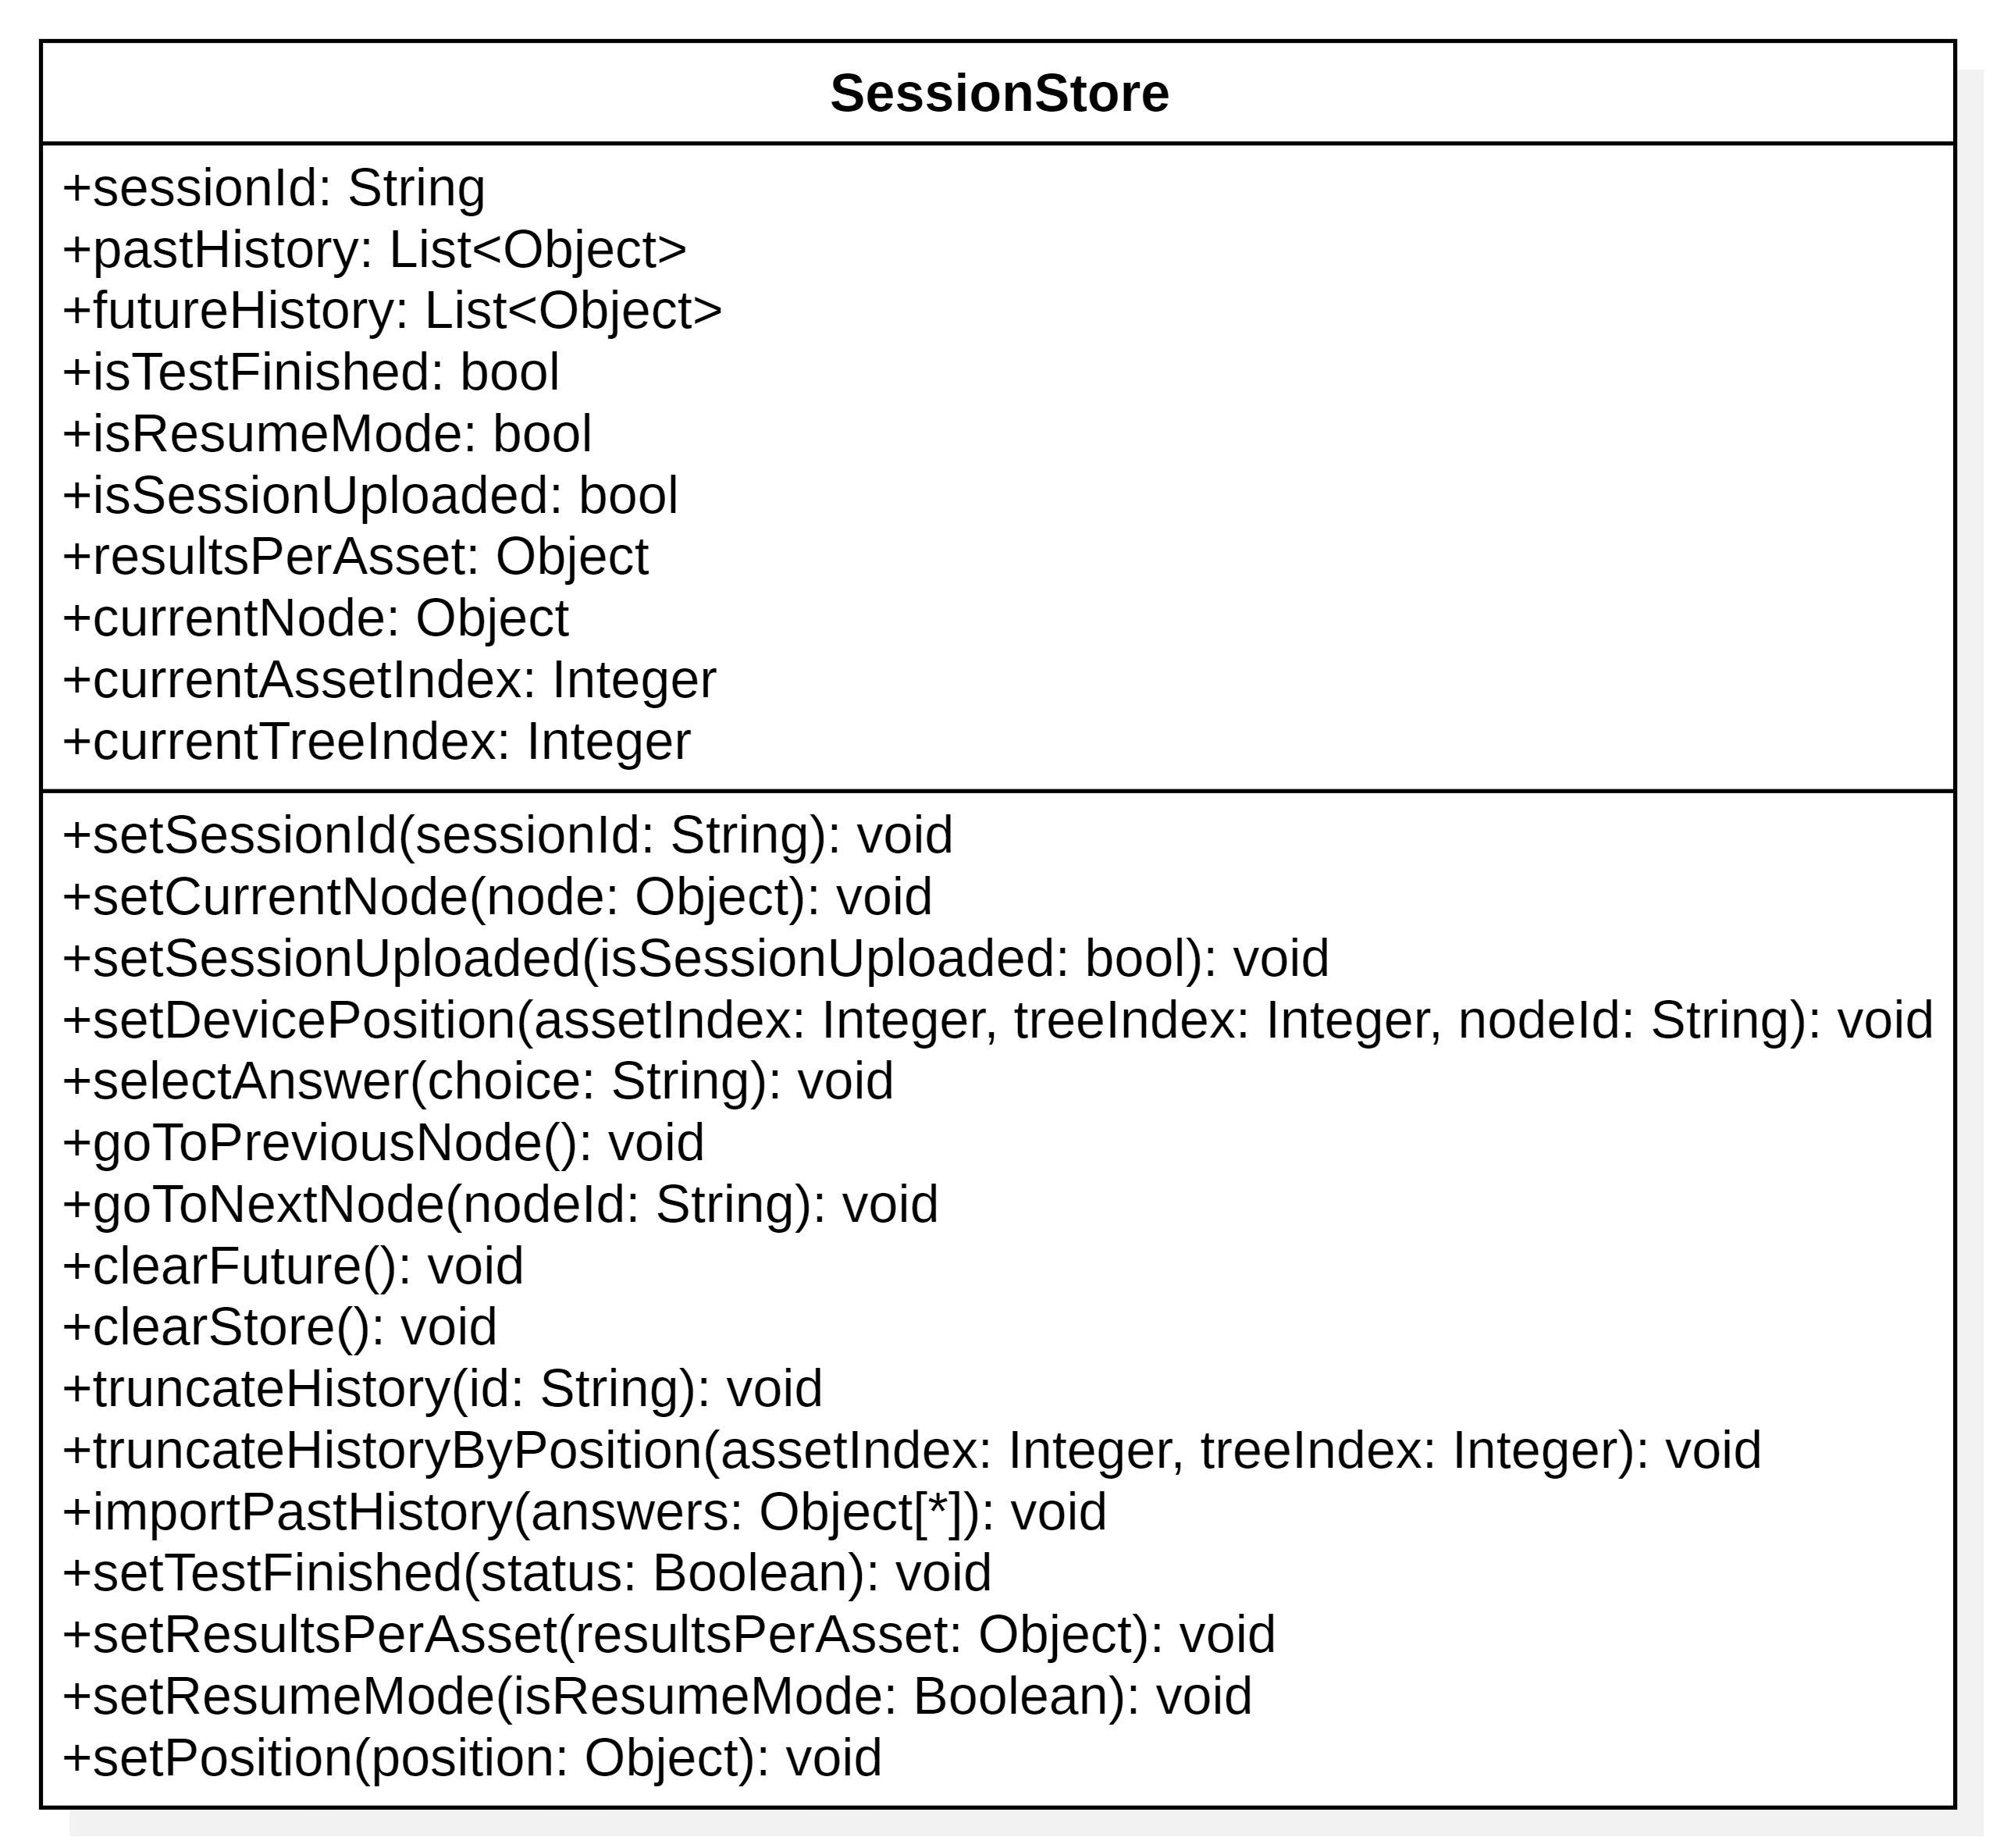
\includegraphics[width=.6\linewidth]{../../../Assets/classiFront/SessionStore.png}
                        \caption{SessionStore: store state management}
                    \end{figure}
                \end{center}
                Store principale per lo stato della sessione di test: posizione corrente, storico risposte, avanzamento e flag di flusso.\\\\
                \textbf{Attributi}
                \begin{itemize}
                    \item {\ttfamily sessionId}: identificativo sessione corrente;
                    \item {\ttfamily pastHistory}: storico delle risposte date dall'utente;
                    \item {\ttfamily futureHistory}: storico in avanti per navigazione;
                    \item {\ttfamily isTestFinished}: flag di completamento sessione;
                    \item {\ttfamily isResumeMode}: flag di ripresa da sessione modificata;
                    \item {\ttfamily isSessionUploaded}: indica se la sessione è caricata da file;
                    \item {\ttfamily resultsPerAsset}: risultati dettagliati per asset;
                    \item {\ttfamily currentNode}: riferimento al \textit{nodo}\textsubscript{\href{https://atlasteam9.github.io/Atlas/glossario.html\#Nodo}{G}} corrente;
                    \item {\ttfamily currentAssetIndex}, {\ttfamily currentTreeIndex}: posizione corrente su asset e requisito.
                \end{itemize}
                \textbf{Metodi}
                \begin{itemize}
                    \item Metodi setter base: {\ttfamily setSessionId}, {\ttfamily setCurrentNode}, {\ttfamily setSessionUploaded}, \newline {\ttfamily setDevicePosition};
                    \item Gestione risposte/storico: {\ttfamily selectAnswer}, {\ttfamily importPastHistory}, {\ttfamily truncateHistory}, \newline {\ttfamily truncateHistoryByPosition};
                    \item Navigazione: {\ttfamily goToPreviousNode}, {\ttfamily goToNextNode}, {\ttfamily clearFuture}, {\ttfamily setPosition};
                    \item Flag di processo: {\ttfamily setTestFinished}, {\ttfamily setResumeMode}, {\ttfamily setResultsPerAsset};
                    \item Reset completo: {\ttfamily clearStore()}.
                \end{itemize}
                
                \subparagraph{DeviceStore}\mbox{}\\
                \begin{center}
                    \begin{figure}[H]
                        \centering
                        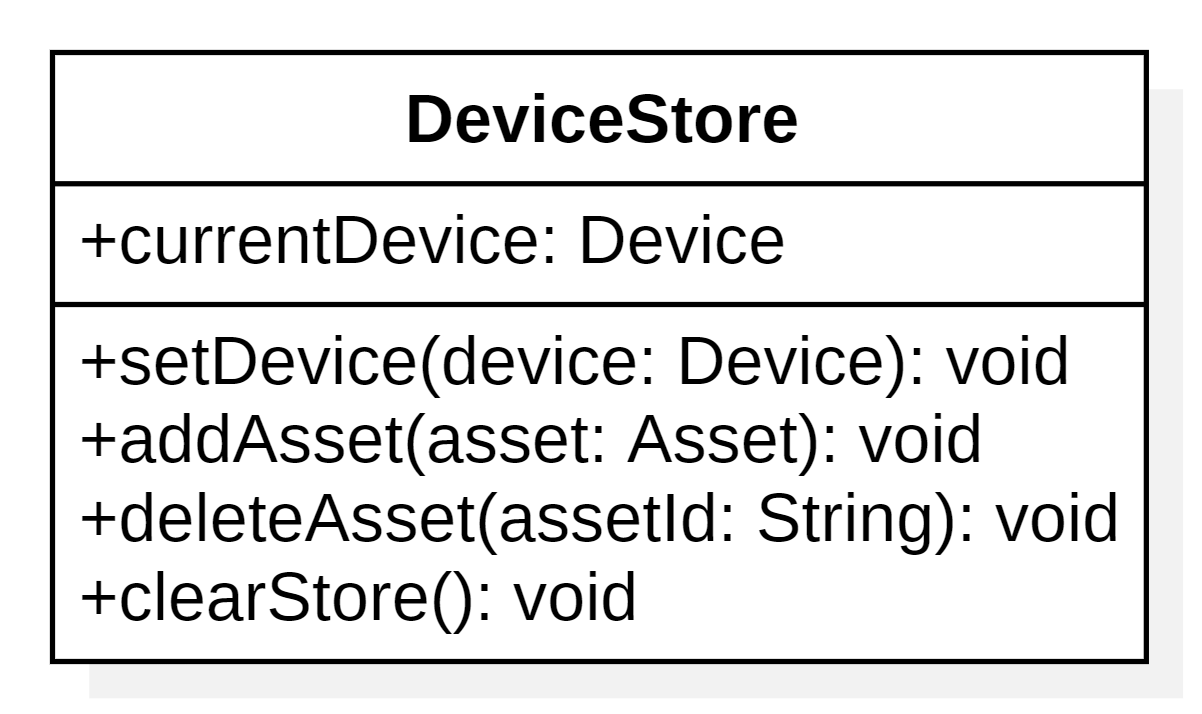
\includegraphics[width=.4\linewidth]{../../../Assets/classiFront/DeviceStore.png}
                        \caption{DeviceStore: store state management}
                    \end{figure}
                \end{center}
                Store dedicato al dispositivo corrente e alla sua \textit{lista}\textsubscript{\href{https://atlasteam9.github.io/Atlas/glossario.html\#Lista}{G}} di asset.\\\\
                \textbf{Attributi}
                \begin{itemize}
                    \item {\ttfamily currentDevice}: oggetto dispositivo attivo.
                \end{itemize}
                \textbf{Metodi}
                \begin{itemize}
                    \item {\ttfamily setDevice(device)}: imposta il dispositivo corrente;
                    \item {\ttfamily addAsset(asset)}: aggiunge un asset al dispositivo;
                    \item {\ttfamily deleteAsset(assetId)}: rimuove un asset dal dispositivo;
                    \item {\ttfamily clearStore()}: reset del dispositivo corrente.
                \end{itemize}
                
                \subparagraph{TreeStore}\mbox{}\\
                \begin{center}
                    \begin{figure}[H]
                        \centering
                        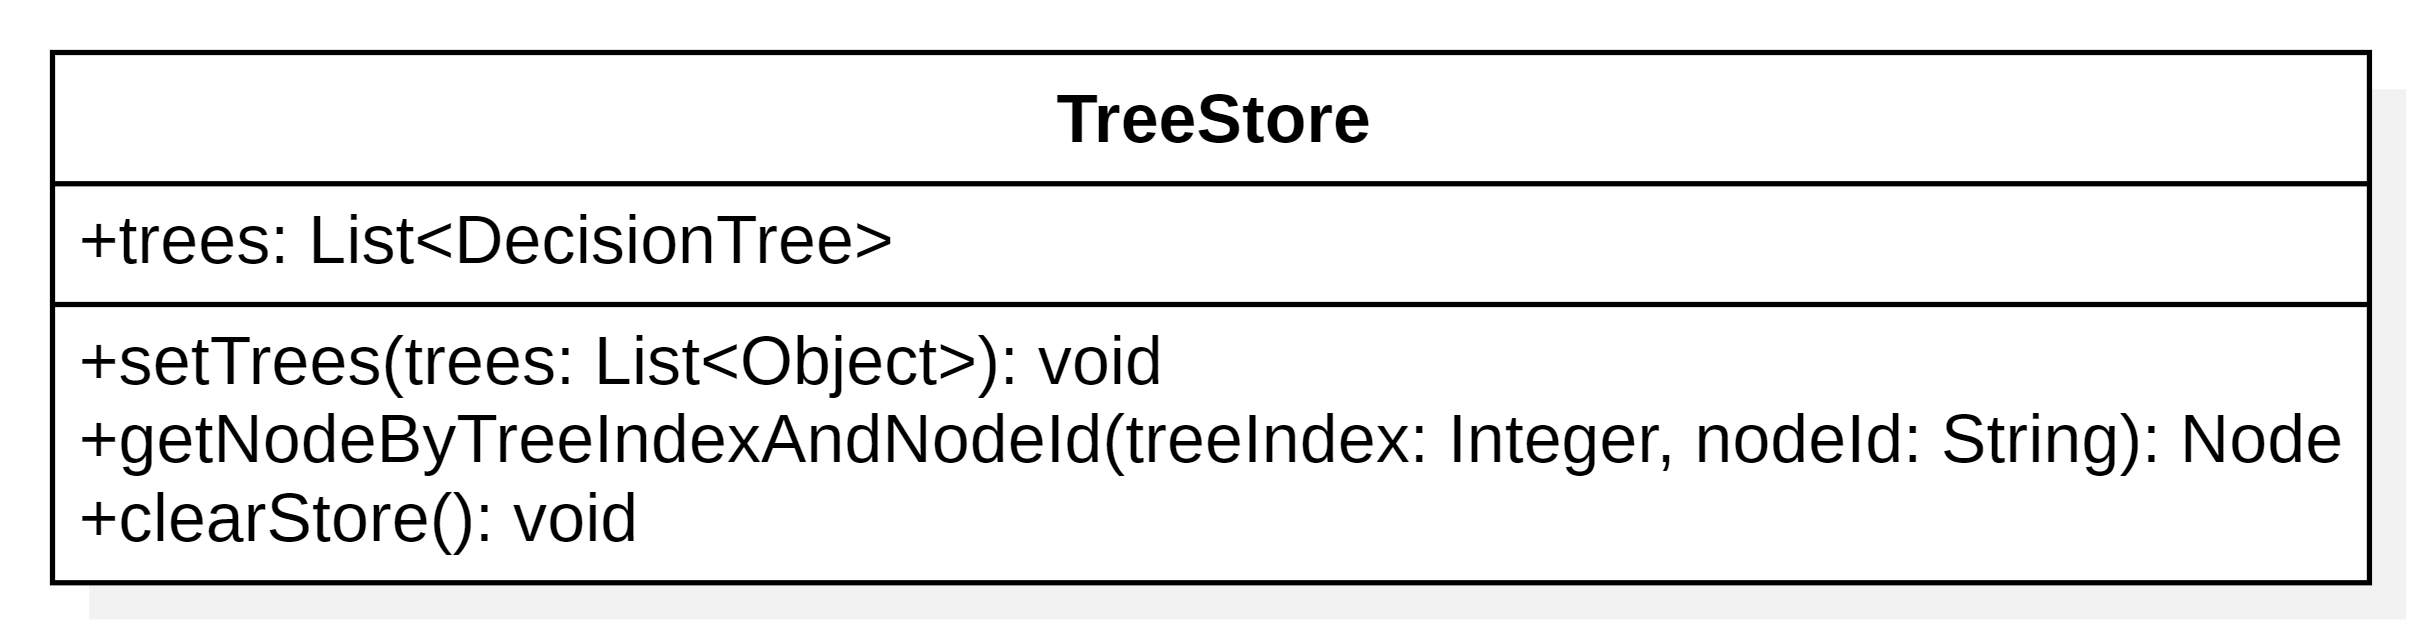
\includegraphics[width=.6\linewidth]{../../../Assets/classiFront/TreeStore.png}
                        \caption{TreeStore: store state management}
                    \end{figure}
                \end{center}
                Store dei \textit{decision tree}\textsubscript{\href{https://atlasteam9.github.io/Atlas/glossario.html\#DecisionTree}{G}} normalizzati usati durante il questionario.\\\\
                \textbf{Attributi}
                \begin{itemize}
                    \item {\ttfamily trees}: \textit{lista}\textsubscript{\href{https://atlasteam9.github.io/Atlas/glossario.html\#Lista}{G}} dei \textit{decision tree}\textsubscript{\href{https://atlasteam9.github.io/Atlas/glossario.html\#DecisionTree}{G}} caricati.
                \end{itemize}
                \textbf{Metodi}
                \begin{itemize}
                    \item {\ttfamily setTrees(trees)}: normalizza e salva i tree (anche da payload \textit{API}\textsubscript{\href{https://atlasteam9.github.io/Atlas/glossario.html\#API}{G}});
                    \item {\ttfamily getNodeByTreeIndexAndNodeId(treeIndex, nodeId)}: recupera un \textit{nodo}\textsubscript{\href{https://atlasteam9.github.io/Atlas/glossario.html\#Nodo}{G}} specifico del tree di indice {\ttfamily treeIndex};
                    \item {\ttfamily clearStore()}: reset della \textit{lista}\textsubscript{\href{https://atlasteam9.github.io/Atlas/glossario.html\#Lista}{G}} tree.
                \end{itemize}
                
                \subparagraph{ResultStore}\mbox{}\\
                \begin{center}
                    \begin{figure}[H]
                        \centering
                        
\includegraphics[width=.4\linewidth]{../../../Assets/classiFront/ResultStore.png}
                        \caption{ResultStore: store state management}
                    \end{figure}
                \end{center}
                Store dedicato ai risultati aggregati della sessione.\\\\
                \textbf{Attributi}
                \begin{itemize}
                    \item {\ttfamily results}: \textit{lista}\textsubscript{\href{https://atlasteam9.github.io/Atlas/glossario.html\#Lista}{G}} risultati aggregati per requisito.
                \end{itemize}
                \textbf{Metodi}
                \begin{itemize}
                    \item {\ttfamily setResults(results)}: aggiorna i risultati aggregati;
                    \item {\ttfamily clearStore()}: reset dei risultati.
                \end{itemize}
                
                \subparagraph{UIStore}\mbox{}\\
                \begin{center}
                    \begin{figure}[H]
                        \centering
                        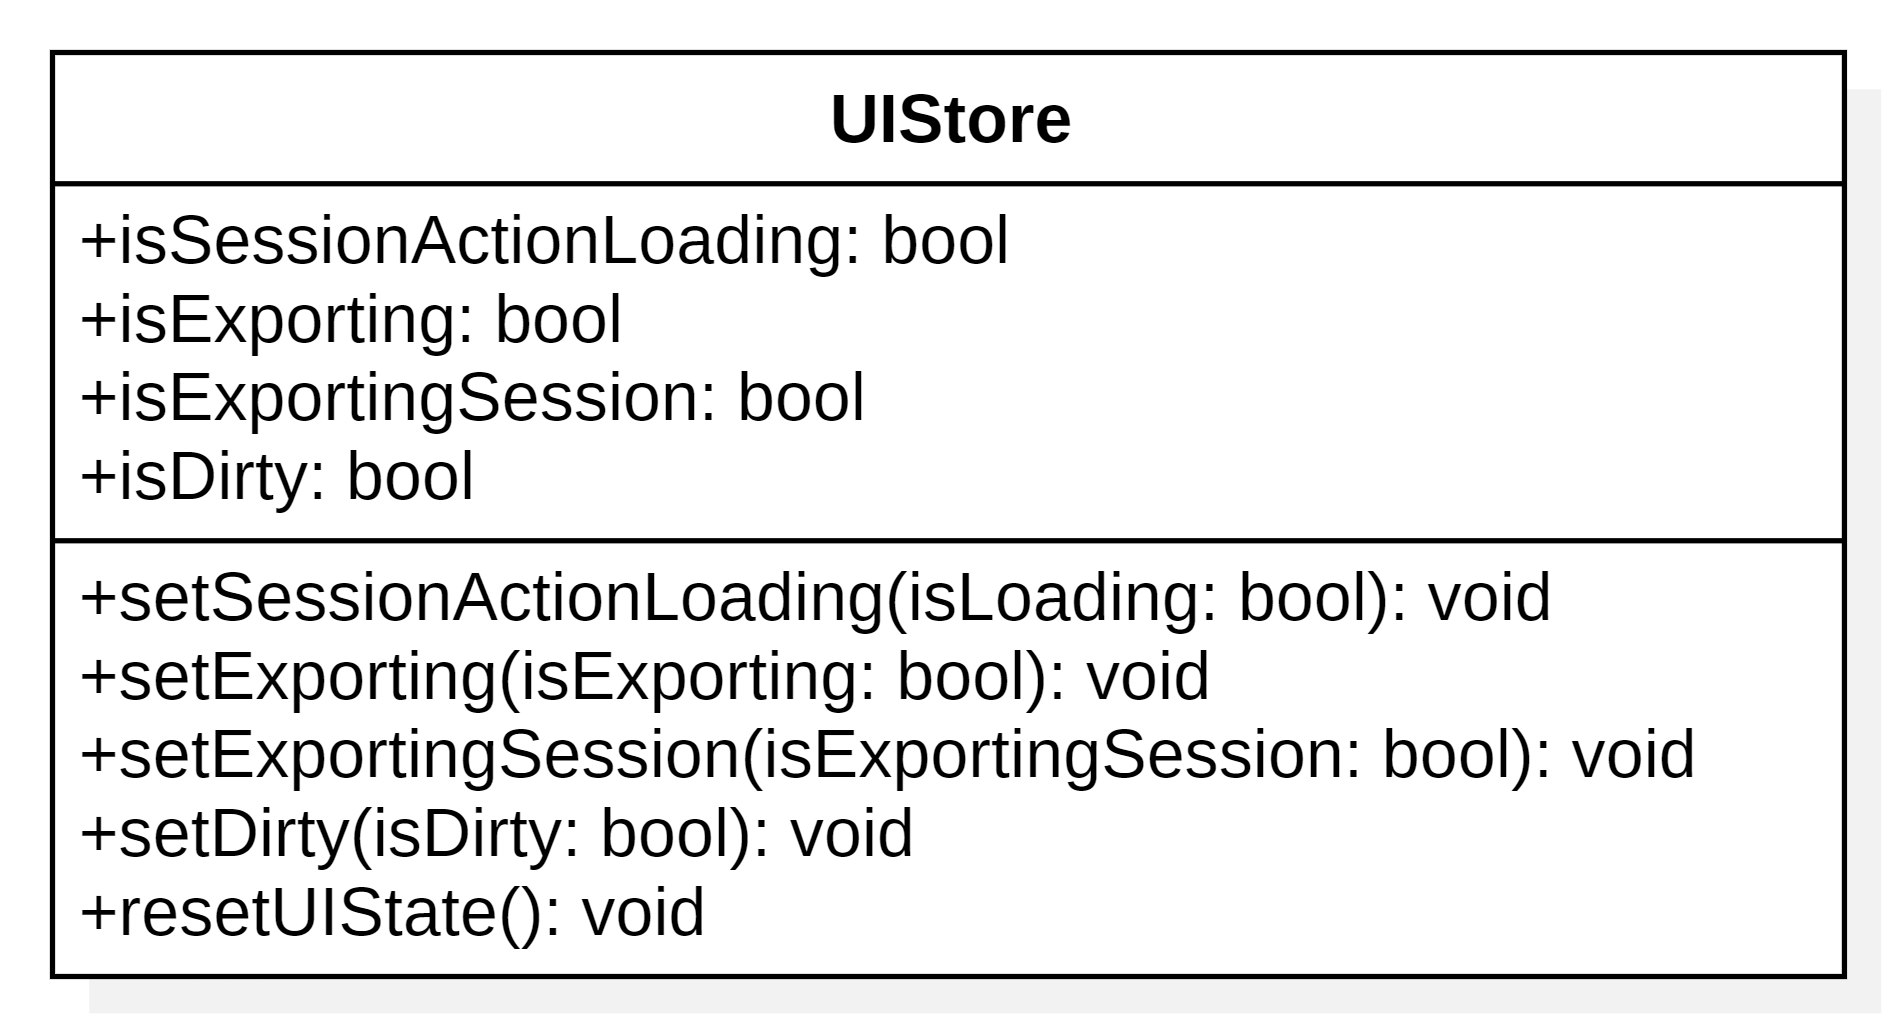
\includegraphics[width=.5\linewidth]{../../../Assets/classiFront/UIStore.png}
                        \caption{UIStore: store state management}
                    \end{figure}
                \end{center}
                Store trasversale per i flag \textit{UI}\textsubscript{\href{https://atlasteam9.github.io/Atlas/glossario.html\#UI}{G}} (loading, export, dirty state).\\\\
                \textbf{Attributi}
                \begin{itemize}
                    \item {\ttfamily isSessionActionLoading}: azione sessione in corso;
                    \item {\ttfamily isExporting}: export risultati in corso;
                    \item {\ttfamily isExportingSession}: export sessione in corso;
                    \item {\ttfamily isDirty}: presenza di modifiche non salvate.
                \end{itemize}
                \textbf{Metodi}
                \begin{itemize}
                    \item Setter dei flag \textit{UI}\textsubscript{\href{https://atlasteam9.github.io/Atlas/glossario.html\#UI}{G}}: {\ttfamily setSessionActionLoading}, {\ttfamily setExporting}, {\ttfamily setExportingSession}, {\ttfamily setDirty};
                    \item {\ttfamily resetUIState()}: reset completo dei flag UI.
                \end{itemize}

                \subparagraph{Selectors}\mbox{}\\
                    Di seguito sono elencati i principali selectors presenti nell'applicazione:
                    
                    \begin{itemize}
                        \item {\ttfamily selectCurrentDevice}: restituisce il dispositivo corrente.
                        \item {\ttfamily selectResults}: restituisce i risultati aggregati della sessione.
                        \item {\ttfamily selectSessionId}: restituisce l'identificativo della sessione.
                        \item {\ttfamily selectResultsPerAsset}: restituisce i risultati suddivisi per asset.
                        \item {\ttfamily selectResultViewSessionState}: restituisce lo stato sessione necessario alla pagina risultati.
                        \item {\ttfamily selectSessionStateSnapshot}: restituisce lo snapshot usato dal Session Runner.
                        \item {\ttfamily selectTrees}: restituisce la \textit{lista}\textsubscript{\href{https://atlasteam9.github.io/Atlas/glossario.html\#Lista}{G}} dei decision tree.
                        \item {\ttfamily selectDependenciesByRequirement}: restituisce la mappa delle dipendenze tra requisiti.
                        \item {\ttfamily selectIsDirty}: indica la presenza di modifiche non salvate.
                        \item {\ttfamily selectIsExporting}: indica se l'export risultati è in corso.
                        \item {\ttfamily selectIsExportingSession}: indica se l'export sessione è in corso.
                        \item {\ttfamily selectIsSessionActionLoading}: indica se un'azione di sessione è in corso.
                        \item {\ttfamily selectRouteAccess}: valuta se una rotta protetta è accessibile.
                        \item {\ttfamily selectSessionRunnerTrees}: restituisce i tree da usare nel Session Runner.
                    \end{itemize}

            \paragraph{Infrastruttura}
                \subparagraph{AxiosApiClient}\mbox{}\\
                Implementazione concreta della porta HTTP applicativa, basata su Axios. Gestisce le operazioni {\ttfamily get/post/delete}, configura il {\ttfamily baseURL} e converte gli errori tecnici in errori applicativi tramite {\ttfamily mapToAppError(error)}.\\\\
                \textbf{Metodi principali}
                \begin{itemize}
                    \item {\ttfamily get(url, config)}
                    \item {\ttfamily post(url, data, config)}
                    \item {\ttfamily delete(url, config)}
                \end{itemize}
                
                \subparagraph{errorMapper}\mbox{}\\
                Componente di normalizzazione errori tra infrastructure e application: traduce errori Axios/generici in {\ttfamily NetworkError}, {\ttfamily ValidationError}, {\ttfamily StateError} o {\ttfamily AppError}.\\\\
                \textbf{Metodo principale}
                \begin{itemize}
                    \item {\ttfamily mapToAppError(error)}
                \end{itemize}
                
                \subparagraph{Notification Adapter/Manager}\mbox{}\\
                Strato di notifica che isola il provider \textit{UI}\textsubscript{\href{https://atlasteam9.github.io/Atlas/glossario.html\#UI}{G}} (Sonner) dal layer application. L'adapter espone i metodi della porta notifica e delega al manager, che mostra toast di errore/successo con messaggi coerenti.\\\\
                \textbf{Metodi principali}
                \begin{itemize}
                    \item {\ttfamily notifyError(error, options)}
                    \item {\ttfamily notifySuccess(message)}
                \end{itemize}




        \subsection{Backend}
        \subsubsection{Precisazione sulla visibilità}
            In Python non esiste un sistema formale di modificatori di visibilità (come 'public', 'private' o 'protected' presenti in altri linguaggi). La distinzione tra membri pubblici e non pubblici è quindi basata su una \textbf{convenzione di naming} condivisa dalla comunità.

            In particolare, tutti i metodi e gli attributi il cui nome inizia con un singolo underscore (\_) sono da considerarsi \textbf{privati per convenzione}, e non dovrebbero essere utilizzati direttamente dall'esterno della classe o del modulo. Al contrario, i metodi e gli attributi che non presentano tale prefisso sono da considerarsi \textbf{pubblici} e costituiscono l'\textit{interfaccia}\textsubscript{\href{https://atlasteam9.github.io/Atlas/glossario.html\#Interfaccia}{G}} esposta della classe.
            
            Questa convenzione non impone vincoli a livello di linguaggio, ma rappresenta un contratto implicito tra sviluppatori volto a garantire incapsulamento, leggibilità e manutenibilità del codice.

        
        \subsection{Descrizione architettura backend}
            \subsubsection{Presentation Layer}
                \textbf{Scopo}: Gestisce l'\textit{interfaccia}\textsubscript{\href{https://atlasteam9.github.io/Atlas/glossario.html\#Interfaccia}{G}} di comunicazione tra il mondo esterno (client HTTP) e l'applicazione.

                \noindent \textbf{Responsabilità}: Espone gli \textit{endpoint}\textsubscript{\href{https://atlasteam9.github.io/Atlas/glossario.html\#Endpoint}{G}} \textit{API}\textsubscript{\href{https://atlasteam9.github.io/Atlas/glossario.html\#API}{G}} utilizzando il \textit{framework}\textsubscript{\href{https://atlasteam9.github.io/Atlas/glossario.html\#Framework}{G}} FastAPI. Si occupa di validare i dati in ingresso (tramite schemi Pydantic), gestire le sessioni HTTP, definire le rotte (\textit{router}\textsubscript{\href{https://atlasteam9.github.io/Atlas/glossario.html\#Router}{G}}) e restituire le risposte corrette al client.
            
                \paragraph{SessionController}\mbox{}\\
                    Controller FastAPI che gestisce tutti gli \textit{endpoint}\textsubscript{\href{https://atlasteam9.github.io/Atlas/glossario.html\#Endpoint}{G}} della sessione. Ogni \textit{endpoint}\textsubscript{\href{https://atlasteam9.github.io/Atlas/glossario.html\#Endpoint}{G}} si collega mediante un \textit{interfaccia}\textsubscript{\href{https://atlasteam9.github.io/Atlas/glossario.html\#Interfaccia}{G}} ad un UseCase, che esegue la logica per ritornare la risposta.

                    \begin{center}
                        \begin{figure}[H]
                              \centering
                              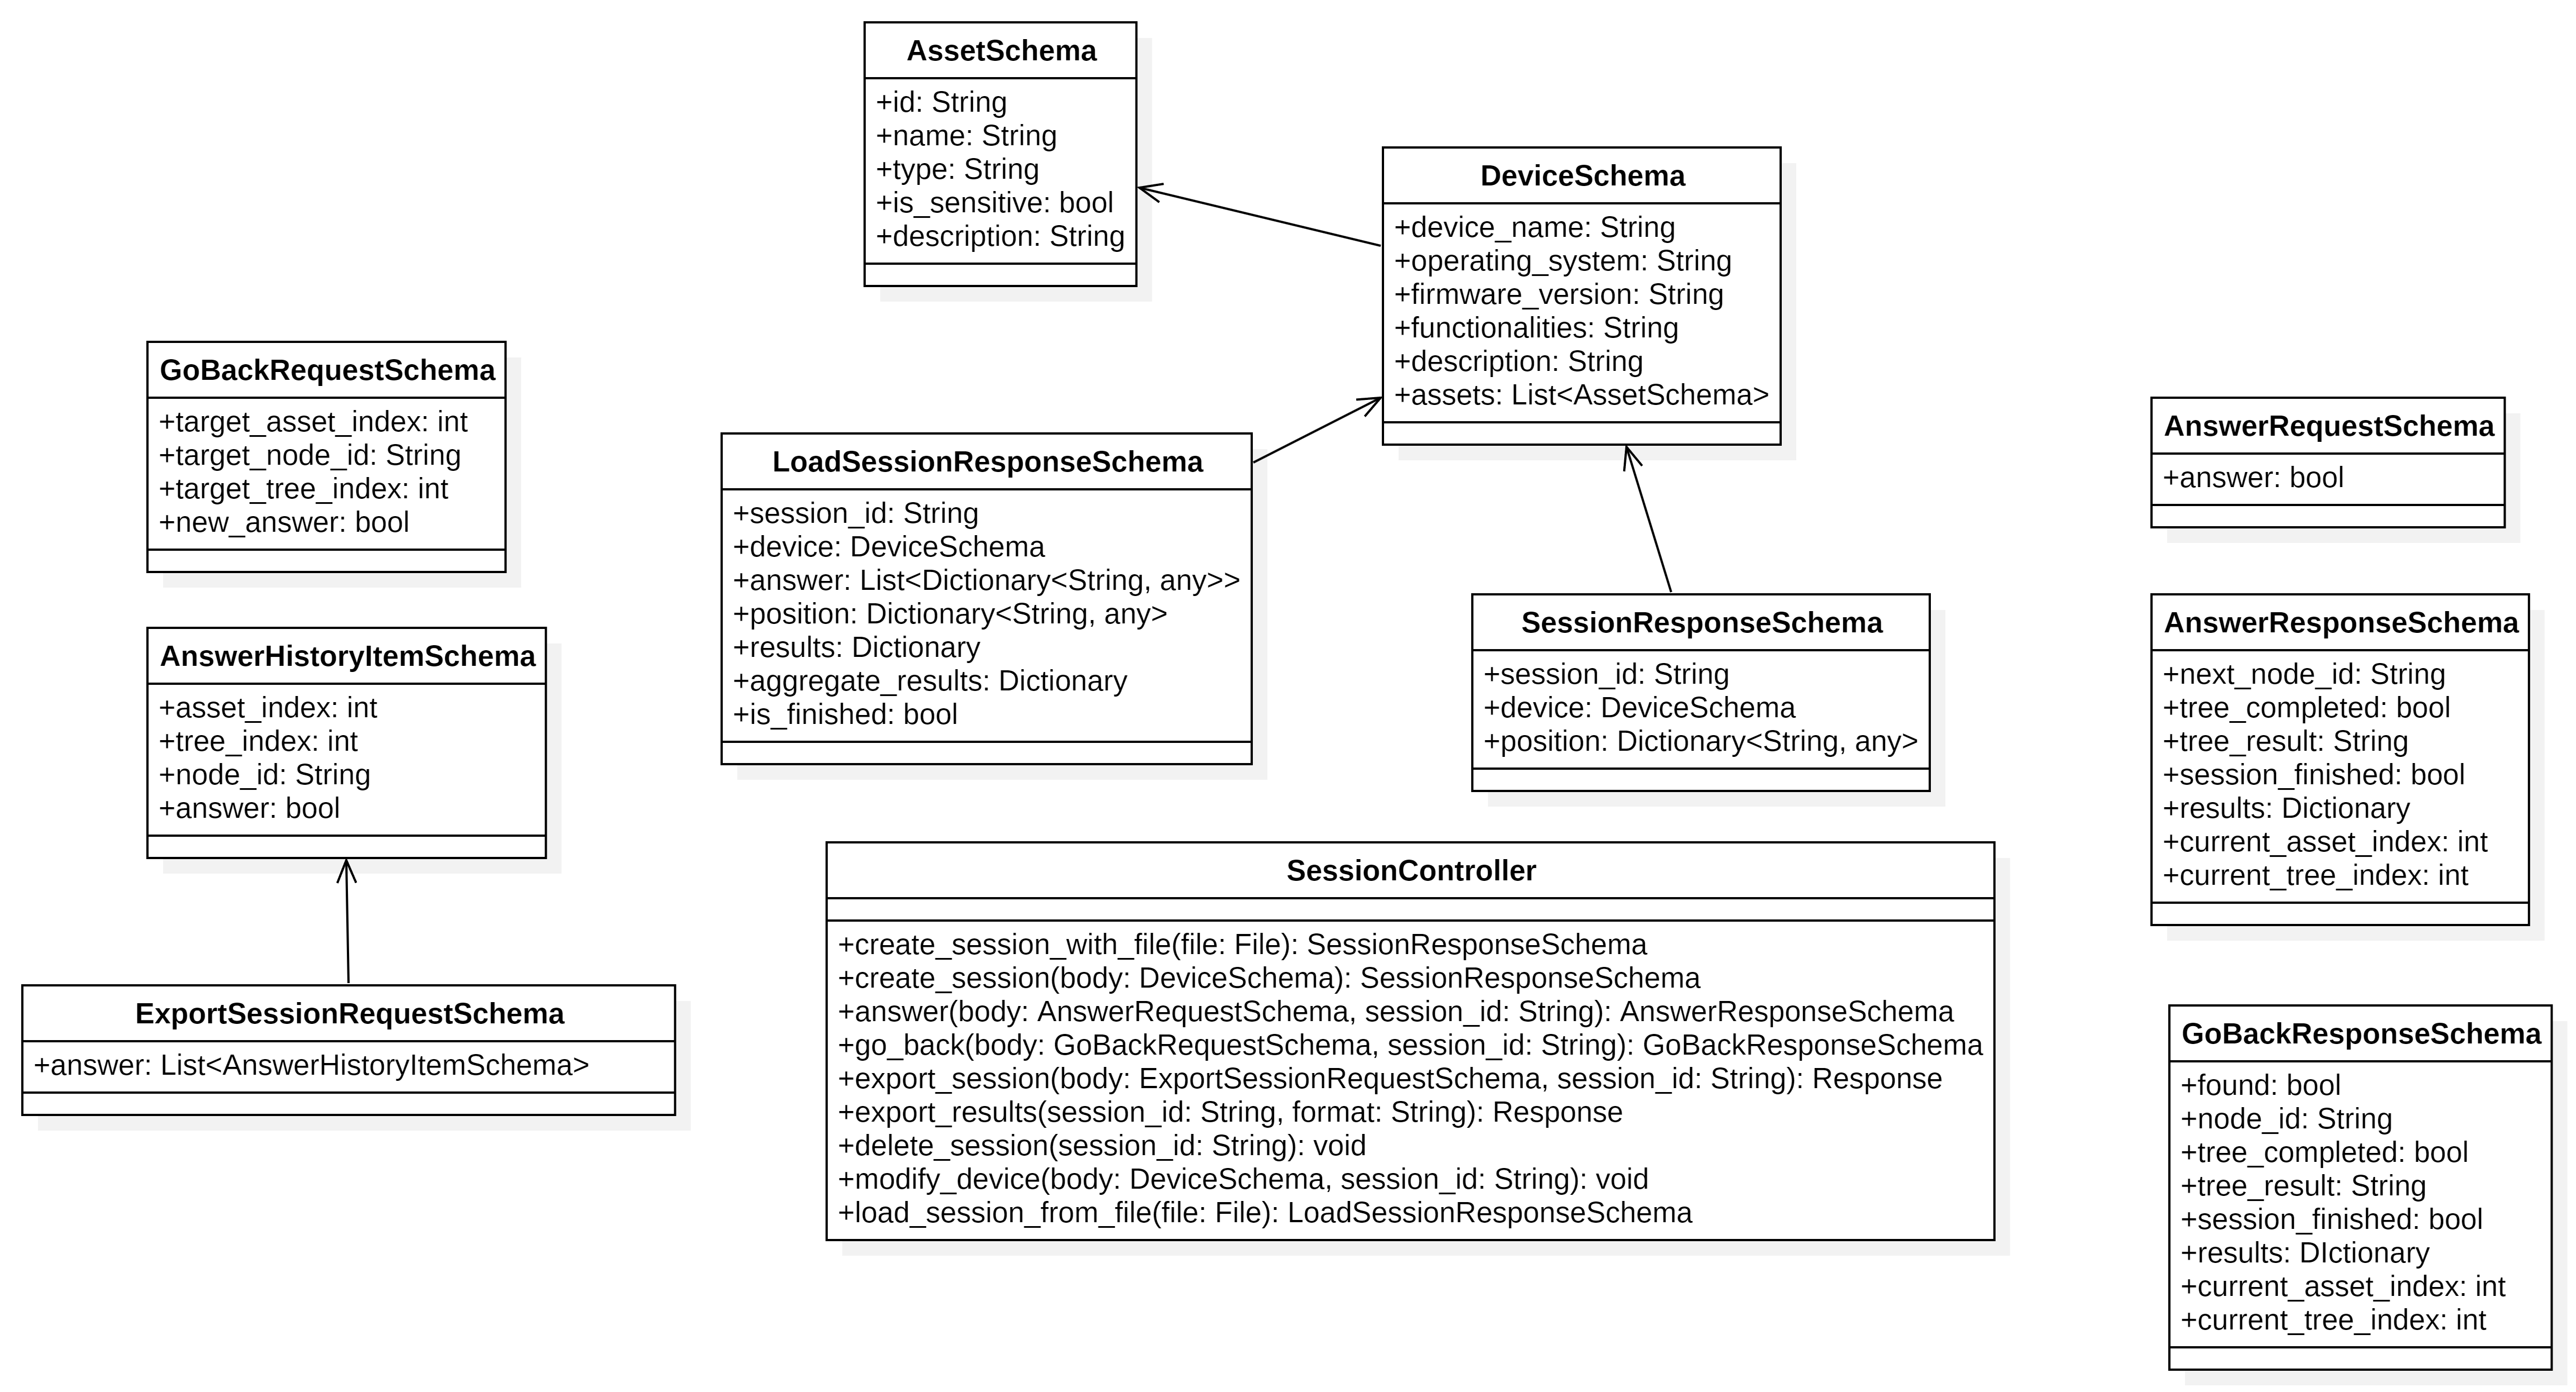
\includegraphics[width=1\linewidth]{../../../Assets/Classi/SessionController.png}
                              \caption{SessionController: Classe e Schema di validazione}
                        \end{figure}
                    \end{center}

                    Gli \textit{endpoint}\textsubscript{\href{https://atlasteam9.github.io/Atlas/glossario.html\#Endpoint}{G}} gestiti dal \textbf{SessionController} sono i seguenti: 

                    \begin{itemize}
                        \item {\ttfamily create\_session\_with\_file(file: File(...)) : SessionResponseSchema} \\ Permette di avviare una nuova sessione di test caricando un file JSON contenente le specifiche del dispositivo. Restituisce i dati necessari utili per inizializzare la sessione, validati mediante il \textbf{SessionResponseSchema} ;
                        \item {\ttfamily create\_session(body: DeviceSchema): SessionResponseSchema} \\ Svolge la stessa funzione dell'\textit{endpoint}\textsubscript{\href{https://atlasteam9.github.io/Atlas/glossario.html\#Endpoint}{G}} precedente, ma riceve i dati del dispositivo direttamente come oggetto JSON nel corpo della richiesta (body). È utile per integrazioni dirette senza passaggio da file system. I dati in ingresso vengono validati dal \textbf{DeviceSchema} e quelli in uscita dal \textbf{SessionResponseSchema} ;                         
                        \item {\ttfamily answer(body: AnswerRequestSchema, session\_id: String) : AnswerResponseSchema} \\ Registra la risposta (Sì/No) al \textit{nodo}\textsubscript{\href{https://atlasteam9.github.io/Atlas/glossario.html\#Nodo}{G}} corrente dell'albero decisionale attivo. Restituisce le informazioni sul \textit{nodo}\textsubscript{\href{https://atlasteam9.github.io/Atlas/glossario.html\#Nodo}{G}} successivo o l'eventuale completamento dell'albero o dell'intera sessione. I dati in ingresso vengono validati dal \textbf{AnswerRequestSchema} e quelli in uscita dal \textbf{AnswerResponseSchema} ; 
                        \item {\ttfamily go\_back(body: GoBackRequestSchema, session\_id: String): GoBackResponseSchema} \\ Consente all'utente di tornare a un \textit{nodo}\textsubscript{\href{https://atlasteam9.github.io/Atlas/glossario.html\#Nodo}{G}} specifico della cronologia all'interno dell'asset, permettendo di modificare una risposta precedente. Ricalcola automaticamente il percorso e la posizione corrente nel test. I dati in ingresso vengono validati dal \textbf{GoBackRequestSchema} e quelli in uscita dal \textbf{GoBackResponseSchema} ; 
                        \item {\ttfamily export\_session(body: ExportSessionRequestSchema, session\_id: String): Response} \\ Genera e restituisce un file JSON scaricabile che contiene lo stato completo della sessione (dati dispositivo, risposte e progressi). Serve per il backup o per riprendere il test in un secondo momento ; 
                        \item {\ttfamily export\_results(session\_id: String, format: String = "\textit{csv}\textsubscript{\href{https://atlasteam9.github.io/Atlas/glossario.html\#CSV}{G}}"): Response} \\ Elabora i risultati aggregati della conformità e li restituisce in formato \textit{CSV}\textsubscript{\href{https://atlasteam9.github.io/Atlas/glossario.html\#CSV}{G}} o PDF. È l'\textit{endpoint}\textsubscript{\href{https://atlasteam9.github.io/Atlas/glossario.html\#Endpoint}{G}} dedicato alla generazione della reportistica finale di conformità ; 
                        \item {\ttfamily delete\_session(session\_id: String): void} \\ Rimuove definitivamente la sessione dalla memoria volatile del \textit{server}\textsubscript{\href{https://atlasteam9.github.io/Atlas/glossario.html\#Server}{G}} e cancella il relativo file di persistenza dal disco. Restituisce uno stato di successo senza contenuto ;
                        \item {\ttfamily modify\_device(body: DeviceSchema, session\_id: String):  void} \\ Permette di aggiornare le informazioni descrittive o gli asset del dispositivo prima che il test abbia inizio. Ricrea la sessione mantenendo lo stesso ID per riflettere le modifiche apportate. I dati in ingresso vengono validati dal \textbf{DeviceSchema};
                        \item {\ttfamily load\_session\_from\_file(file: File(...)):  LoadSessionReponseSchema} \\ Carica una sessione precedentemente esportata da file JSON. Restituisce lo stato completo della sessione (device, posizione, risultati, risposte). I dati in uscita vengono validati dal \textbf{LoadSessionResponseSchema}.
                    \end{itemize}

                    L'utilizzo della classe \textbf{Response} di FastAPI (o delle sue sottoclassi) è preferibile rispetto a uno schema Pydantic quando  serve la gestione dei File Binari e Media Type. 
                    
                \paragraph{TreesController}\mbox{}\\
                    Controller FastAPI che gestisce l'\textit{endpoint}\textsubscript{\href{https://atlasteam9.github.io/Atlas/glossario.html\#Endpoint}{G}} per ottenere i \textit{decision tree}\textsubscript{\href{https://atlasteam9.github.io/Atlas/glossario.html\#DecisionTree}{G}} dal backend.

                    \begin{center}
                        \begin{figure}[H]
                              \centering
                              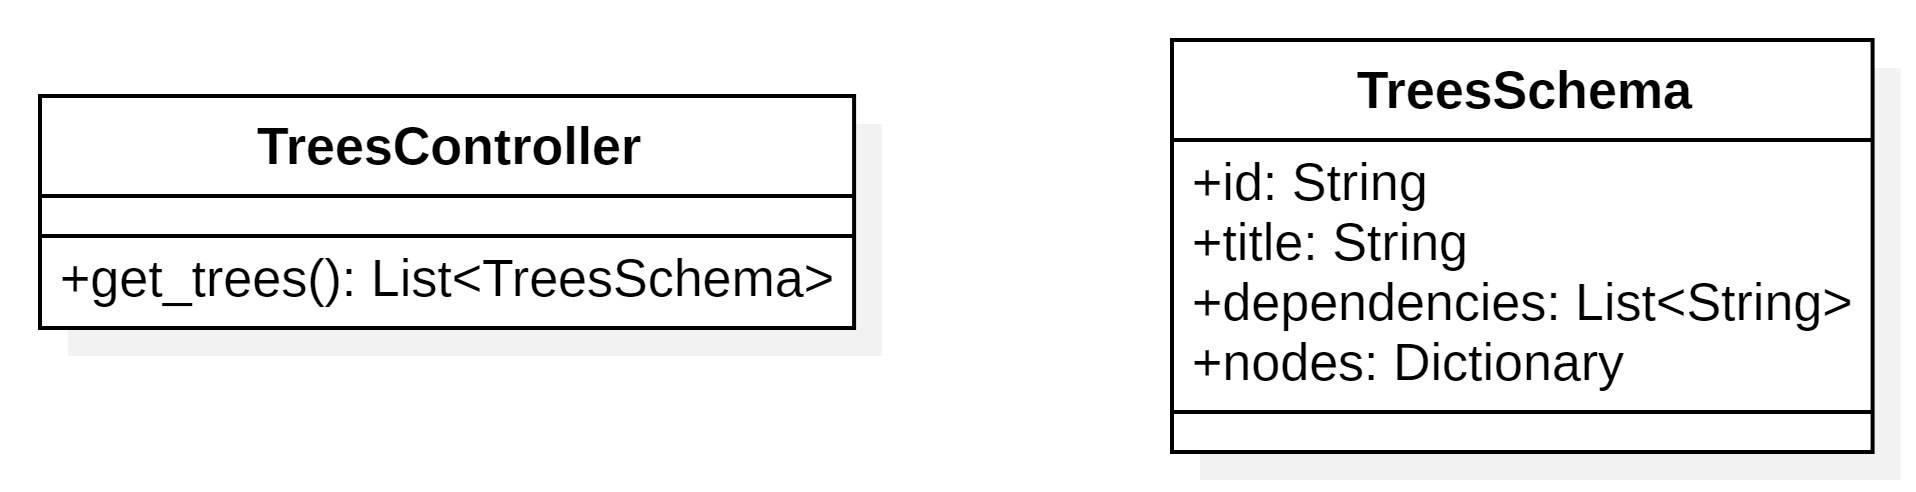
\includegraphics[width=1\linewidth]{../../../Assets/Classi/TreesController.png}
                              \caption{TreesController: Classe e Schema di validazione}
                        \end{figure}
                    \end{center}

                    \textbf{TreesController} gestisce un unico \textit{endpoint}\textsubscript{\href{https://atlasteam9.github.io/Atlas/glossario.html\#Endpoint}{G}}: 

                    \begin{itemize}
                        \item {\ttfamily get\_trees() : list<TreesSchema> } \\ Utilizzato all'avvio dell'applicazione, permette di avere gli alberi immediatamente pronti nel frontend. I dati in uscita vengono validati dal \textbf{TreesSchema}
                    \end{itemize}

            \subsubsection{Application Layer}
                \textbf{Scopo}: Orchestra i flussi di dati e implementa i casi d'uso (Use Cases) dell'applicazione.

                \noindent \textbf{Responsabilità}: Questo layer non contiene logica di business pura, ma coordina l'esecuzione delle operazioni chiamando i \textit{servizi}\textsubscript{\href{https://atlasteam9.github.io/Atlas/glossario.html\#Servizi}{G}} del dominio e le infrastrutture. Gestisce lo stato dell'applicazione (AppState) e definisce le interfacce per le operazioni come la creazione di sessioni o il recupero dei dati.\textbf{}
                \\
                \noindent Tutte le interfacce seguono lo stesso schema: unico metodo {\ttfamily execute()} tipizzato su un request e un response specifici. Inoltre tutti gli UseCase concreti del SessionController utilizzano l'\textit{interfaccia}\textsubscript{\href{https://atlasteam9.github.io/Atlas/glossario.html\#Interfaccia}{G}} \textbf{ISessionService} che astrae metodi utili alla manipolazione della sessione.  
            
                \paragraph{AppState}\mbox{}\\
                    AppState è una semplice classe che funge da gestore dello stato globale in memoria per l'applicazione, definendo due attributi principali: una \textit{lista}\textsubscript{\href{https://atlasteam9.github.io/Atlas/glossario.html\#Lista}{G}} di oggetti DecisionTree (trees) e un dizionario che associa identificatori testuali a oggetti Session (sessions). Viene utilizzata per mantenere in cache i dati essenziali per l'intera durata del ciclo di vita dell'applicazione FastAPI. All'avvio del \textit{server}\textsubscript{\href{https://atlasteam9.github.io/Atlas/glossario.html\#Server}{G}}  (tramite il \textbf{gestore di contesto lifespan}), AppState.trees viene inizializzato e popolato caricando in memoria tutti gli alberi decisionali dal file system tramite la classe FileTreeProvider. In questo modo i dati restano rapidamente accessibili per le successive richieste \textit{API}\textsubscript{\href{https://atlasteam9.github.io/Atlas/glossario.html\#API}{G}}, per poi venire esplicitamente rimossi (AppState.trees = []) durante la fase di spegnimento e pulizia dell'applicazione.

            
                \paragraph{ICreateSessionUseCase}\mbox{}\\
                    Contratto per la creazione di una sessione a partire da un dizionario proveniente da un file json caricato.
                    
                    \begin{center}
                        \begin{figure}[H]
                              \centering
                              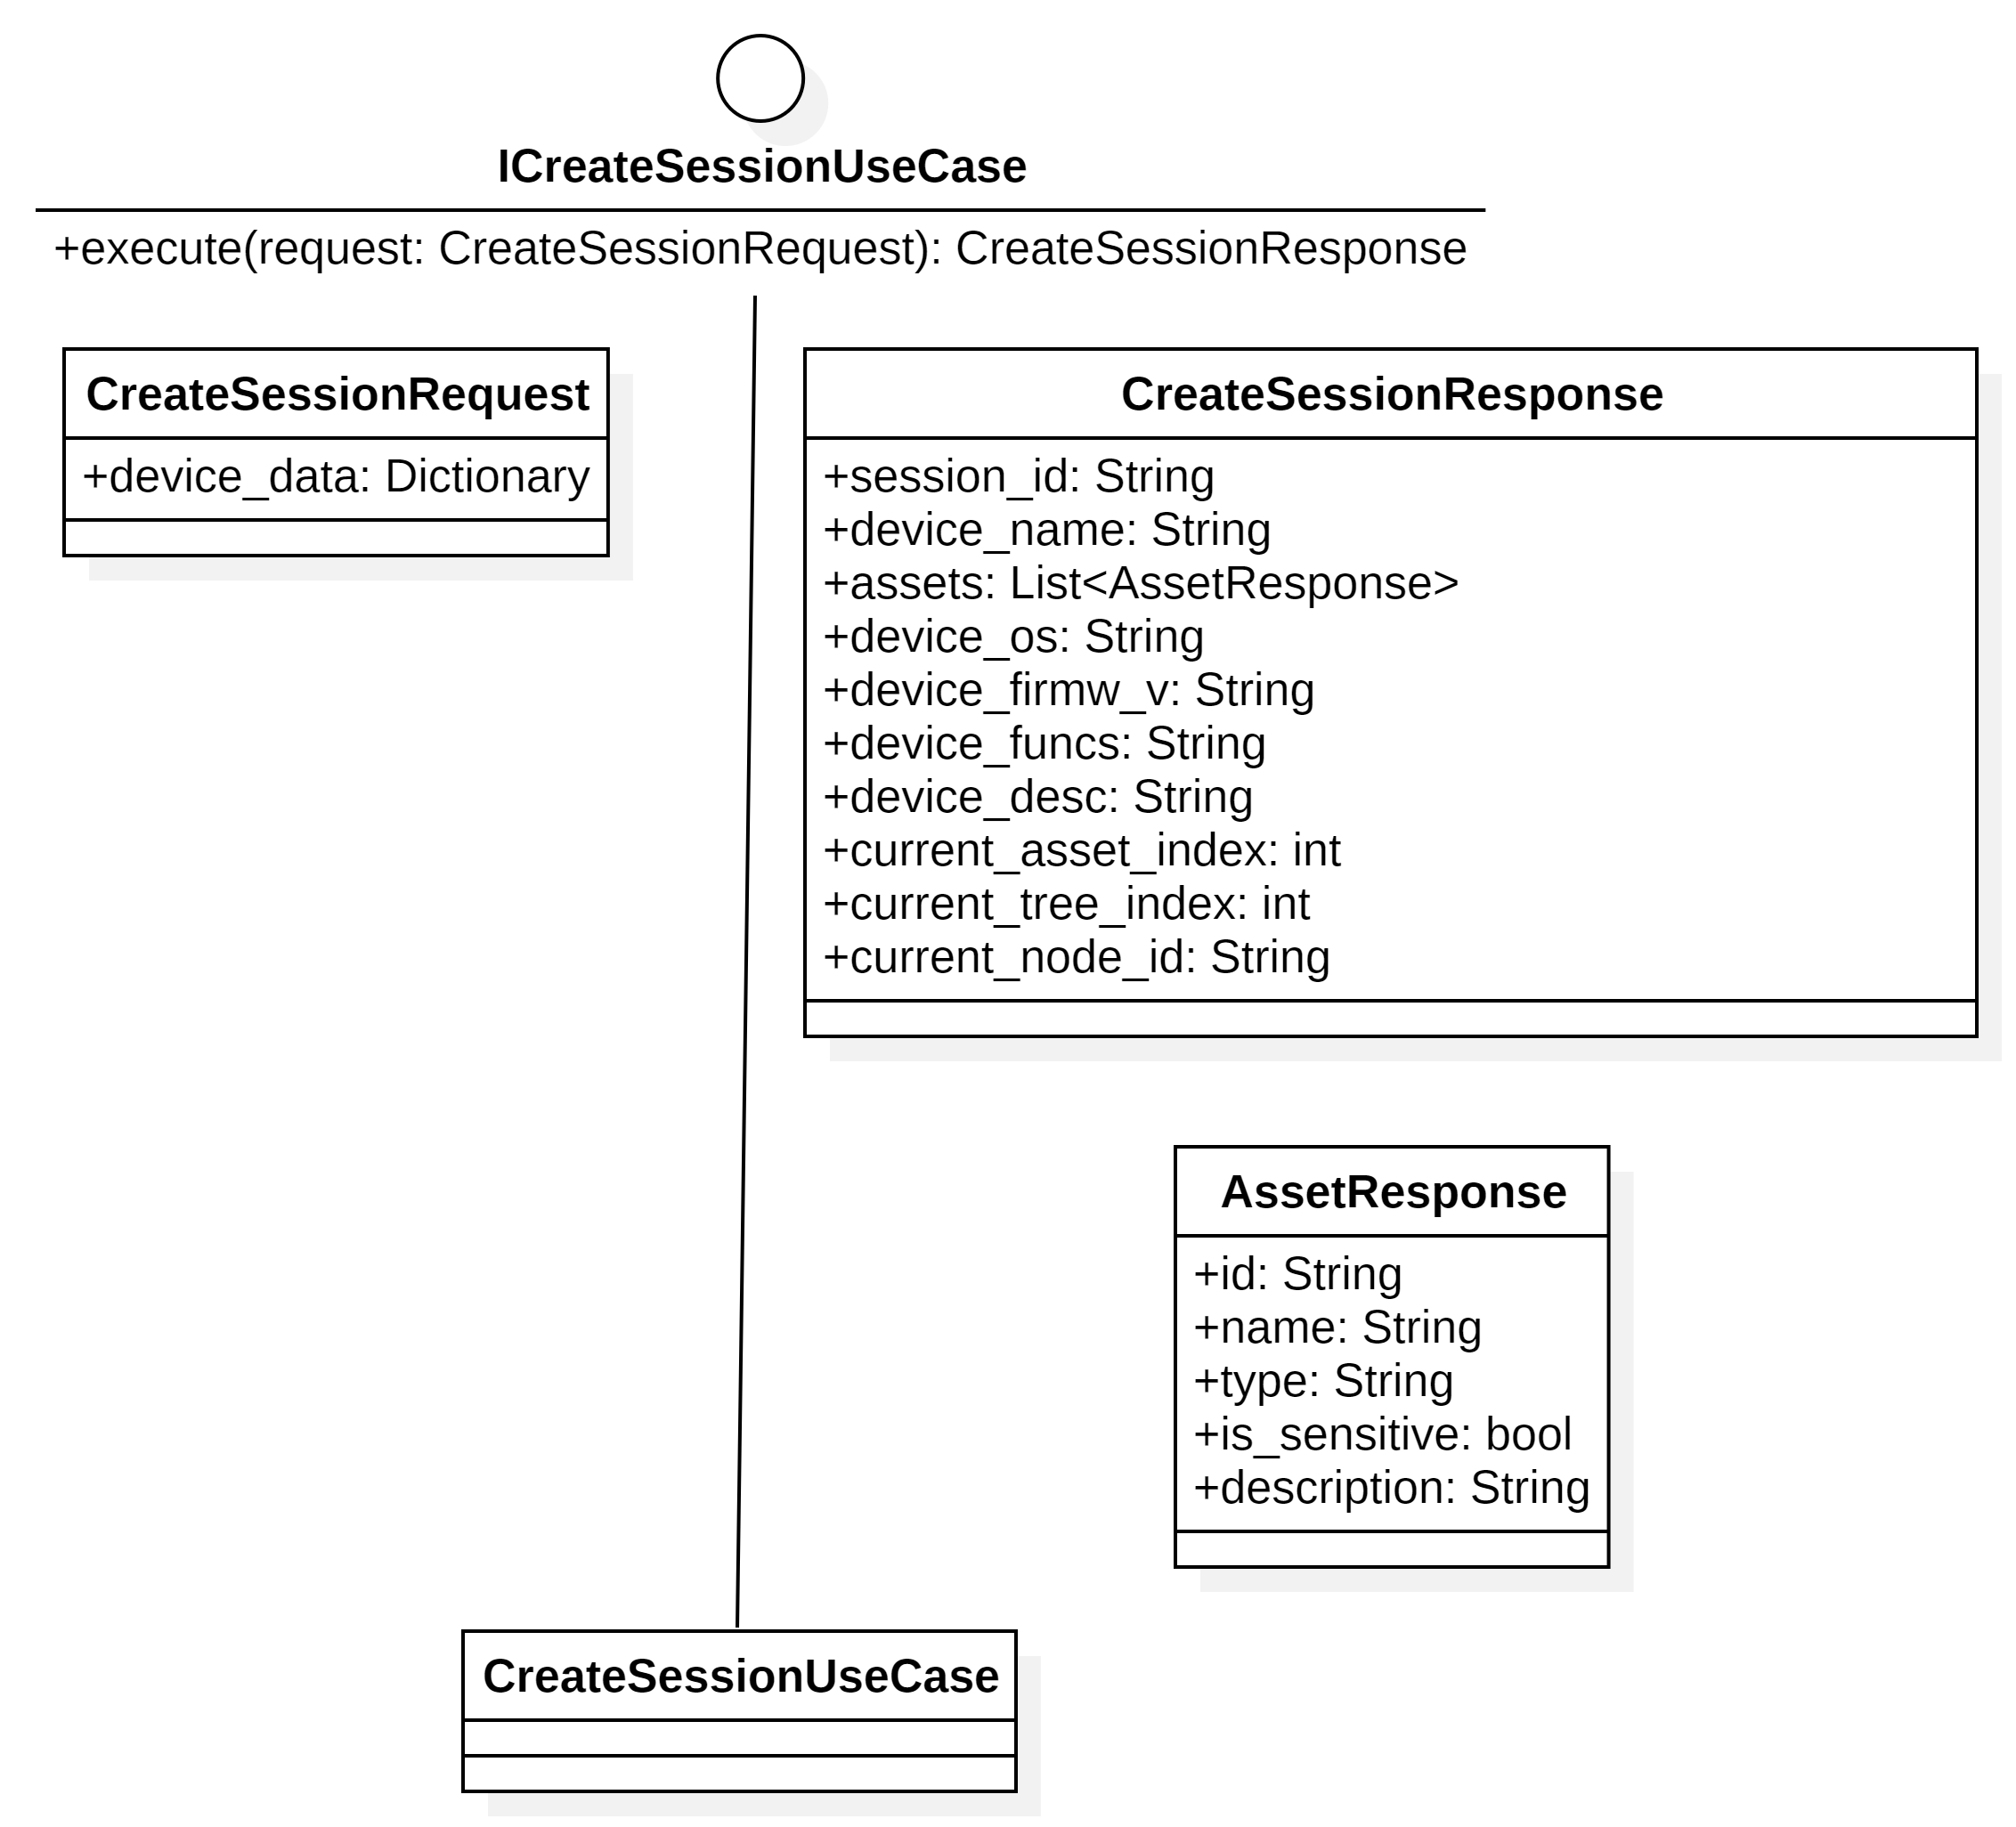
\includegraphics[width=.8\linewidth]{../../../Assets/Classi/CreateSessionUC.png}
                              \caption{CreateSessionUseCase: interfaccia, DTOs e classe}
                        \end{figure}
                    \end{center}
                    

                \paragraph{CreateSessionRequest}\mbox{}\\
                    DTO di richiesta per la creazione della sessione.\\\\
                    \textbf{Attributi}
                    \begin{itemize}
                        \item {\ttfamily device\_data: Dictionary}: dizionario contenente le informazioni del dispositivo.
                    \end{itemize}

                \paragraph{AssetResponse}\mbox{}\\
                    DTO di risposta contenente gli asset di un dispositivo.\\\\
                    \textbf{Attributi}
                    \begin{itemize}
                        \item {\ttfamily id: String}: id dell'asset;
                        \item {\ttfamily name: String}: nome dell'asset;
                        \item {\ttfamily type: String}: tipo dell'asset;
                        \item {\ttfamily is\_sensitive: bool}: flag di sensibilità dell'asset;
                        \item {\ttfamily description: String}: descrizione dell'asset.
                    \end{itemize}

                \paragraph{CreateSessionResponse}\mbox{}\\
                    DTO di risposta alla creazione della sessione.\\\\
                    \textbf{Attributi}
                    \begin{itemize}
                        \item {\ttfamily session\_id: String}: id univoco della sessione;
                        \item {\ttfamily device\_name: String}: nome del dispositivo oggetto di verifica;
                        \item {\ttfamily assets: list<AssetResponse>}: \textit{lista}\textsubscript{\href{https://atlasteam9.github.io/Atlas/glossario.html\#Lista}{G}} degli asset del dispositivo;
                        \item {\ttfamily device\_os: String}, {\ttfamily device\_firmw\_v: String}, {\ttfamily device\_funcs: String}, {\ttfamily device\_desc: String}: metadati relativi al dispositivo;
                        \item {\ttfamily current\_asset\_index: int}: indice dell'asset corrente;
                        \item {\ttfamily current\_tree\_index: int}: indice dell'albero corrente;
                        \item {\ttfamily current\_node\_id: String}: id del \textit{nodo}\textsubscript{\href{https://atlasteam9.github.io/Atlas/glossario.html\#Nodo}{G}} corrente.
                    \end{itemize}


                \paragraph{CreateSessionUseCase}\mbox{}\\
                    Valida il dizionario del device tramite Pydantic, costruisce l'oggetto Device con i suoi asset e delega al SessionService la creazione della sessione.\\\\
                    \textbf{Attributo}
                    \begin{itemize}
                        \item {\ttfamily \_session\_service: ISessionService}
                    \end{itemize}
                    \textbf{Metodo}
                    \begin{itemize}
                        \item {\ttfamily execute(request: CreateSessionRequest): CreateSessionResponse}
                    \end{itemize}


                \paragraph{IAnswerUseCase}\mbox{}\\
                    Contratto per la risposta al \textit{nodo}\textsubscript{\href{https://atlasteam9.github.io/Atlas/glossario.html\#Nodo}{G}} corrente di una sessione.

                    \begin{center}
                        \begin{figure}[H]
                              \centering
                              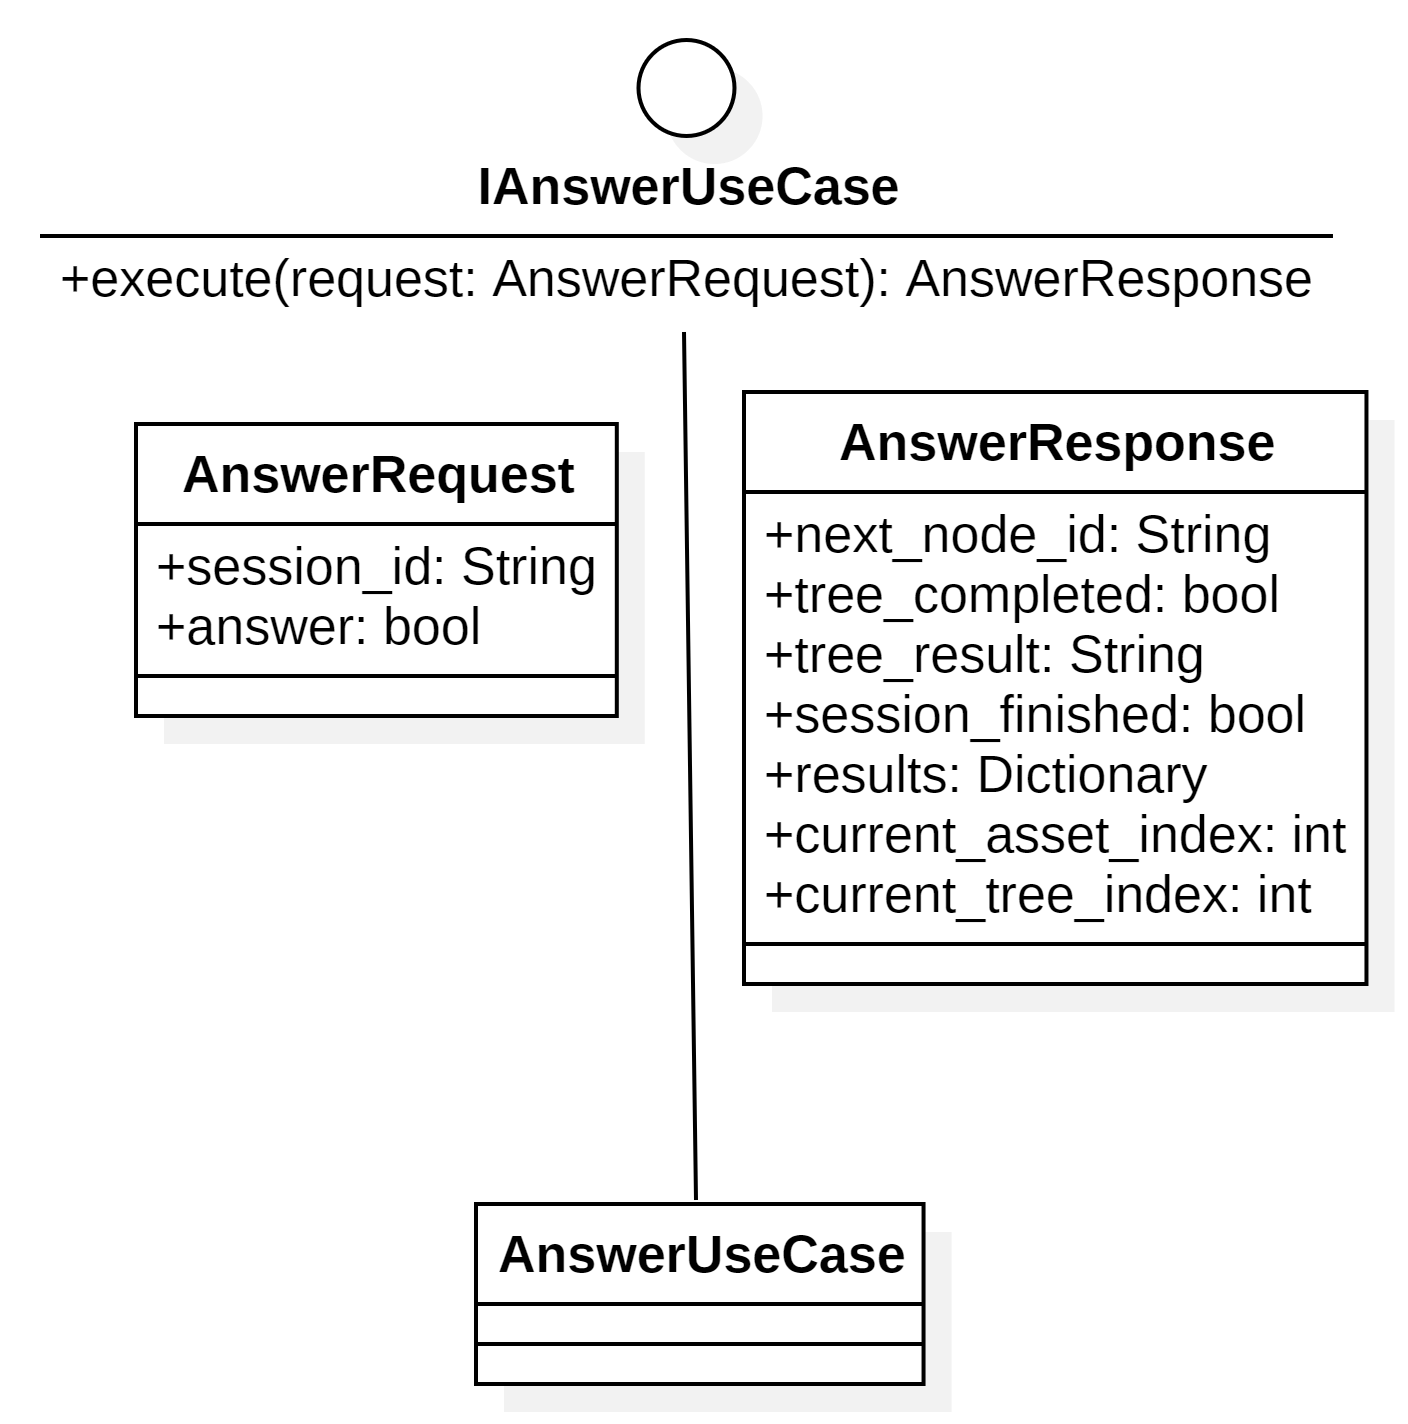
\includegraphics[width=.5\linewidth]{../../../Assets/Classi/AnswerUC.png}
                              \caption{AnswerUseCase: interfaccia, DTOs e classe}
                        \end{figure}
                    \end{center}
                    

                \paragraph{AnswerRequest}\mbox{}\\
                    DTO di richiesta di invio della risposta al \textit{nodo}\textsubscript{\href{https://atlasteam9.github.io/Atlas/glossario.html\#Nodo}{G}} corrente.\\\\
                    \textbf{Attributi}
                    \begin{itemize}
                        \item {\ttfamily session\_id: String}: id univoco della sessione;
                        \item {\ttfamily answer: bool}: risposta alla domanda del decision tree.
                    \end{itemize}

                \paragraph{AnswerResponse}\mbox{}\\
                    DTO di risposta al completamento del \textit{nodo}\textsubscript{\href{https://atlasteam9.github.io/Atlas/glossario.html\#Nodo}{G}} corrente.\\\\
                    \textbf{Attributi}
                    \begin{itemize}
                        \item {\ttfamily next\_node\_id: String}: id del prossimo \textit{nodo}\textsubscript{\href{https://atlasteam9.github.io/Atlas/glossario.html\#Nodo}{G}} con la prossima domanda da rispondere;
                        \item {\ttfamily tree\_completed: bool}: flag di completamento dell'albero;
                        \item {\ttfamily tree\_result String}: risultato di completamento dell'albero;
                        \item {\ttfamily session\_finished: bool}: flag di completamento della sessione;
                        \item {\ttfamily results: Dictionary}; dizionario contenente i risultati della sessione;
                        \item {\ttfamily current\_asset\_index: int}; indice dell'asset corrente;
                        \item {\ttfamily current\_tree\_index: int}; indice dell'albero corrente;
                    \end{itemize}

                \paragraph{AnswerUseCase}\mbox{}\\
                    Carica la sessione tramite il service, chiama {\ttfamily session.answer()} e salva lo stato aggiornato. Restituisce {\ttfamily AnswerResponse} con il prossimo \textit{nodo}\textsubscript{\href{https://atlasteam9.github.io/Atlas/glossario.html\#Nodo}{G}}, il risultato dell'albero se completato e il flag di fine sessione.\\\\
                    \textbf{Attributo}
                    \begin{itemize}
                        \item {\ttfamily \_session\_service: ISessionService}
                    \end{itemize}
                    \textbf{Metodo}
                    \begin{itemize}
                        \item {\ttfamily execute(request: AnswerRequest): AnswerResponse}
                    \end{itemize}


                \paragraph{IGoBackUseCase}\mbox{}\\
                    Contratto per il ritorno a un \textit{nodo}\textsubscript{\href{https://atlasteam9.github.io/Atlas/glossario.html\#Nodo}{G}} precedente nella history del tree corrente.
                    
                    \begin{center}
                        \begin{figure}[H]
                              \centering
                              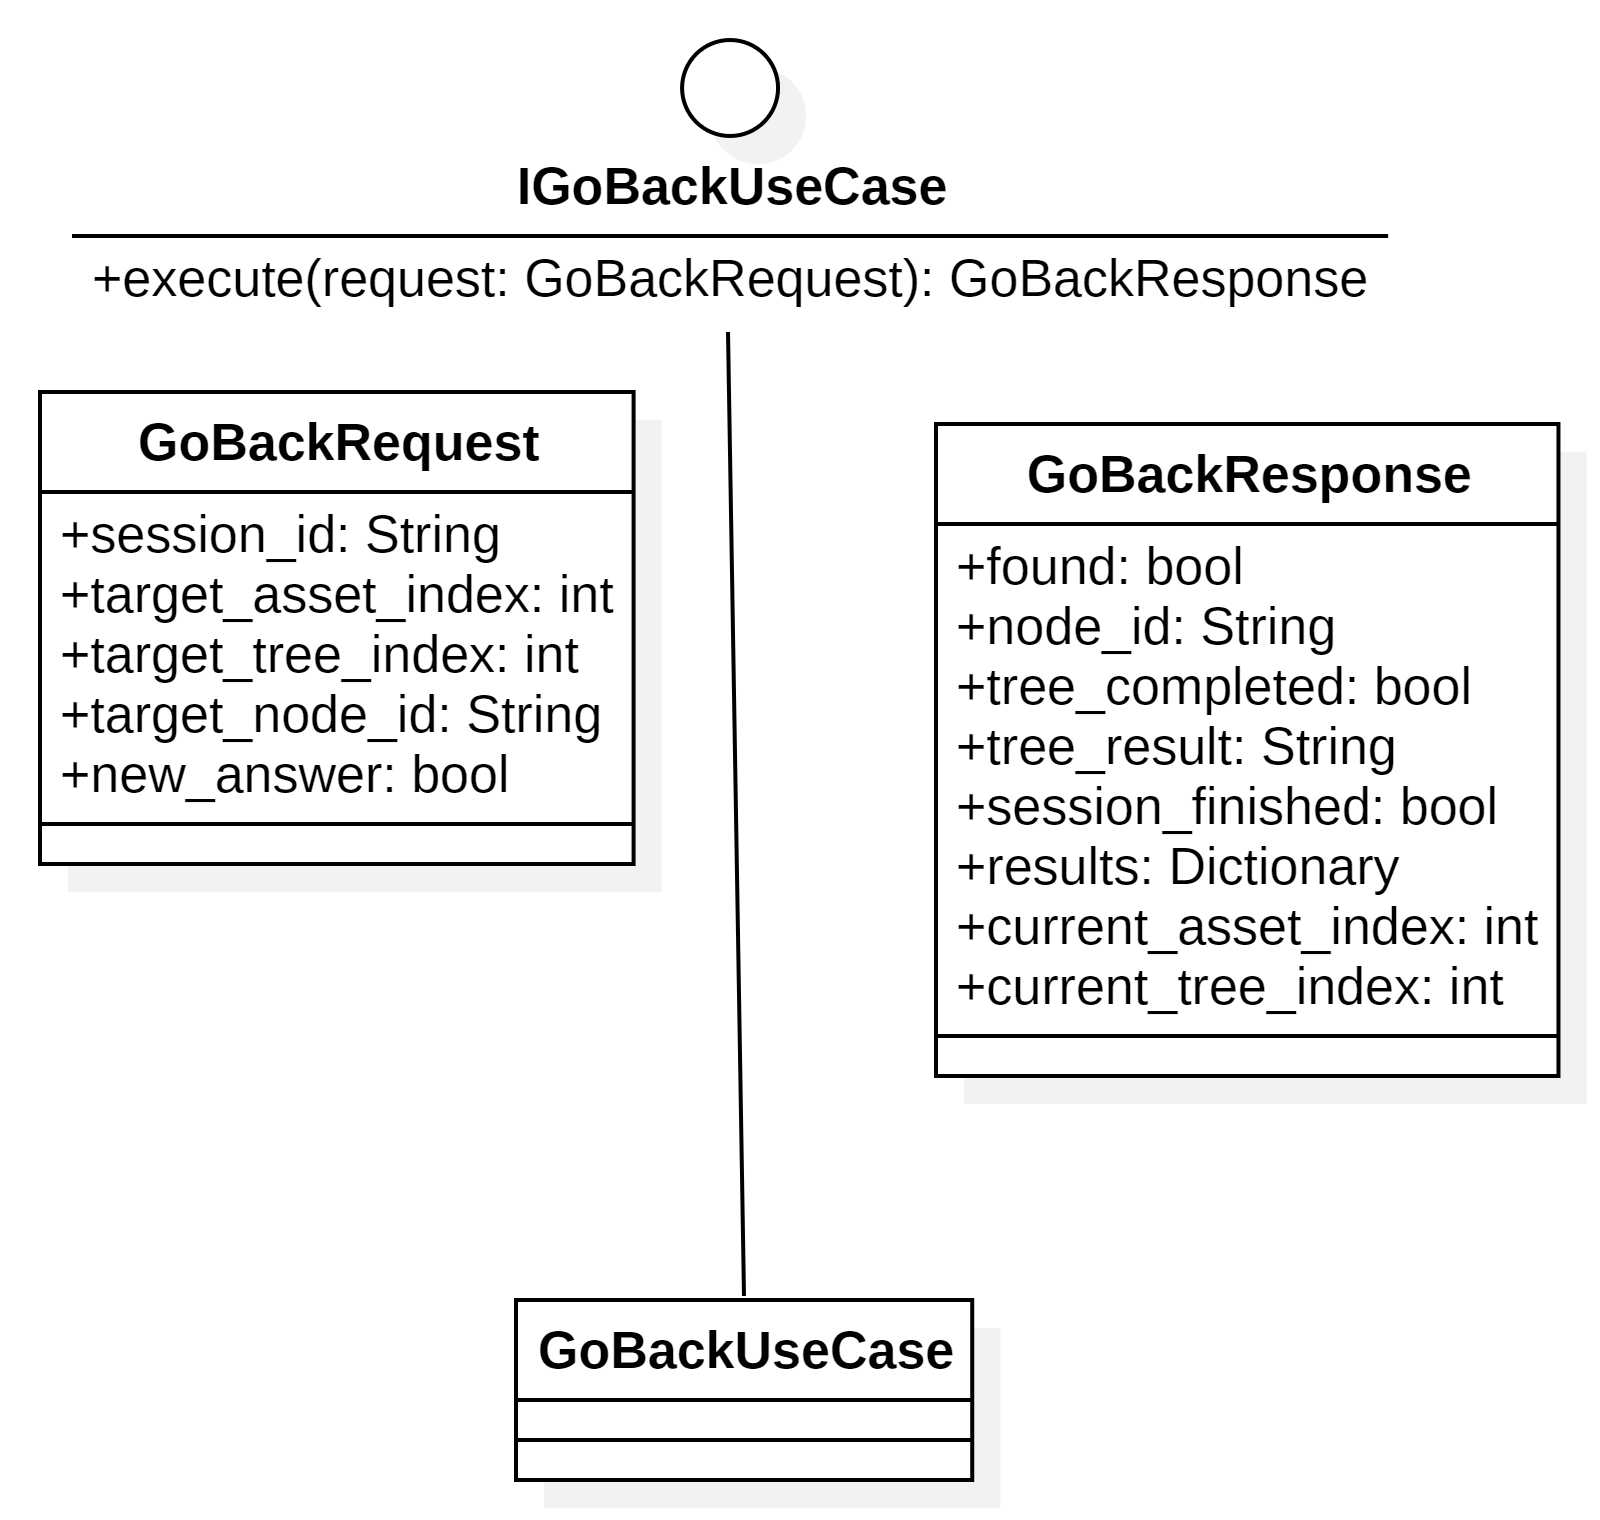
\includegraphics[width=.6\linewidth]{../../../Assets/Classi/GoBackUC.png}
                              \caption{GoBackUseCase: interfaccia, DTOs e classe}
                        \end{figure}
                    \end{center}
                    

                \paragraph{GoBackRequest}\mbox{}\\
                    DTO di richiesta per ritornare a un \textit{nodo}\textsubscript{\href{https://atlasteam9.github.io/Atlas/glossario.html\#Nodo}{G}} già risposto nell'albero corrente.\\\\
                    \textbf{Attributi}
                    \begin{itemize}
                        \item {\ttfamily session\_id: String}: id univoco della sessione;
                        \item {\ttfamily target\_asset\_index: int}: asset in cui si vuole cambiare la risposta;
                        \item {\ttfamily target\_tree\_index: String}: albero in cui si vuole cambiare la risposta;
                        \item {\ttfamily target\_node\_id: String}: \textit{nodo}\textsubscript{\href{https://atlasteam9.github.io/Atlas/glossario.html\#Nodo}{G}} in cui si vuole cambiare la risposta;
                        \item {\ttfamily new\_answer: bool}: nuova risposta data alla domanda;
                    \end{itemize}

                \paragraph{GoBackResponse}\mbox{}\\
                    DTO di risposta al ritorno indietro di un \textit{nodo}\textsubscript{\href{https://atlasteam9.github.io/Atlas/glossario.html\#Nodo}{G}} a cui l'utente aveva già risposto.\\\\
                    \textbf{Attributi}
                    \begin{itemize}
                        \item {\ttfamily found : bool}: flag di ritrovamento del \textit{nodo}\textsubscript{\href{https://atlasteam9.github.io/Atlas/glossario.html\#Nodo}{G}};
                        \item {\ttfamily node\_id : String}: id del \textit{nodo}\textsubscript{\href{https://atlasteam9.github.io/Atlas/glossario.html\#Nodo}{G}} (se ritrovato);
                        \item {\ttfamily tree\_completed: bool}: flag di completamento dell'albero;
                        \item {\ttfamily tree\_result: String}: risultato del completamento dell'albero;
                        \item {\ttfamily session\_finished: bool}: flag di completamento della sessione; 
                        \item {\ttfamily results: Dictionary}: dizionario contenente i risultati dei \textit{decision tree}\textsubscript{\href{https://atlasteam9.github.io/Atlas/glossario.html\#DecisionTree}{G}};
                        \item {\ttfamily current\_asset\_index: int}: indice dell'asset corrente;
                        \item {\ttfamily current\_tree\_index: int}: indice dell'albero corrente.
                    \end{itemize}

                \paragraph{GoBackUseCase}\mbox{}\\
                    Carica la sessione tramite il service, cerca il \textit{nodo}\textsubscript{\href{https://atlasteam9.github.io/Atlas/glossario.html\#Nodo}{G}} target nella navigation stack tramite l'id e chiama {\ttfamily session.go\_back()}.\\\\
                    \textbf{Attributo}
                    \begin{itemize}
                        \item {\ttfamily \_session\_service: ISessionService}
                    \end{itemize}
                    \textbf{Metodo}
                    \begin{itemize}
                        \item {\ttfamily execute(request: GoBackRequest): GoBackResponse}
                    \end{itemize}


                \paragraph{IExportResultsUseCase}\mbox{}\\
                    Contratto per l'\textit{esportazione}\textsubscript{\href{https://atlasteam9.github.io/Atlas/glossario.html\#Esportazione}{G}} dei risultati in un file esterno.
                    
                    \begin{center}
                        \begin{figure}[H]
                              \centering
                              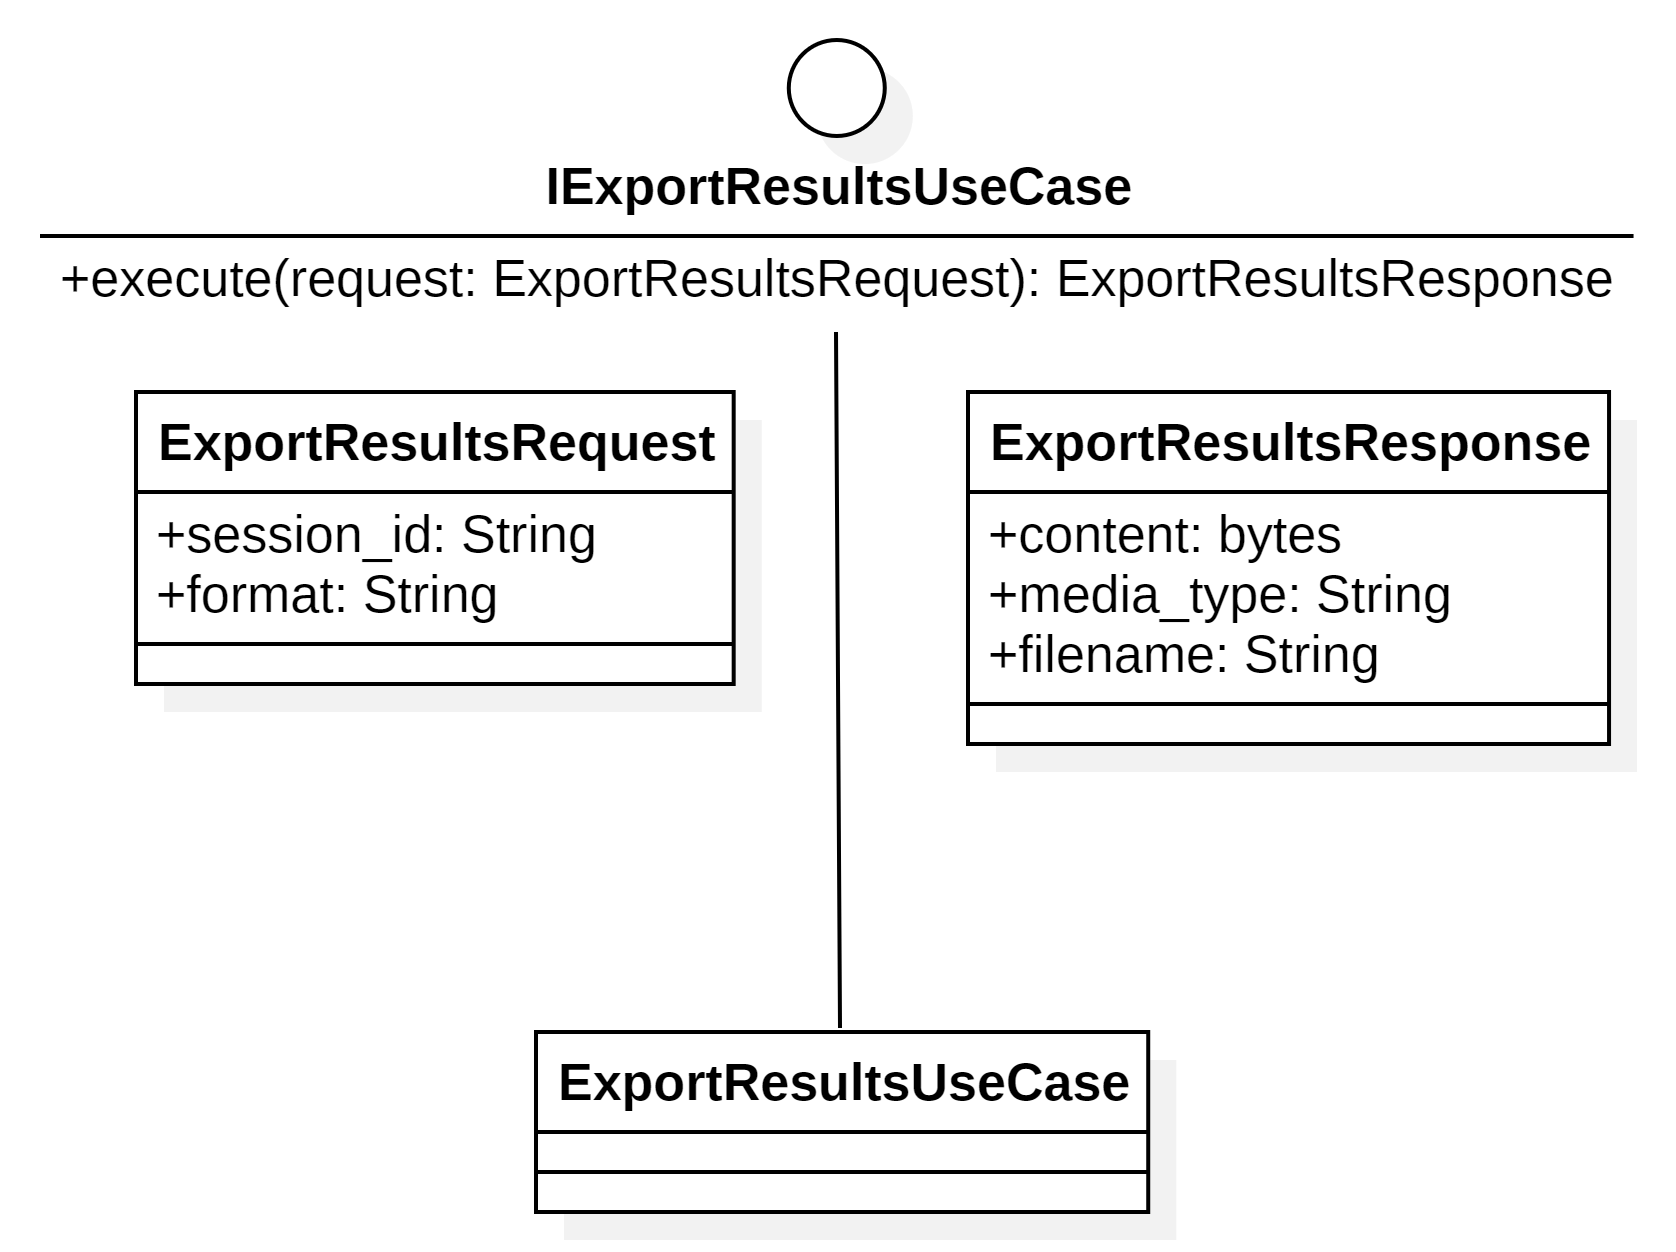
\includegraphics[width=.6\linewidth]{../../../Assets/Classi/ExportResultsUC.png}
                              \caption{ExportResultsUseCase: interfaccia, DTOs e classe}
                        \end{figure}
                    \end{center}

                \paragraph{ExportResultsRequest}\mbox{}\\
                    DTO di richiesta di \textit{esportazione}\textsubscript{\href{https://atlasteam9.github.io/Atlas/glossario.html\#Esportazione}{G}} risultati su un file esterno.\\\\
                    \textbf{Attributi}
                    \begin{itemize}
                        \item {\ttfamily session\_id: String}: id univoco della sessione;
                        \item {\ttfamily format: String}: formato di \textit{esportazione}\textsubscript{\href{https://atlasteam9.github.io/Atlas/glossario.html\#Esportazione}{G}} (csv/pdf).
                    \end{itemize}

                \paragraph{ExportResultsResponse}\mbox{}\\
                    DTO di risposta all'\textit{esportazione}\textsubscript{\href{https://atlasteam9.github.io/Atlas/glossario.html\#Esportazione}{G}} dei risultati del test su file.\\\\
                    \textbf{Attributi}
                    \begin{itemize}
                        \item {\ttfamily content: bytes}: contenuto del file;
                        \item {\ttfamily media\_type: String}: tipo di file (csv/pdf);
                        \item {\ttfamily filename: String}: nome del file.
                    \end{itemize}

                \paragraph{ExportResultsUseCase}\mbox{}\\
                    Carica la sessione tramite il service, seleziona l'exporter appropriato dal dizionario, chiama {\ttfamily export()} e restituisce i byte con media type e nome del file.\\\\
                    \textbf{Attributo}
                    \begin{itemize}
                        \item {\ttfamily \_session\_service: ISessionService}
                    \end{itemize}
                    \textbf{Metodo}
                    \begin{itemize}
                        \item {\ttfamily execute(request: ExportResultsRequest): ExportResultsResponse}
                    \end{itemize}


                \paragraph{IExportSessionUseCase}\mbox{}\\
                    Contratto per l'\textit{esportazione}\textsubscript{\href{https://atlasteam9.github.io/Atlas/glossario.html\#Esportazione}{G}} dell'intera sessione come file json scaricabile.
                    
                    \begin{center}
                        \begin{figure}[H]
                              \centering
                              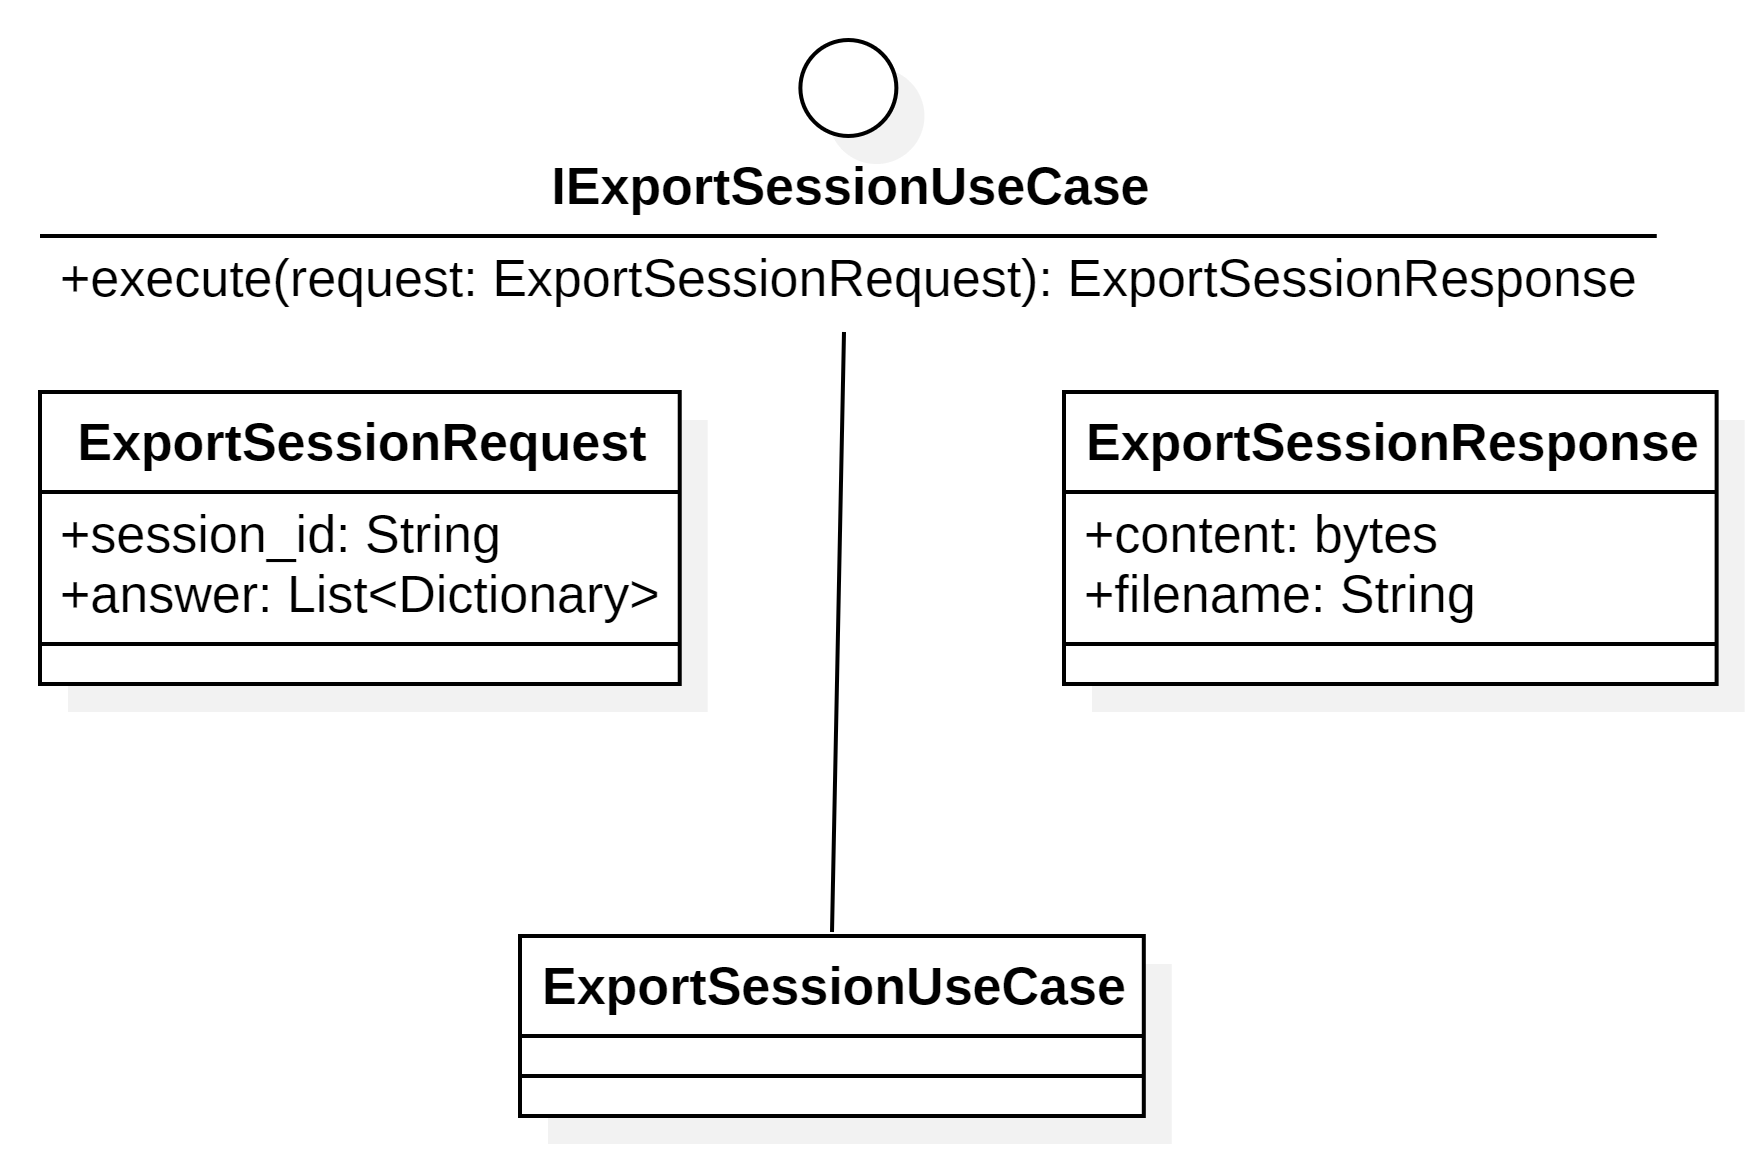
\includegraphics[width=.6\linewidth]{../../../Assets/Classi/ExportSessionUC.png}
                              \caption{ExportSessionUseCase: interfaccia, DTOs e classe}
                        \end{figure}
                    \end{center}
                    

                \paragraph{ExportSessionRequest}\mbox{}\\
                DTO di richiesta per l'\textit{esportazione}\textsubscript{\href{https://atlasteam9.github.io/Atlas/glossario.html\#Esportazione}{G}} della sessione su file.\\\\
                    \textbf{Attributi}
                    \begin{itemize}
                        \item {\ttfamily session\_id: String}: id univoco della sessione;
                        \item {\ttfamily answer: List<Dictionary>}: \textit{lista}\textsubscript{\href{https://atlasteam9.github.io/Atlas/glossario.html\#Lista}{G}} delle risposte date serializzate tramite dizionario.
                    \end{itemize}

                \paragraph{ExportSessionResponse}\mbox{}\\
                    DTO di risposta all'\textit{esportazione}\textsubscript{\href{https://atlasteam9.github.io/Atlas/glossario.html\#Esportazione}{G}} della sessione su file.\\\\
                    \textbf{Attributi}
                    \begin{itemize}
                        \item {\ttfamily content: bytes}: contenuto del file;
                        \item {\ttfamily filename: String}: nome del file.
                    \end{itemize}

                \paragraph{ExportSessionUseCase}\mbox{}\\
                    Carica la sessione tramite il service e serializza l'intero stato come json, restituendolo come bytes scaricabili.\\\\
                    \textbf{Attributo}
                    \begin{itemize}
                        \item {\ttfamily \_session\_service: ISessionService}
                    \end{itemize}
                    \textbf{Metodo}
                    \begin{itemize}
                        \item {\ttfamily execute(request: ExportSessionRequest): ExportSessionResponse}
                    \end{itemize}

                

                \paragraph{IDeleteSessionUseCase}\mbox{}\\
                    Contratto per la cancellazione di una sessione.
                    
                    \begin{center}
                        \begin{figure}[H]
                              \centering
                              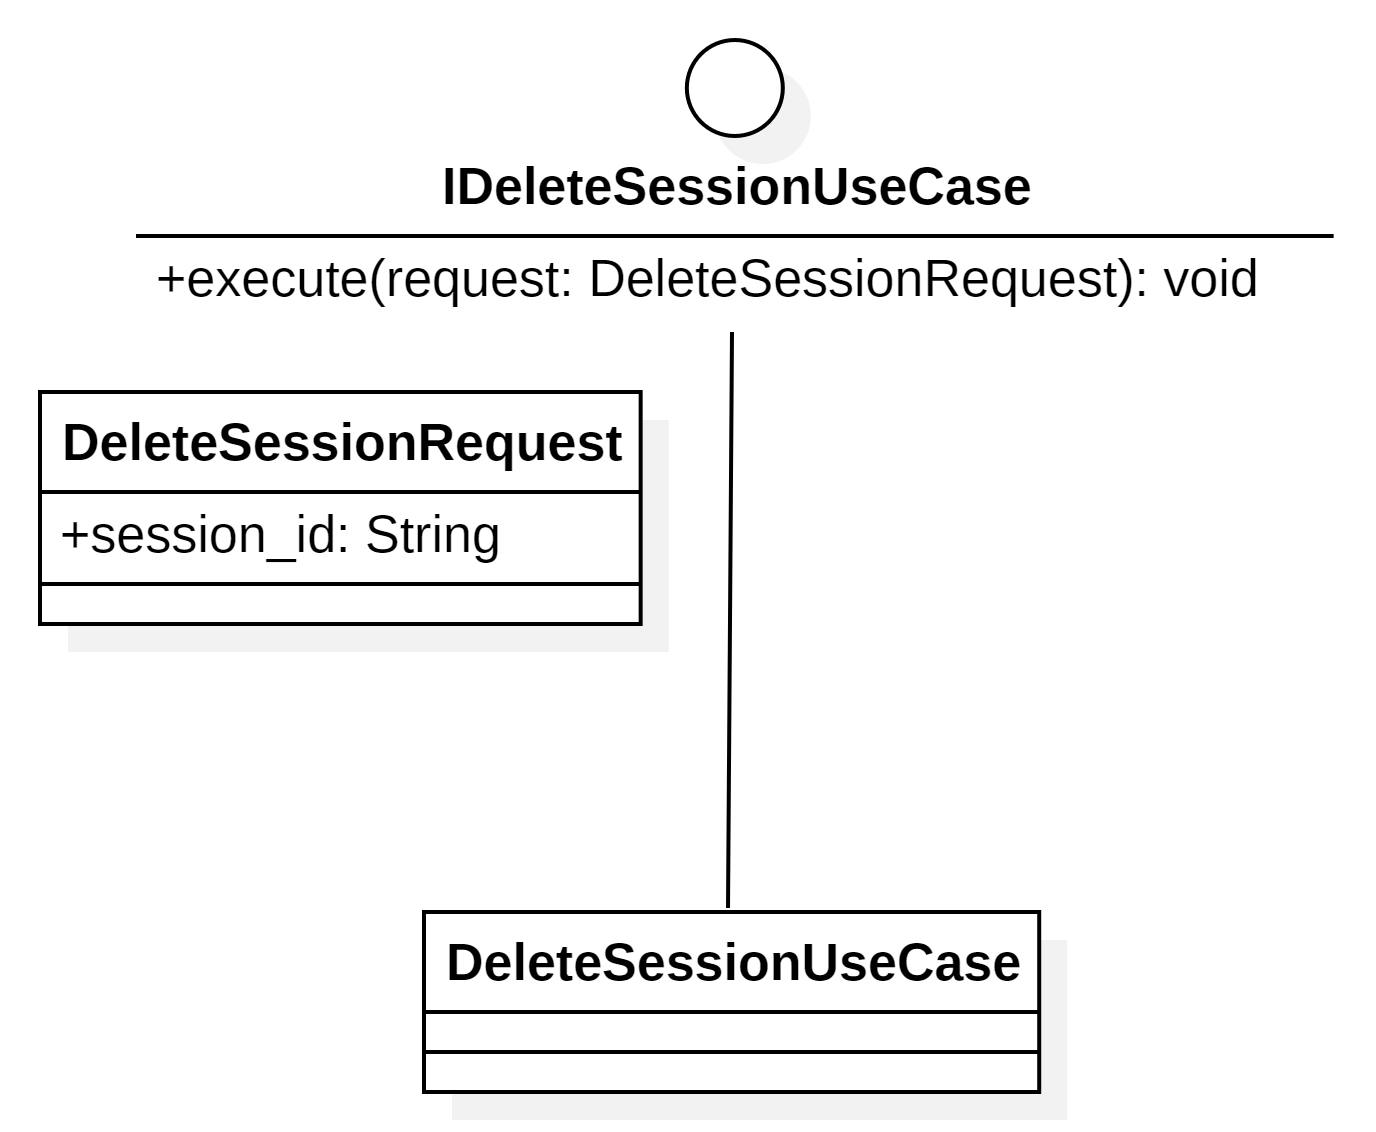
\includegraphics[width=.5\linewidth]{../../../Assets/Classi/DeleteSessionUC.png}
                              \caption{DeleteSessionUseCase: interfaccia, DTOs e classe}
                        \end{figure}
                    \end{center}


                \paragraph{DeleteSessionRequest}\mbox{}\\
                    DTO di richiesta per la cancellazione di una sessione. \\\\
                    \textbf{Attributi}
                    \begin{itemize}
                        \item {\ttfamily session\_id: String}: id univoco della sessione.
                    \end{itemize}

                \paragraph{DeleteSessionUseCase}\mbox{}\\
                    Verifica che la sessione esista e poi la elimina sia dalla cache che dal repository.\\\\
                    \textbf{Attributo}
                    \begin{itemize}
                        \item {\ttfamily \_session\_service: ISessionService}
                    \end{itemize}
                    \textbf{Metodo}
                    \begin{itemize}
                        \item {\ttfamily execute(request: DeleteSessionRequest): void}
                    \end{itemize}

                \paragraph{IModifyDeviceUseCase}\mbox{}\\
                    Contratto per la modifica del device creato manualmente. 
                    
                    \begin{center}
                        \begin{figure}[H]
                              \centering
                              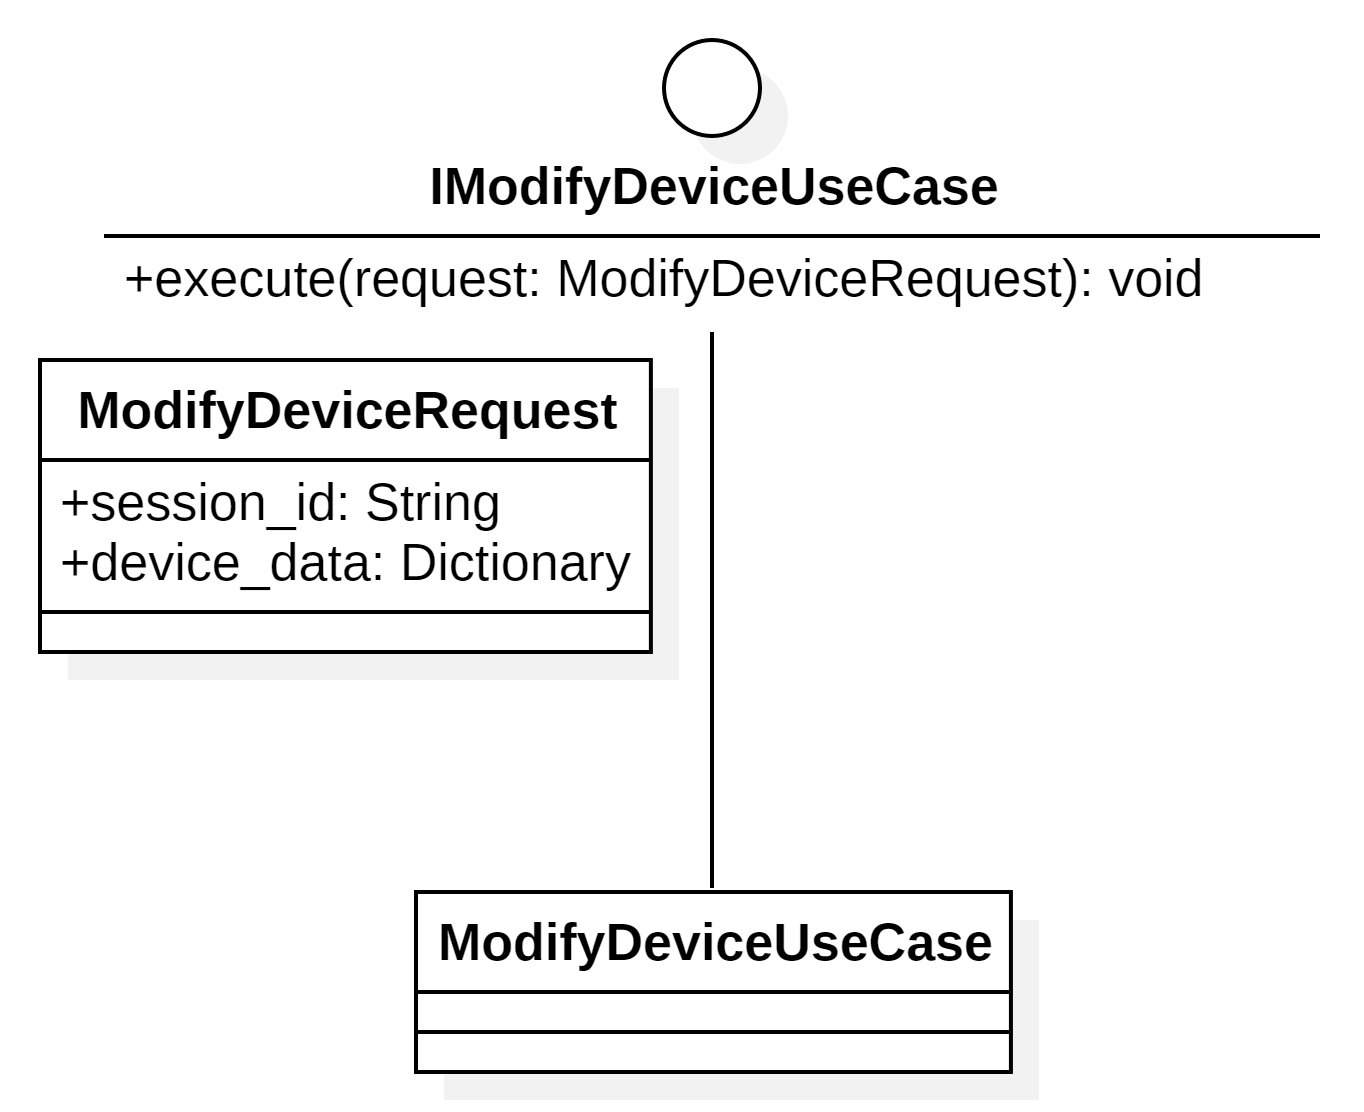
\includegraphics[width=.5\linewidth]{../../../Assets/Classi/ModifyDeviceUC.png}
                              \caption{ModifyDevice: interfaccia, DTOs e classe}
                        \end{figure}
                    \end{center}
                    

                \paragraph{ModifyDeviceRequest}\mbox{}\\
                    DTO di richiesta per modificare il device creato.\\\\
                    \textbf{Attributi}
                    \begin{itemize}
                        \item {\ttfamily session\_id: String}: id univoco della sessione in cui va modificato il device;
                        \item {\ttfamily device\_data: Dictionary}: dizionario con le nuove informazioni del device;
                    \end{itemize}

                \paragraph{ModifyDeviceUseCase}\mbox{}\\
                    Carica la sessione tramite il service, crea il nuovo device e sovrascrive la sessione precedente con la nuova modificata mediante la factory.\\\\
                    \textbf{Attributo}
                    \begin{itemize}
                        \item {\ttfamily \_session\_service: ISessionService}
                        \item {\ttfamily \_factory: SessionFactory}
                    \end{itemize}
                    \textbf{Metodo}
                    \begin{itemize}
                        \item {\ttfamily execute(request: ModifyDeviceRequest): void}
                    \end{itemize}

                \paragraph{ILoadSessionUseCase}\mbox{}\\
                    Contratto per l'upload di una sessione di test vecchia in formato JSON. 
                    
                    \begin{center}
                        \begin{figure}[H]
                              \centering
                              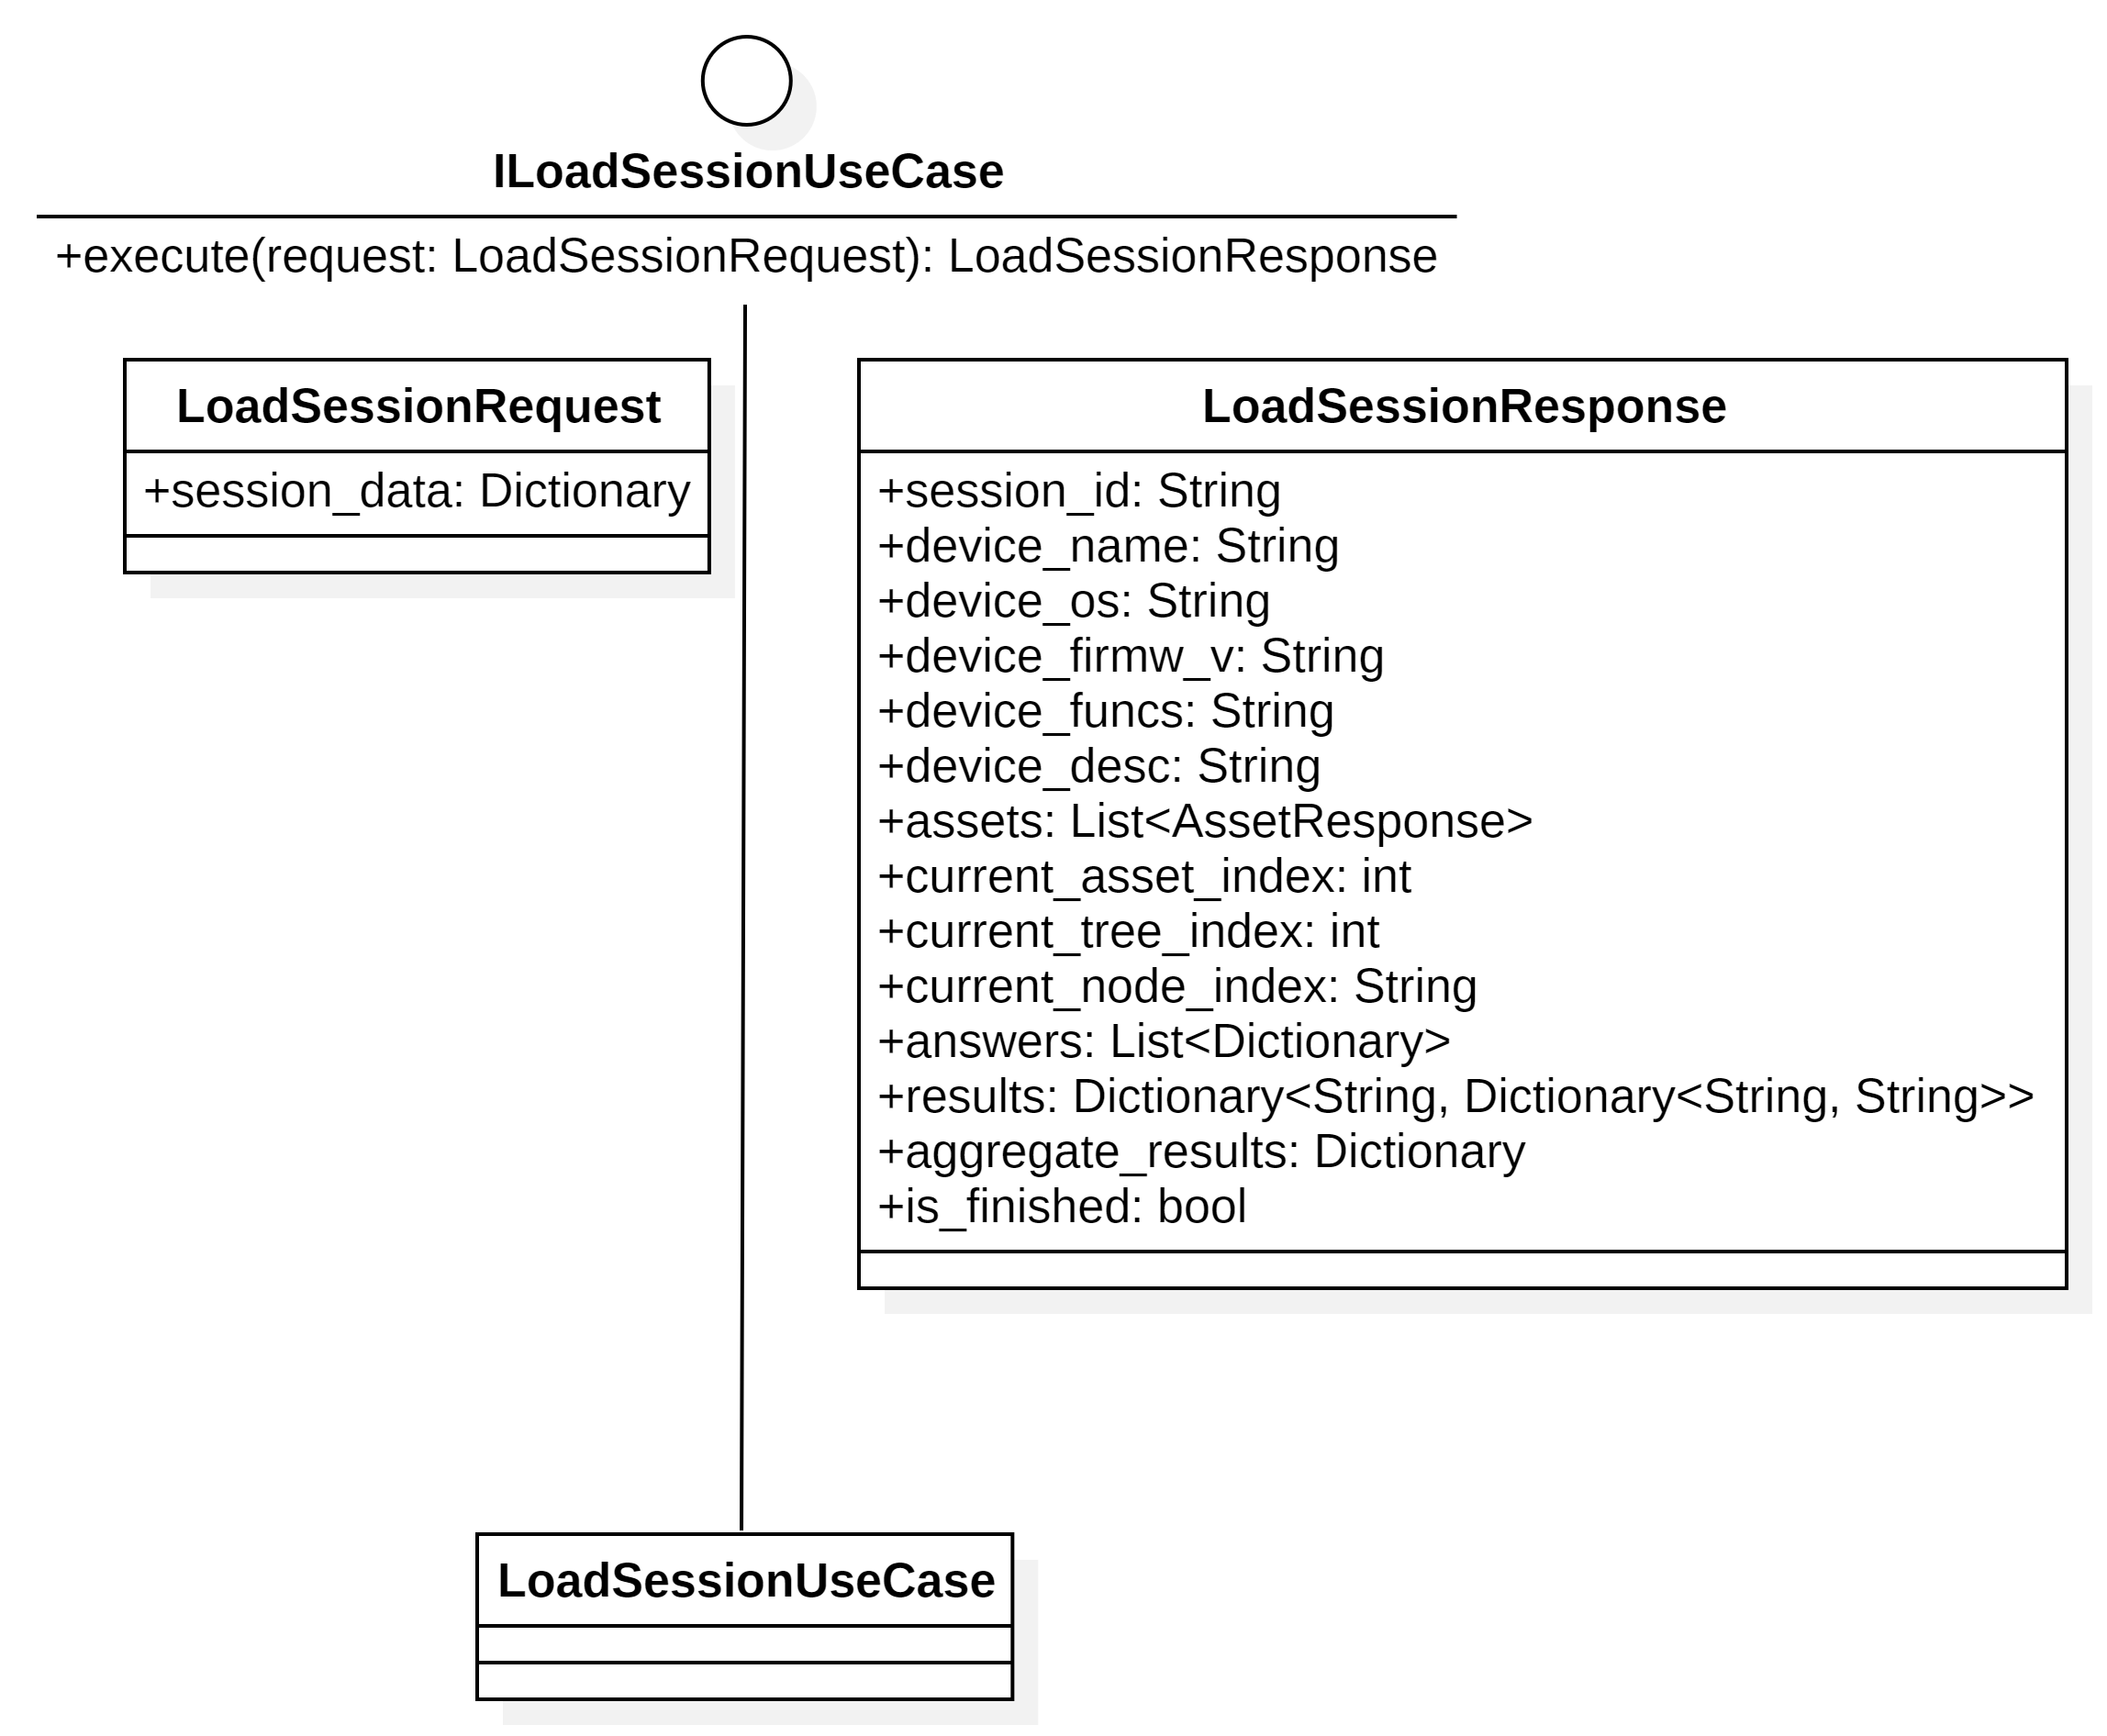
\includegraphics[width=.8\linewidth]{../../../Assets/Classi/LoadSessionUC.png}
                              \caption{ILoadSessionUseCase: interfaccia, DTOs e classe}
                        \end{figure}
                    \end{center}
                    

                \paragraph{LoadSessionRequest}\mbox{}\\
                    DTO di richiesta per l'upload della sessione.\\\\
                    \textbf{Attributi}
                    \begin{itemize}
                        \item {\ttfamily session\_data: Dictionary}: dizionario contenente le informazioni della sessione.
                    \end{itemize}

                \paragraph{LoadSessionResponse}\mbox{}\\
                    DTO di risposta all'upload della sessione.\\\\
                    \textbf{Attributi}
                    \begin{itemize}
                        \item {\ttfamily session\_id: String}: id univoco della sessione;
                        \item {\ttfamily device\_name: String}: nome del dispositivo oggetto di verifica;
                        \item {\ttfamily device\_os: String}, {\ttfamily device\_firmw\_v: String}, {\ttfamily device\_funcs: String}, {\ttfamily device\_desc: String}: metadati relativi al dispositivo;
                        \item {\ttfamily assets: list<AssetResponse>}: \textit{lista}\textsubscript{\href{https://atlasteam9.github.io/Atlas/glossario.html\#Lista}{G}} degli asset del dispositivo;
                        \item {\ttfamily current\_asset\_index: int}: indice dell'asset corrente;
                        \item {\ttfamily current\_tree\_index: int}: indice dell'albero corrente;
                        \item {\ttfamily current\_node\_id: String}: id del \textit{nodo}\textsubscript{\href{https://atlasteam9.github.io/Atlas/glossario.html\#Nodo}{G}} corrente.
                        \item {\ttfamily answers: list<Dictionary>}: \textit{lista}\textsubscript{\href{https://atlasteam9.github.io/Atlas/glossario.html\#Lista}{G}} delle riposte date nel precedente test della sessione.
                        \item {\ttfamily results: Dictionary<String, Dictionary<String, String>}: dizionario contenente i risultati di ogni \textit{requisito}\textsubscript{\href{https://atlasteam9.github.io/Atlas/glossario.html\#Requisito}{G}} per ogni asset. 
                        \item {\ttfamily aggregate\_results: Dictionary}: dizionario dei risultati con formato utile al frontend per la visualizzazione
                        \item {\ttfamily is\_finished: bool}: valore booleano che dice se la sessione caricata era conclusa o meno
                    \end{itemize}


                \paragraph{LoadSessionUseCase}\mbox{}\\
                    Carica una vecchia sessione salvata su file e ripristina il contesto, mostrando tutti i risultati già ottenuti.\\\\
                    \textbf{Attributo}
                    \begin{itemize}
                        \item {\ttfamily \_session\_service: ISessionService}
                        \item {\ttfamily \_factory: SessionFactory}
                    \end{itemize}
                    \textbf{Metodo}
                    \begin{itemize}
                        \item {\ttfamily execute(request: LoadSessionRequest): LoadSessionResponse}
                    \end{itemize}

                \paragraph{IGetTreesUseCase}\mbox{}\\
                    Contratto per il recupero della \textit{lista}\textsubscript{\href{https://atlasteam9.github.io/Atlas/glossario.html\#Lista}{G}} degli alberi decisionali disponibili.

                    \begin{center}
                        \begin{figure}[H]
                              \centering
                              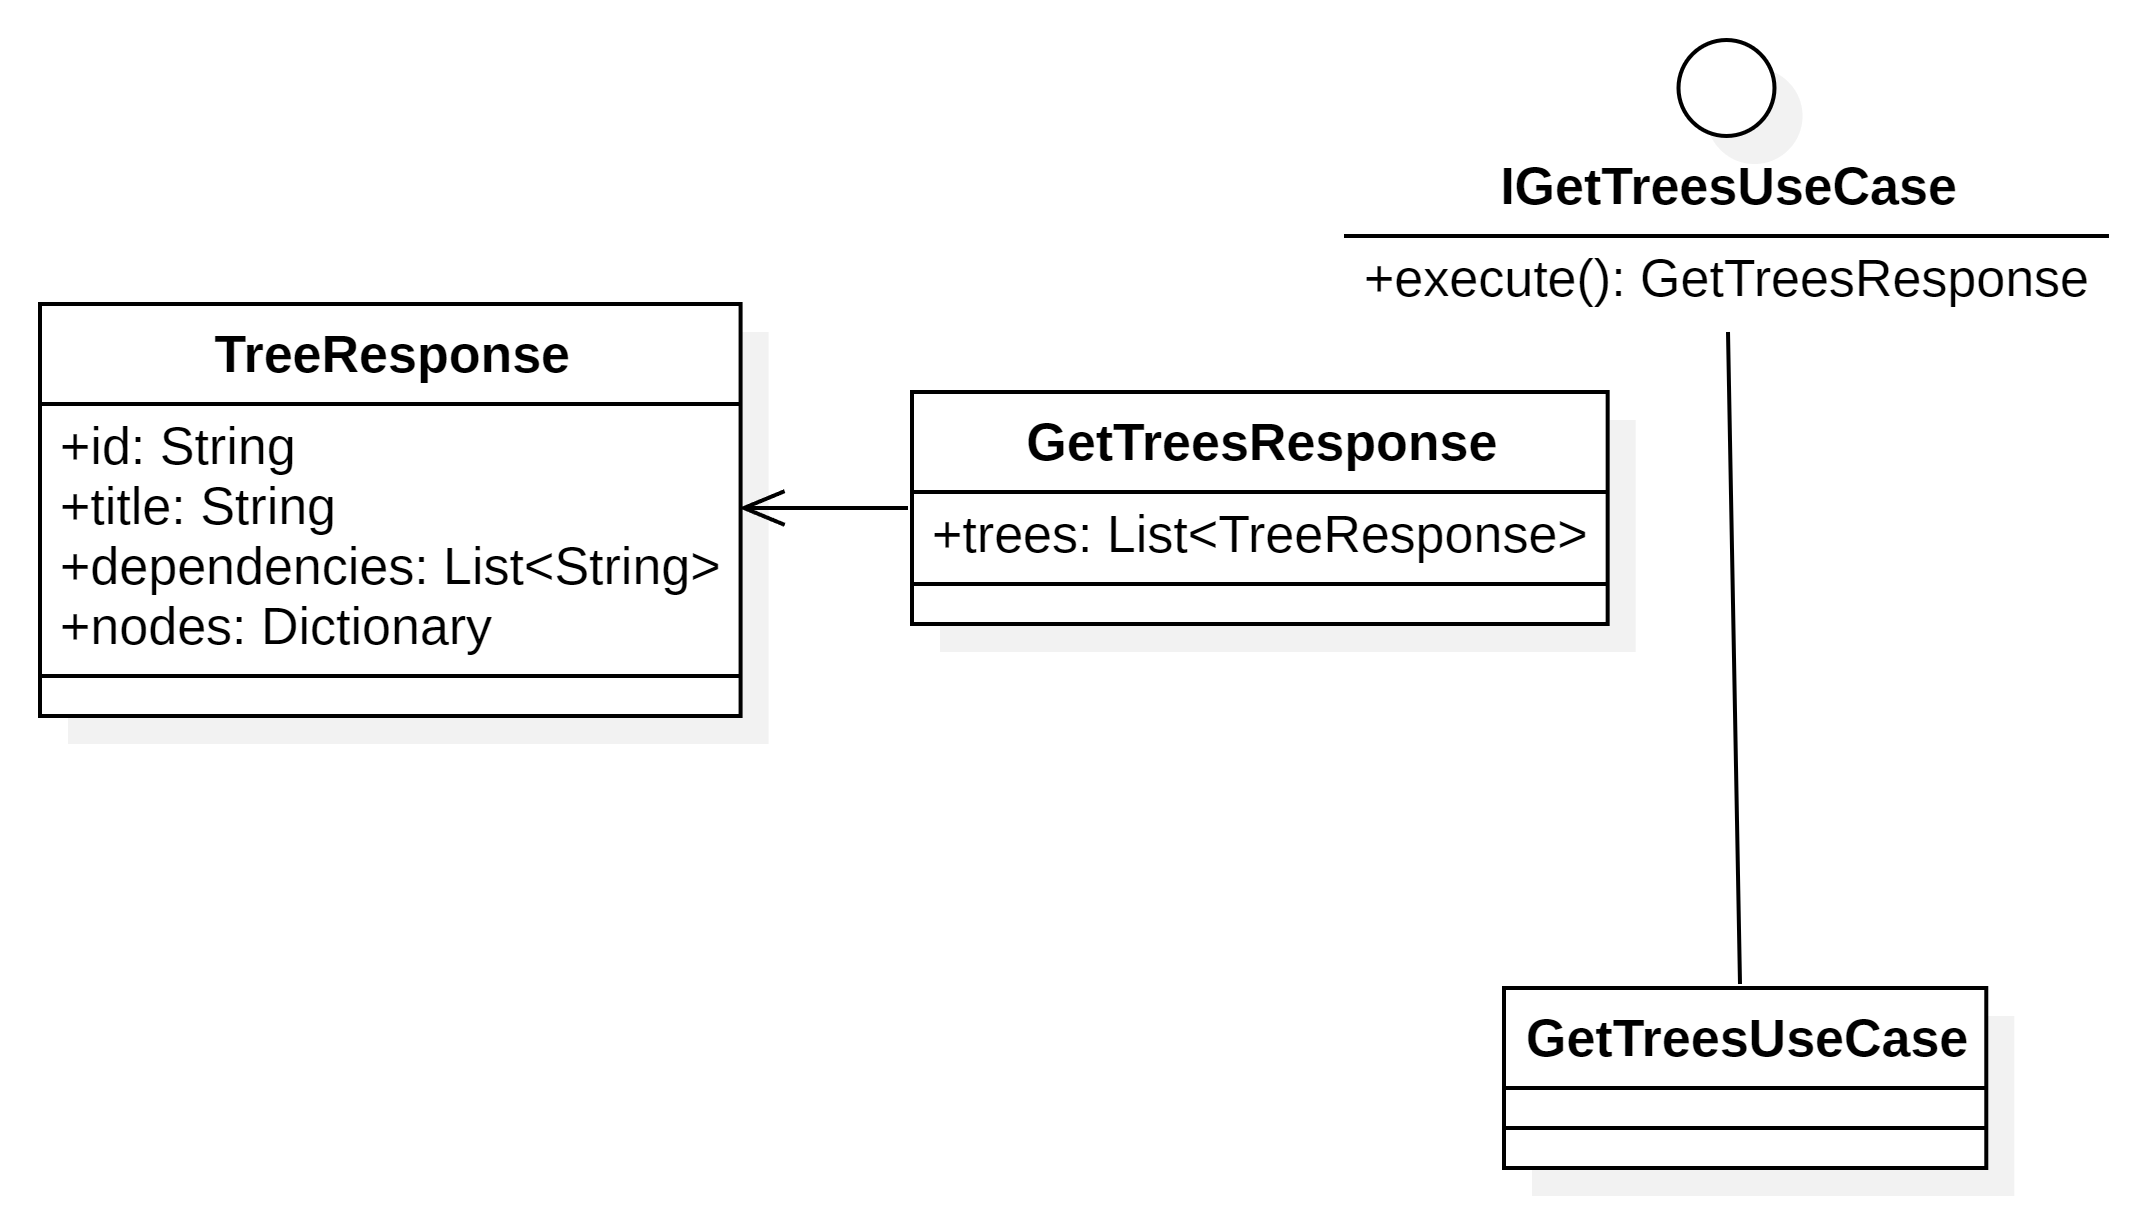
\includegraphics[width=.6\linewidth]{../../../Assets/Classi/GetTreesUC.png}
                              \caption{GetTreesUseCase: interfaccia, DTOs e classe}
                        \end{figure}
                    \end{center}

                \paragraph{TreesResponse}\mbox{}\\
                    DTO di risposta che ritorna un singolo albero decisionali.\\\\
                    \textbf{Attributi}
                    \begin{itemize}
                        \item {\ttfamily id: String}: id dell'albero;
                        \item {\ttfamily title: String}: titolo dell'albero;
                        \item {\ttfamily dependencies: list<String>}: dipendenze dell'albero;
                        \item {\ttfamily nodes: Dictionary}: nodi dell'albero.
                    \end{itemize}

                \paragraph{GetTreesResponse}\mbox{}\\
                    DTO di risposta che ritorna la \textit{lista}\textsubscript{\href{https://atlasteam9.github.io/Atlas/glossario.html\#Lista}{G}} di alberi decisionali.\\\\
                    \textbf{Attributi}
                    \begin{itemize}
                        \item {\ttfamily trees: list<TreesResponse>}: \textit{lista}\textsubscript{\href{https://atlasteam9.github.io/Atlas/glossario.html\#Lista}{G}} di alberi.
                    \end{itemize}


                \paragraph{GetTreesUseCase}\mbox{}\\
                    Riceve la \textit{lista}\textsubscript{\href{https://atlasteam9.github.io/Atlas/glossario.html\#Lista}{G}} di alberi caricata in memoria e la serializza come \textit{lista}\textsubscript{\href{https://atlasteam9.github.io/Atlas/glossario.html\#Lista}{G}} di dizionari.\\\\
                    \textbf{Metodo}
                    \begin{itemize}
                        \item {\ttfamily execute(): GetTreesResponse}: ritorna una \textit{lista}\textsubscript{\href{https://atlasteam9.github.io/Atlas/glossario.html\#Lista}{G}} di alberi.
                    \end{itemize}
            
                \paragraph{ISessionService}\mbox{}\\
                    \textit{Interfaccia}\textsubscript{\href{https://atlasteam9.github.io/Atlas/glossario.html\#Interfaccia}{G}} del service di dominio esposta verso l'application layer.\\\\

                    \begin{center}
                        \begin{figure}[H]
                              \centering
                              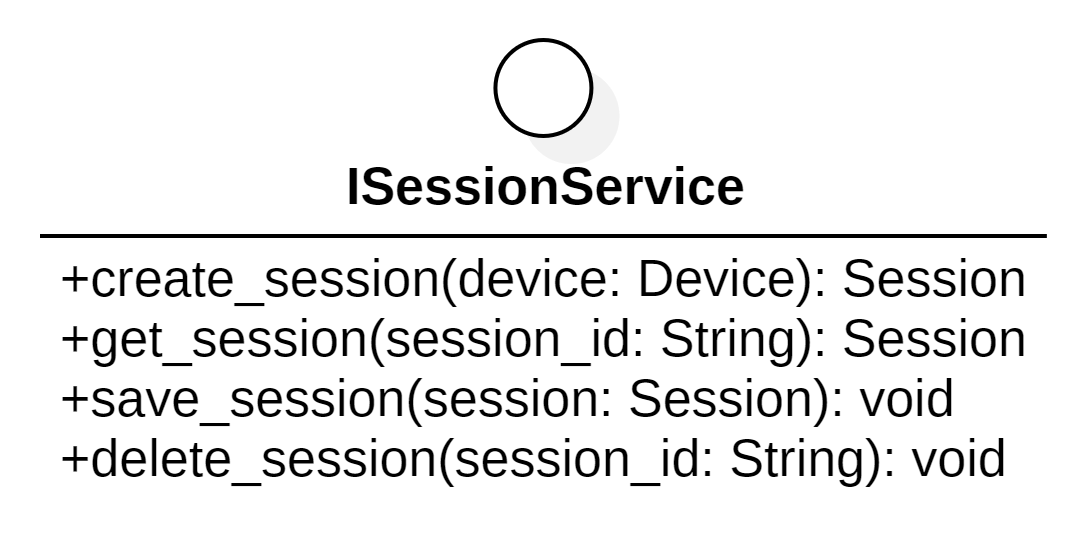
\includegraphics[width=.6\linewidth]{../../../Assets/Classi/ISessionService.png}
                              \caption{ISessionService: interfaccia}
                        \end{figure}
                    \end{center}
                    
                    \textbf{Metodi}
                    \begin{itemize}
                        \item {\ttfamily create\_session(device: Device): Session}: crea una session a partire dal dispositivo passato per parametro;
                        \item {\ttfamily get\_session(session\_id: String): Session | null}: recupera la sessione con l'id passato per parametro dalla repo;
                        \item {\ttfamily save\_session(session: Session): null}: salva la sessione passata per parametro;
                        \item {\ttfamily delete\_session(session\_id: String): null}: elimina la sessione con l'id passato per parametro.
                    \end{itemize}
                    
            \subsubsection{Domain Layer}
                \textbf{Scopo}: Rappresenta il cuore pulsante del sistema, contenente le regole di business fondamentali.

                \noindent\textbf{Responsabilità}: Definisce le entità (come Session, Device, DecisionTree) e la logica che non dipende da \textit{framework}\textsubscript{\href{https://atlasteam9.github.io/Atlas/glossario.html\#Framework}{G}} o database. È il layer più interno e isolato.

                \paragraph{AssetType}

                    \begin{center}
                        \begin{figure}[H]
                              \centering
                              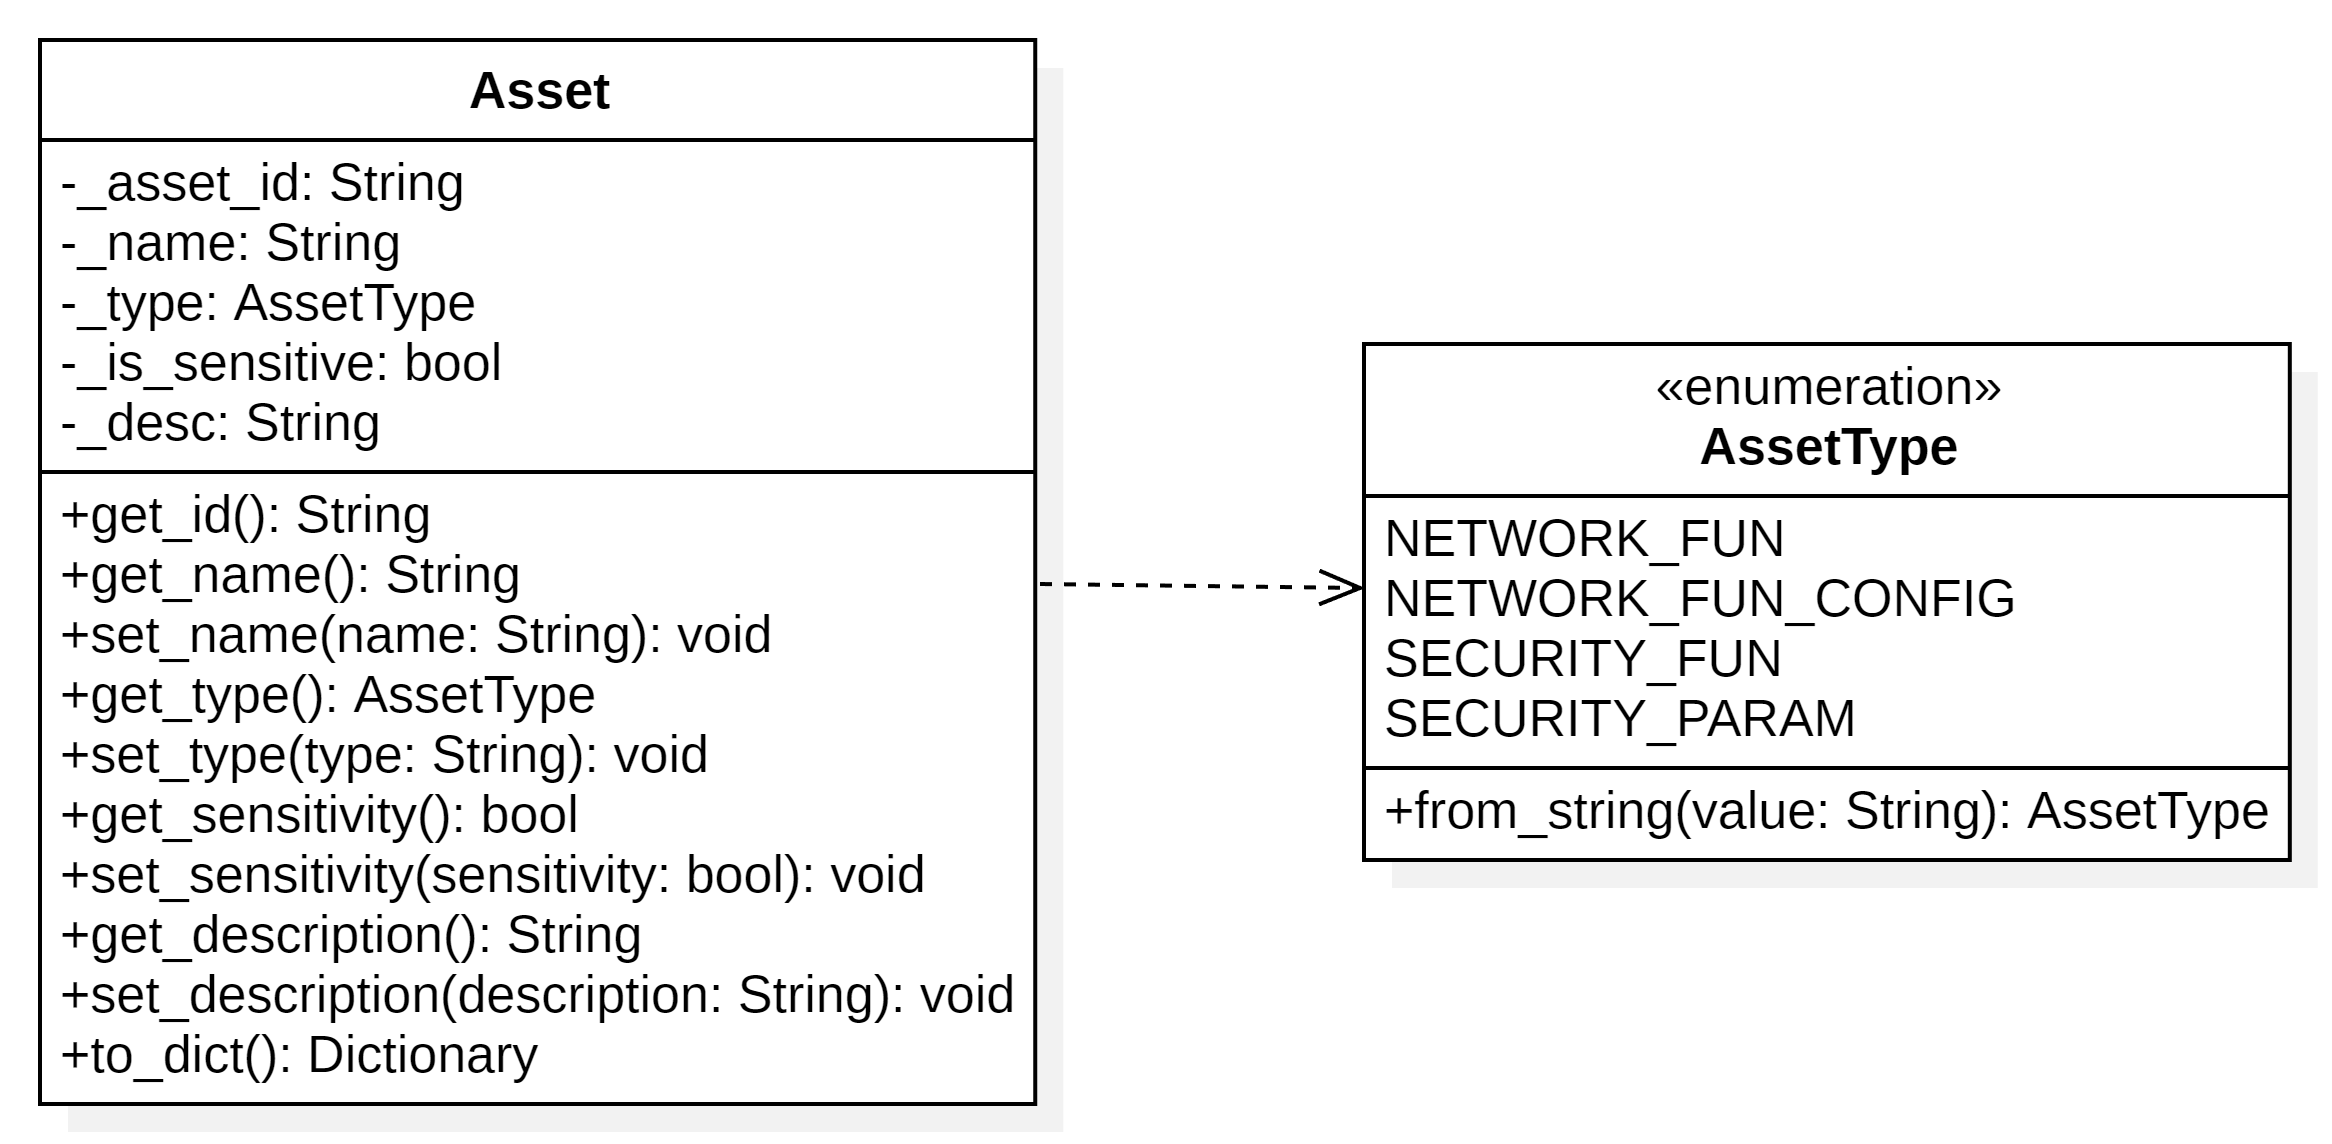
\includegraphics[width=.8\linewidth]{../../../Assets/Classi/Asset.png}
                              \caption{Asset: classe e relativa enumerazione}
                        \end{figure}
                    \end{center}
                    
                    Enumerazione che defnisce i quattro asset previsti dallo standard EN18031:
                    \begin{itemize}
                        \item Network function;
                        \item Network function configuration;
                        \item Security function;
                        \item Securitfy parameter.
                    \end{itemize}
                    Espone un metodo di classe {\ttfamily from\_string(value: String): AssetType}, per costruire il valore corretto a partire da una stringa. 

                    Un metodo di classe in Python è un metodo che riceve la classe stessa come primo parametro implicito, mentre un metodo di istanza riceve l'istanza.

                        
                \paragraph{Asset}\mbox{}\\
                    Rappresenta un singolo componente da testare.\\\\
                    \textbf{Attributi}
                    \begin{itemize}
                        \item {\ttfamily \_asset\_id: String}: id univoco dell'asset;
                        \item {\ttfamily \_name: String}: nome dell'asset;
                        \item {\ttfamily \_type: AssetType}: tipo dell'asset;
                        \item {\ttfamily \_is\_sensitive: bool}: flag di sensibilità dell'asset;
                        \item {\ttfamily \_desc: String}: descrizione (opzionale) dell'asset.
                    \end{itemize}
                    \textbf{Metodi}
                        \begin{itemize}
                            \item Metodi getter per ogni attributo;
                            \item Metodi setter per ogni attributo ad eccezione dell'id;
                            \item {\ttfamily to\_dict(): Dictionary}: metodo utilizzato per la serializzazione.
                        \end{itemize}
                \paragraph{Device}\mbox{}\\

                    \begin{center}
                        \begin{figure}[H]
                              \centering
                              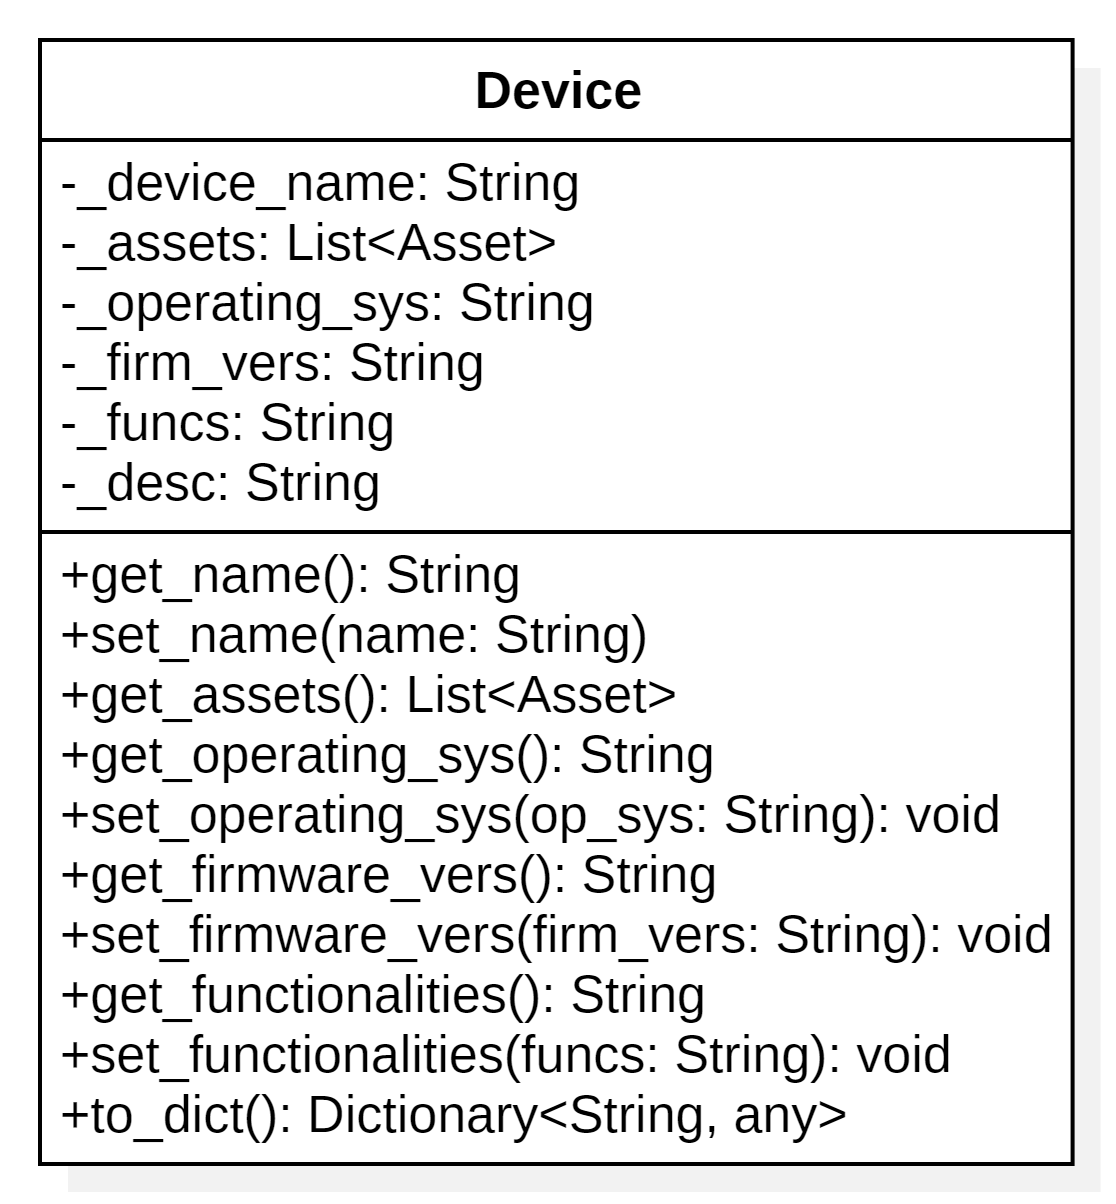
\includegraphics[width=.4\linewidth]{../../../Assets/Classi/Device.png}
                              \caption{Device: classe}
                        \end{figure}
                    \end{center}
                    
                    Rappresenta il dispositivo facente uso di onde radio oggetto della valutazione. Aggrega una \textit{lista}\textsubscript{\href{https://atlasteam9.github.io/Atlas/glossario.html\#Lista}{G}} di Asset e contiene le informazioni generali del dispositivo.\\\\
                    \textbf{Attributi}
                    \begin{itemize}
                        \item {\ttfamily \_device\_name: String}: nome del dispositivo;
                        \item {\ttfamily \_assets: list<Asset>}: \textit{lista}\textsubscript{\href{https://atlasteam9.github.io/Atlas/glossario.html\#Lista}{G}} degli asset;
                        \item {\ttfamily \_operating\_sys: String}: sistema operativo del dispositivo;
                        \item {\ttfamily \_firm\_vers: String}: versione del \textit{firmware}\textsubscript{\href{https://atlasteam9.github.io/Atlas/glossario.html\#Firmware}{G}} del dispositivo;
                        \item {\ttfamily \_funcs: String}: funzionalità del dispositivo;
                        \item {\ttfamily \_desc: String}: descrizione del dispositivo.
                    \end{itemize}
                    \textbf{Metodi}
                        \begin{itemize}
                            \item Metodi getter per ogni attributo;
                            \item Metodi setter per ogni attributo ad eccezione della \textit{lista}\textsubscript{\href{https://atlasteam9.github.io/Atlas/glossario.html\#Lista}{G}} degli asset;
                            \item {\ttfamily to\_dict(): Dictionary<String, any>}: metodo utilizzato per la serializzazione.
                        \end{itemize}
                
                \paragraph{Node}\mbox{}\\

                    \begin{center}
                        \begin{figure}[H]
                              \centering
                              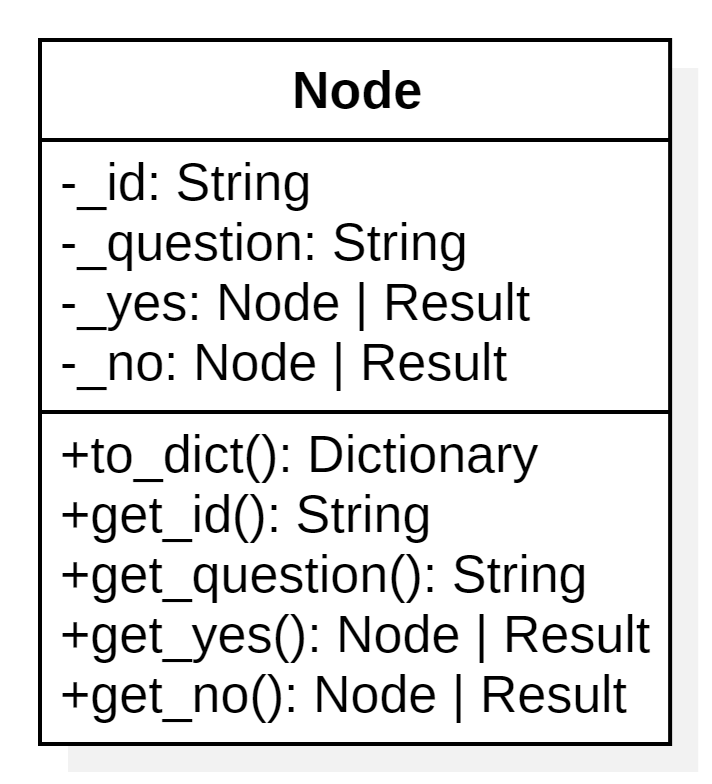
\includegraphics[width=.2\linewidth]{../../../Assets/Classi/Node.png}
                              \caption{Node: classe}
                        \end{figure}
                    \end{center}
                    
                    Rappresenta un \textit{nodo}\textsubscript{\href{https://atlasteam9.github.io/Atlas/glossario.html\#Nodo}{G}} di un decision tree.\\\\
                    \textbf{Attributi}
                    \begin{itemize}
                        \item {\ttfamily \_node\_id: String}: id del \textit{nodo}\textsubscript{\href{https://atlasteam9.github.io/Atlas/glossario.html\#Nodo}{G}};
                        \item {\ttfamily \_question: String}: stringa contenente il testo della domanda;
                        \item {\ttfamily \_yes: Node | Result}: risposta "sì", può portare ad un altro \textit{nodo}\textsubscript{\href{https://atlasteam9.github.io/Atlas/glossario.html\#Nodo}{G}} o a un risultato;
                        \item {\ttfamily \_no: Node | Result}: risposta "no", può portare ad un altro \textit{nodo}\textsubscript{\href{https://atlasteam9.github.io/Atlas/glossario.html\#Nodo}{G}} o a un risultato;
                    \end{itemize}
                    \textbf{Metodi}
                        \begin{itemize}
                            \item Metodi getter per ogni attributo.
                            \item {\ttfamily to\_dict(): Dictionary}: utilizzato per la serializzazione.
                        \end{itemize}
                \paragraph{DecisionTree}\mbox{}\\

                    \begin{center}
                        \begin{figure}[H]
                              \centering
                              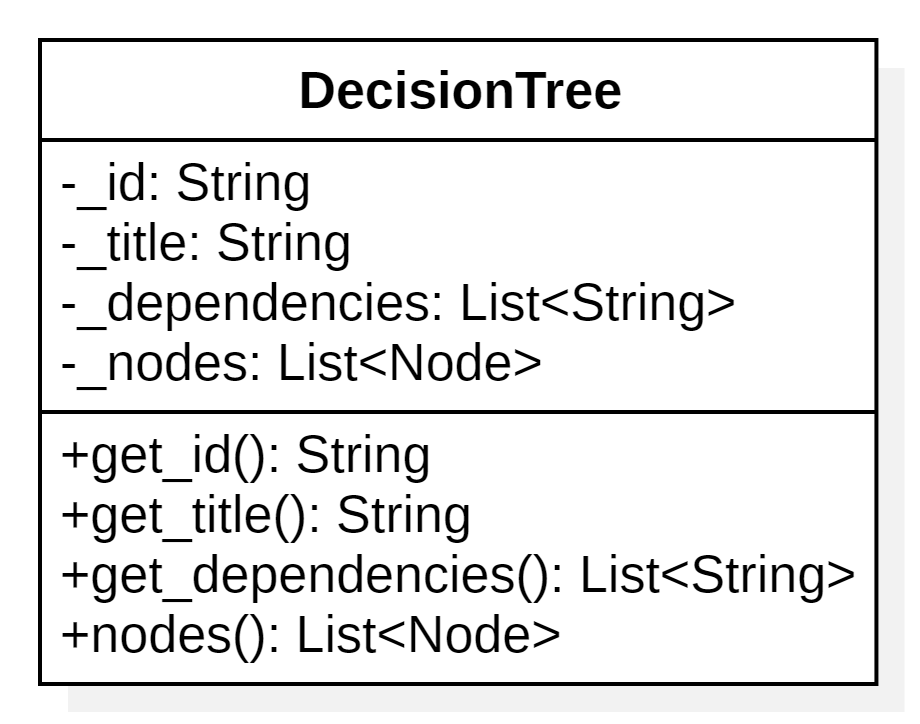
\includegraphics[width=.3\linewidth]{../../../Assets/Classi/DecisionTree.png}
                              \caption{DecisionTree: classe}
                        \end{figure}
                    \end{center}
                    
                    Albero decisionale corrispondente ad un \textit{requisito}\textsubscript{\href{https://atlasteam9.github.io/Atlas/glossario.html\#Requisito}{G}} EN 18031. l'iterazione diretta sui nodi serializzati.\\\\
                    \textbf{Attributi}
                    \begin{itemize}
                        \item {\ttfamily \_id: String}: id dell'albero;
                        \item {\ttfamily \_title: String}: titolo dell'albero;
                        \item {\ttfamily \_dependencies: list[String]}: \textit{lista}\textsubscript{\href{https://atlasteam9.github.io/Atlas/glossario.html\#Lista}{G}} delle dipendenze dell'albero;
                        \item {\ttfamily \_nodes: list[Node]}: \textit{lista}\textsubscript{\href{https://atlasteam9.github.io/Atlas/glossario.html\#Lista}{G}} contenente i nodi del decision tree.
                    \end{itemize}
                    \textbf{Metodi}
                        \begin{itemize}
                            \item Metodi getter per ogni attributo.
                        \end{itemize}

                        
                \paragraph{Session}\mbox{}\\

                    \begin{center}
                        \begin{figure}[H]
                              \centering
                              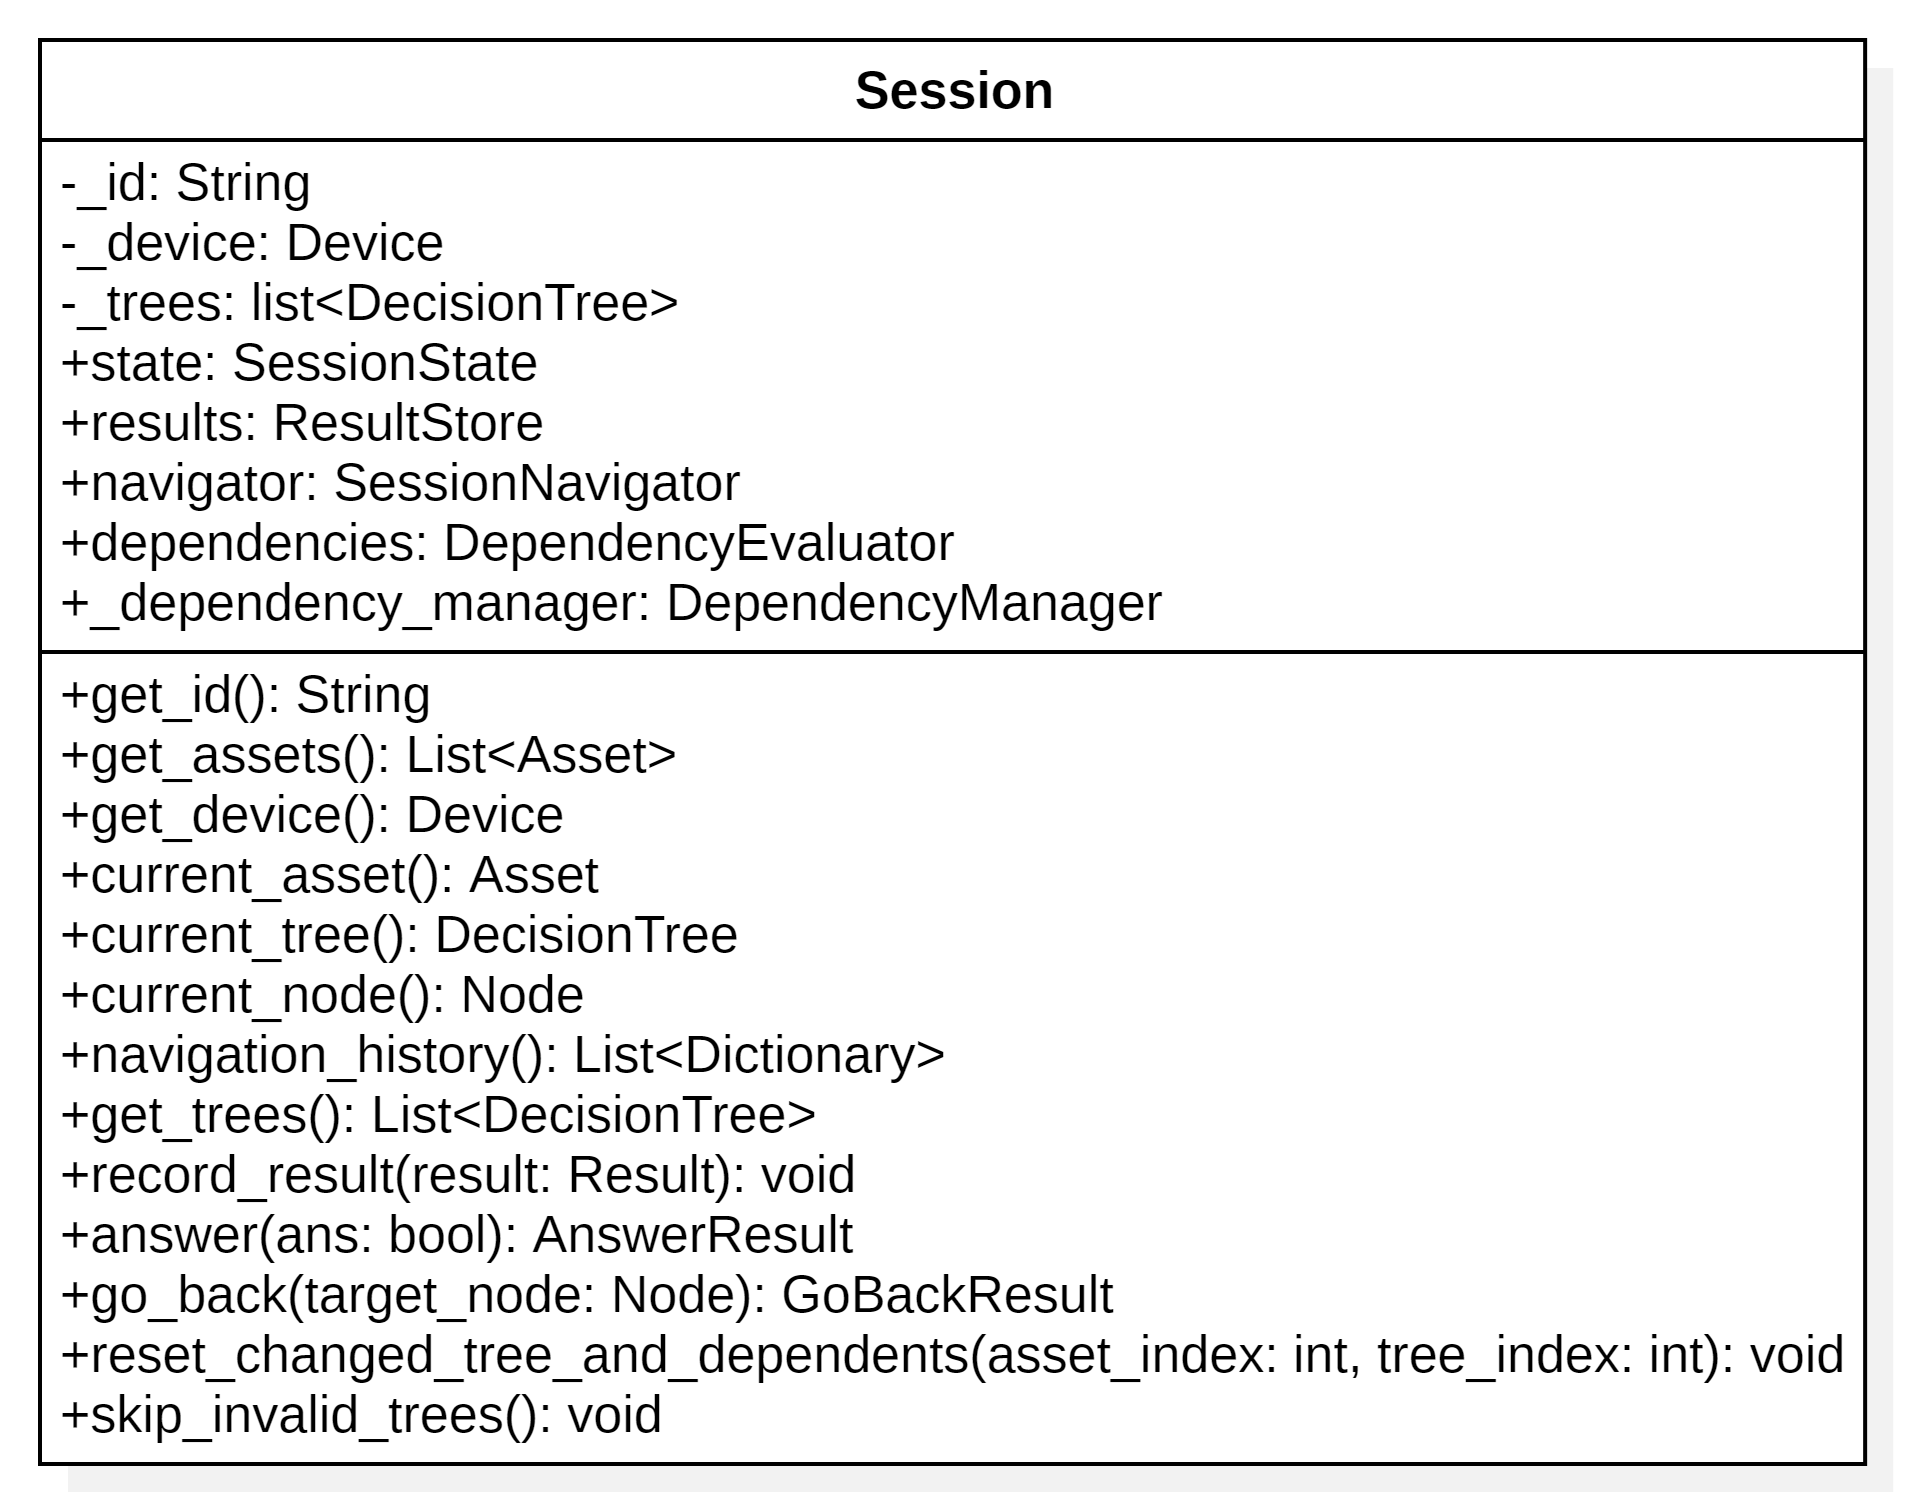
\includegraphics[width=.6\linewidth]{../../../Assets/Classi/Session.png}
                              \caption{Session: classe}
                        \end{figure}
                    \end{center}
                    
                    Aggregato radice che rappresenta una sessione di test in corso. Contiene lo stato e la logica per l'avanzamento.\\\\
                    \textbf{Attributi}
                    \begin{itemize}
                        \item {\ttfamily \_id: String}: id della sessione;
                        \item {\ttfamily \_device: Device}: dispositivo associato alla sessione;
                        \item {\ttfamily \_trees: list[DecisionTree]}: \textit{lista}\textsubscript{\href{https://atlasteam9.github.io/Atlas/glossario.html\#Lista}{G}} degli alberi;
                        \item {\ttfamily state: SessionState}: stato corrente della sessione;
                        \item {\ttfamily results: ResultStore}: registratore dei risultati;
                        \item {\ttfamily navigator: SessionNavigator}: navigatore della sessione;
                        \item {\ttfamily dependencies: DependencyEvaluator}: controllore delle dipendenze;
                        \item {\ttfamily \_dependency\_manager: DependencyManager}: gestore delle regole di dipendenza fra i decision tree.
                    \end{itemize}
                    \textbf{Metodi}
                        \begin{itemize}
                            \item Metodi getter per: id, \textit{lista}\textsubscript{\href{https://atlasteam9.github.io/Atlas/glossario.html\#Lista}{G}} completa degli asset, asset corrente, dispositivo, albero corrente, \textit{nodo}\textsubscript{\href{https://atlasteam9.github.io/Atlas/glossario.html\#Nodo}{G}} corrente, storia di navigazione, \textit{lista}\textsubscript{\href{https://atlasteam9.github.io/Atlas/glossario.html\#Lista}{G}} completa degli alberi;
                            \item {\ttfamily record\_result(result: Result): void}: registra il risultato di un \textit{decision tree}\textsubscript{\href{https://atlasteam9.github.io/Atlas/glossario.html\#DecisionTree}{G}};
                            \item {\ttfamily answer(ans: bool): AnswerResult}: gestisce la risposta ad una domanda di un \textit{nodo}\textsubscript{\href{https://atlasteam9.github.io/Atlas/glossario.html\#Nodo}{G}};
                            \item {\ttfamily go\_back(target\_node: Node): GoBackResult}: ritorna indietro alla risposta di un \textit{nodo}\textsubscript{\href{https://atlasteam9.github.io/Atlas/glossario.html\#Nodo}{G}} target;
                            \item {\ttfamily reset\_changed\_tree\_and\_dependents(asset\_index: int,  tree\_index: int): void}: resetta le dipendenze in caso di modifica di una risposta ad un \textit{decision tree}\textsubscript{\href{https://atlasteam9.github.io/Atlas/glossario.html\#DecisionTree}{G}};
                            \item {\ttfamily \_skip\_invalid\_trees(): void}: se le dipendenze non sono soddisfatte salta l'albero.
                        \end{itemize}

            
                    \paragraph{SessionService}

                    \begin{center}
                        \begin{figure}[H]
                              \centering
                              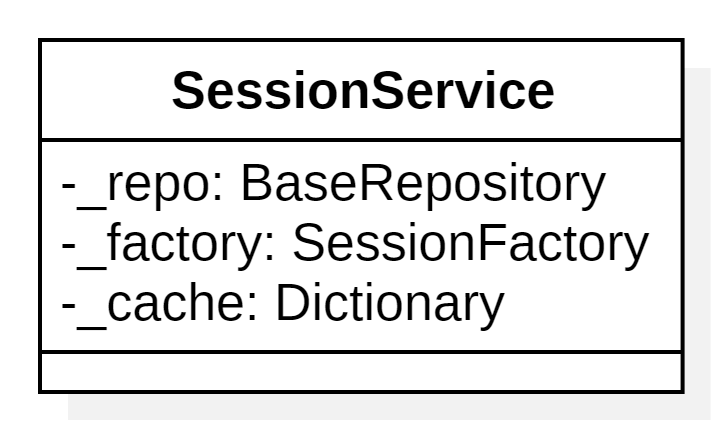
\includegraphics[width=.4\linewidth]{../../../Assets/Classi/SessionService.png}
                              \caption{SessionService: classe}
                        \end{figure}
                    \end{center}
                    
                    Implementazione concreta di ISessionService. Coordina la creazione, il recupero, il salvataggio e la cancellazione delle sessioni.\\\\
                    \textbf{Attributi}
                    \begin{itemize}
                        \item {\ttfamily \_repo: BaseRepository}: \textit{interfaccia}\textsubscript{\href{https://atlasteam9.github.io/Atlas/glossario.html\#Interfaccia}{G}} generica e astratta che definisce il contratto standard (operazioni di salvataggio, recupero e cancellazione) per la persistenza delle entità
                        \item {\ttfamily \_factory: SessionFactory}: factory che centralizza la costruzione di oggetti Session;
                        \item {\ttfamily \_cache: Dictionary}: cache usata per evitare di ricaricare dal file system sessioni già attive nella stessa request;
                    \end{itemize}
                    \textbf{Metodi}\\
                        La classe implementa i metodi dichiarati dall'\textit{interfaccia}\textsubscript{\href{https://atlasteam9.github.io/Atlas/glossario.html\#Interfaccia}{G}} {\ttfamily ISessionService}.

                        
                \paragraph{SessionState}\mbox\\

                    \begin{center}
                        \begin{figure}[H]
                              \centering
                              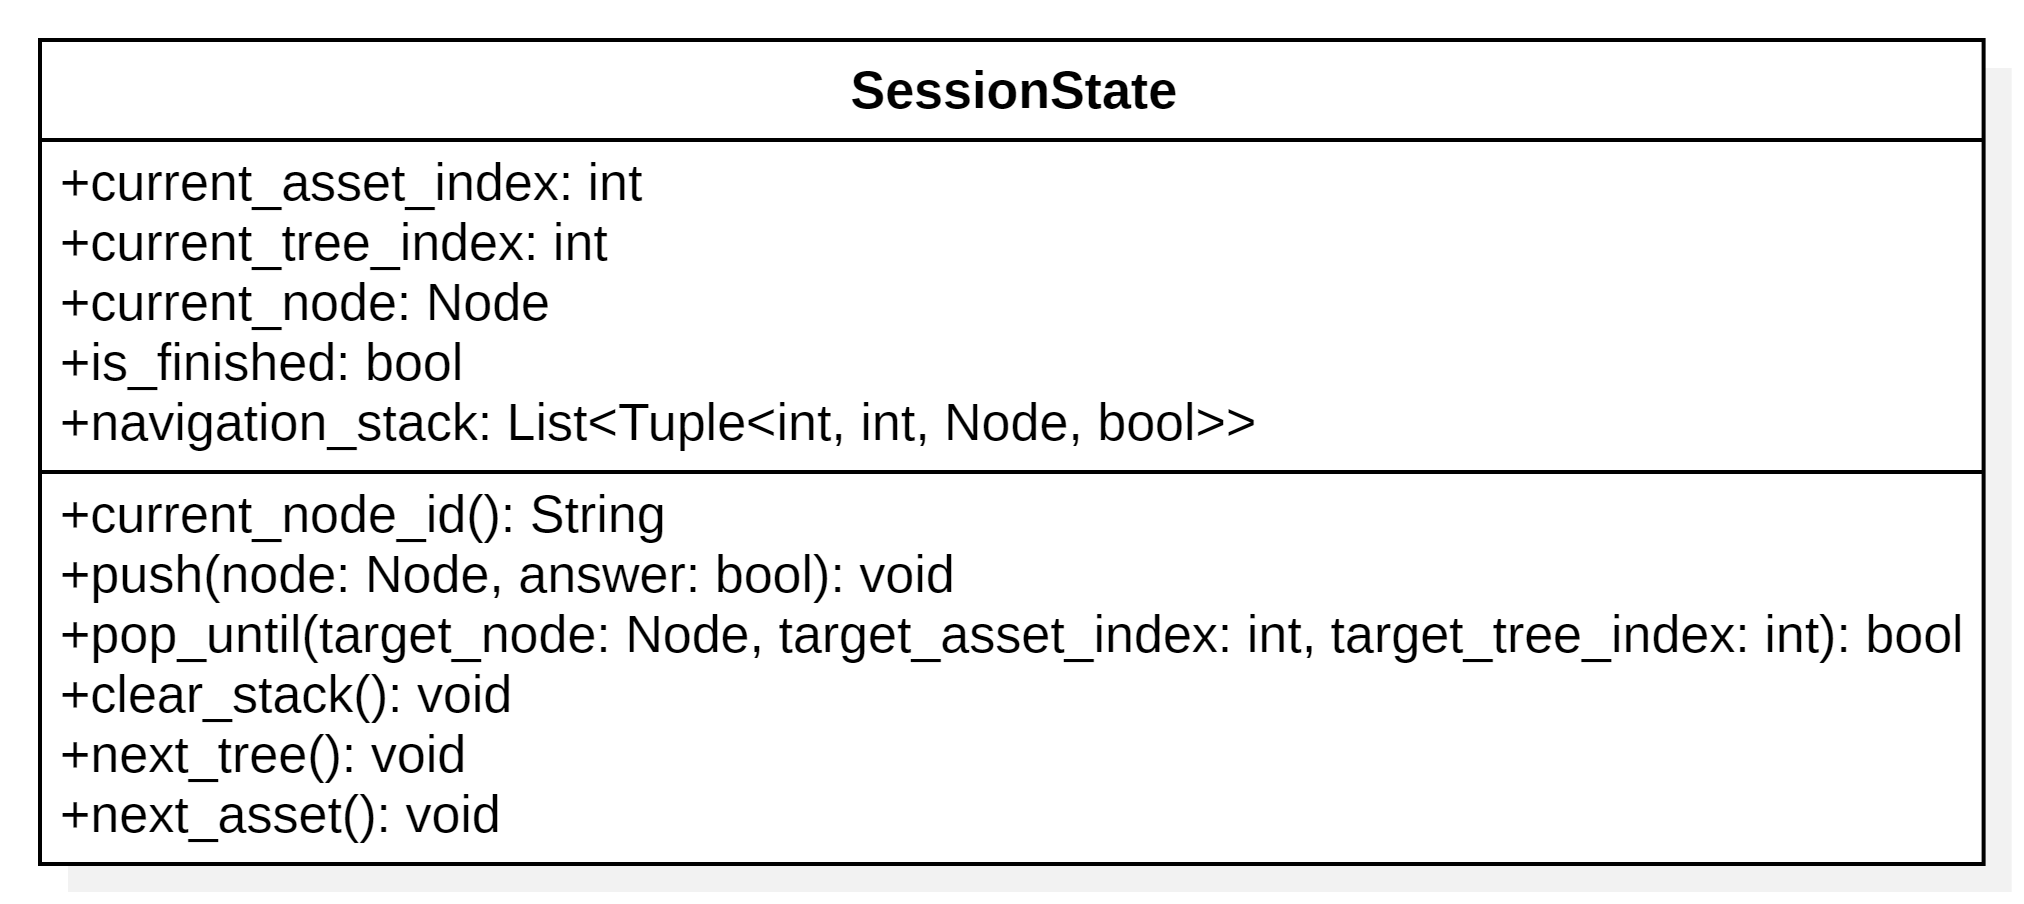
\includegraphics[width=.6\linewidth]{../../../Assets/Classi/SessionState.png}
                              \caption{SessionState: classe}
                        \end{figure}
                    \end{center}

                    Contenitore dello stato serializzabile della sessione. Fornisce i metodi per manipolare lo stack e avanzare tra alberi e asset.\\\\
                    \textbf{Attributi}
                    \begin{itemize}
                        \item {\ttfamily current\_asset\_index: int}: indice dell'asset corrente;
                        \item {\ttfamily current\_tree\_index: int}: indice del \textit{decision tree}\textsubscript{\href{https://atlasteam9.github.io/Atlas/glossario.html\#DecisionTree}{G}} corrente;
                        \item {\ttfamily current\_node: Node}: \textit{nodo}\textsubscript{\href{https://atlasteam9.github.io/Atlas/glossario.html\#Nodo}{G}} corrente;
                        \item {\ttfamily is\_finished: bool}: flag di completamento;
                        \item {\ttfamily navigation\_stack: list$<$tuple$<$int, Node, bool$>>$}: stack di navigazione. Una \textit{lista}\textsubscript{\href{https://atlasteam9.github.io/Atlas/glossario.html\#Lista}{G}} di tuple composte da tre elementi: l'indice dell'albero, il \textit{nodo}\textsubscript{\href{https://atlasteam9.github.io/Atlas/glossario.html\#Nodo}{G}} a cui si ha risposto, la risposta data. 
                    \end{itemize}
                    \textbf{Metodi}
                    \begin{itemize}
                        \item {\ttfamily current\_node\_id(): String}: ritorna l'id del \textit{nodo}\textsubscript{\href{https://atlasteam9.github.io/Atlas/glossario.html\#Nodo}{G}} corrente;
                        \item {\ttfamily \textit{push}\textsubscript{\href{https://atlasteam9.github.io/Atlas/glossario.html\#Push}{G}}(node: Node, answer: bool): void}: pusha in coda allo stack di navigazione la coppia nodo-risposta;
                        \item {\ttfamily pop\_until(target\_node: Node, target\_asset\_index: int, target\_tree\_index: int): bool}: rimuove dallo stack tutte le entry dal fondo fino al \textit{nodo}\textsubscript{\href{https://atlasteam9.github.io/Atlas/glossario.html\#Nodo}{G}} target compreso. Ritorna true o false in base alla presenza del \textit{nodo}\textsubscript{\href{https://atlasteam9.github.io/Atlas/glossario.html\#Nodo}{G}} nello stack;
                        \item {\ttfamily clear\_stack(): void}: svuota lo stack;
                        \item {\ttfamily next\_tree(): void}: avanza al prossimo albero;
                        \item {\ttfamily next\_asset(): void}: avanza al prossimo asset.
                    \end{itemize}

                    
                \paragraph{AnswerResult}\mbox{}\\

                    \begin{center}
                        \begin{figure}[H]
                              \centering
                              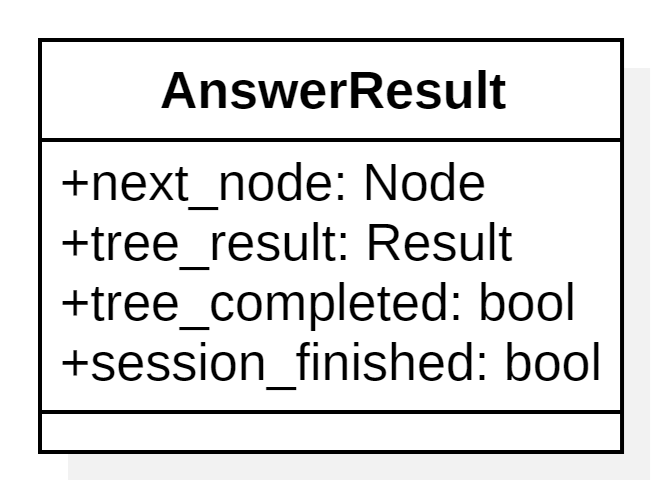
\includegraphics[width=.4\linewidth]{../../../Assets/Classi/AnswerResult.png}
                              \caption{AnswerResult: classe}
                        \end{figure}
                    \end{center}
                    
                    Value object resitutito da SessionNavigator.answer(). Porta il prossimo \textit{nodo}\textsubscript{\href{https://atlasteam9.github.io/Atlas/glossario.html\#Nodo}{G}} se il tree continua, il risultato e il flag tree\_completed se il tree è terminato e session\_finished se tutti gli asset e alberi sono stati completati.\\\\
                    \textbf{Attributi}
                    \begin{itemize}
                        \item {\ttfamily next\_node: Node}: prossimo \textit{nodo}\textsubscript{\href{https://atlasteam9.github.io/Atlas/glossario.html\#Nodo}{G}};
                        \item {\ttfamily tree\_result: Result}: risultato dell'albero;
                        \item {\ttfamily tree\_completed: bool}: flag di albero completato;
                        \item {\ttfamily session\_finished: bool}: flag di fine sessione.
                    \end{itemize}

                    
                \paragraph{GoBackResult}\mbox{}\\

                    \begin{center}
                        \begin{figure}[H]
                              \centering
                              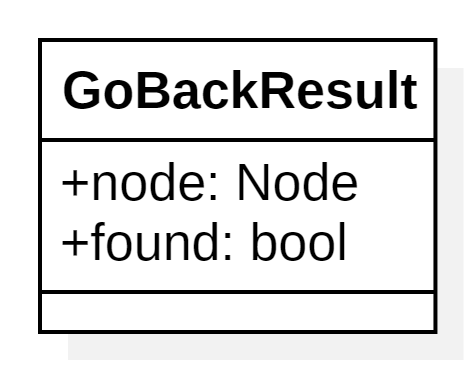
\includegraphics[width=.3\linewidth]{../../../Assets/Classi/GoBackResult.png}
                              \caption{GoBackResult: classe}
                        \end{figure}
                    \end{center}
                    
                    Value object resitutito da {\ttfamily SessionNavigator.go\_back()}. Indica se il \textit{nodo}\textsubscript{\href{https://atlasteam9.github.io/Atlas/glossario.html\#Nodo}{G}} target è stato trovato e, in caso positivo, il \textit{nodo}\textsubscript{\href{https://atlasteam9.github.io/Atlas/glossario.html\#Nodo}{G}} stesso.\\\\
                    \textbf{Attributi}
                    \begin{itemize}
                        \item {\ttfamily node: Node}: \textit{nodo}\textsubscript{\href{https://atlasteam9.github.io/Atlas/glossario.html\#Nodo}{G}} da ripetere;
                        \item {\ttfamily found: bool}: flag che indica se il \textit{nodo}\textsubscript{\href{https://atlasteam9.github.io/Atlas/glossario.html\#Nodo}{G}} era nello stack.
                    \end{itemize}    

                    
                \paragraph{SessionNavigator}\mbox{}\\

                    \begin{center}
                        \begin{figure}[H]
                              \centering
                              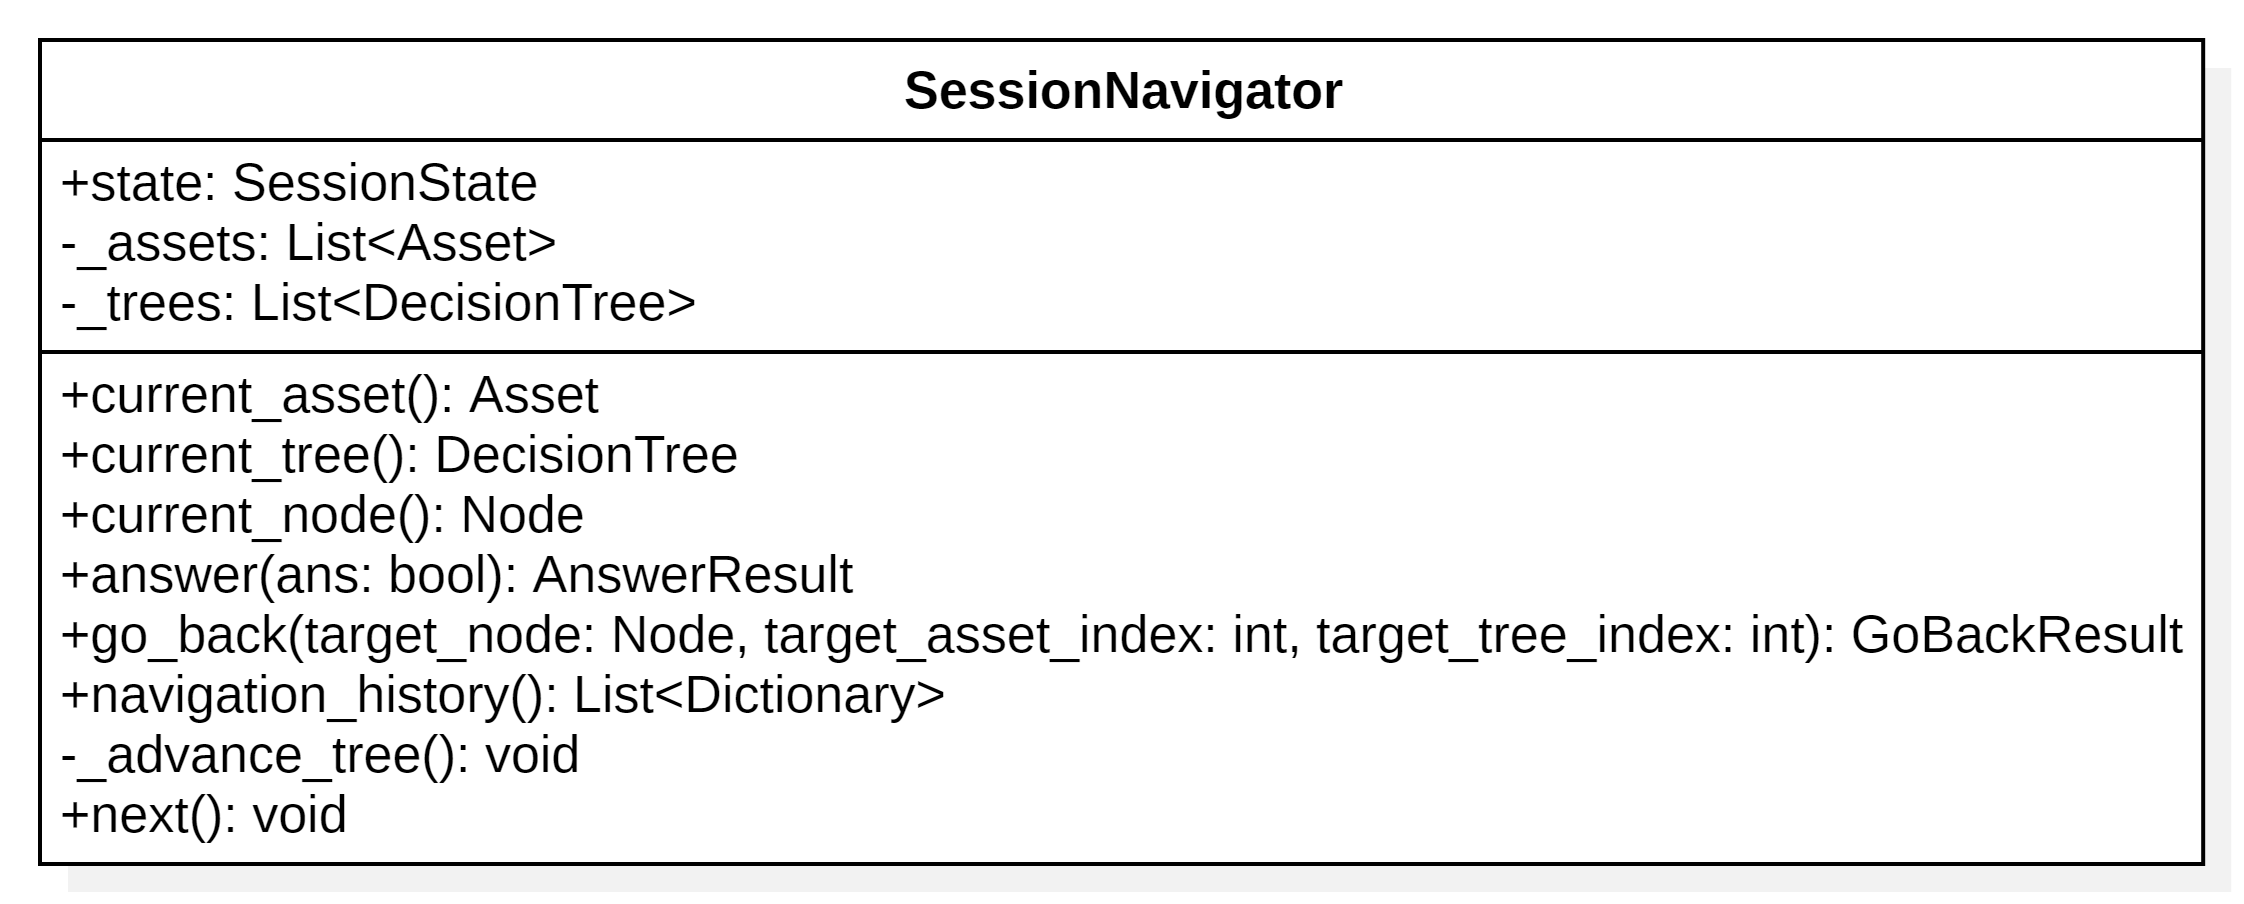
\includegraphics[width=.6\linewidth]{../../../Assets/Classi/SessionNavigator.png}
                              \caption{SessionNavigator: classe}
                        \end{figure}
                    \end{center}
                    
                    Gestisce la navigazione all'interno della sessione.\\\\
                    \textbf{Attributi}
                    \begin{itemize}
                        \item {\ttfamily state: SessionState}: stato della sessione;
                        \item {\ttfamily \_assets: list<Asset>}: \textit{lista}\textsubscript{\href{https://atlasteam9.github.io/Atlas/glossario.html\#Lista}{G}} degli asset;
                        \item {\ttfamily \_trees: list<DecisionTree>}: \textit{lista}\textsubscript{\href{https://atlasteam9.github.io/Atlas/glossario.html\#Lista}{G}} dei decision trees;
                    \end{itemize}
                    \textbf{Metodi}
                    \begin{itemize}
                        \item {\ttfamily current\_asset(): Asset}: ritorna l'asset corrente;
                        \item {\ttfamily current\_tree(): DecisionTree}: ritorna il \textit{decision tree}\textsubscript{\href{https://atlasteam9.github.io/Atlas/glossario.html\#DecisionTree}{G}} corrente;
                        \item {\ttfamily current\_node(): Node}: ritorna il \textit{nodo}\textsubscript{\href{https://atlasteam9.github.io/Atlas/glossario.html\#Nodo}{G}} corrente all'interno del tree attivo;
                        \item {\ttfamily answer(ans: bool): AnswerResult}: Processa la risposta al \textit{nodo}\textsubscript{\href{https://atlasteam9.github.io/Atlas/glossario.html\#Nodo}{G}} corrente. Se il ramo porta a un altro \textit{nodo}\textsubscript{\href{https://atlasteam9.github.io/Atlas/glossario.html\#Nodo}{G}}, aggiorna il current node e lo restituisce. Se il ramo porta a un Result, avanza al prossimo tree e restituisce il risultato da registrare;
                        \item {\ttfamily go\_back(target\_node: Node, target\_asset\_index: int, target\_tree\_index: int): GoBackResult}: torna  al \textit{nodo}\textsubscript{\href{https://atlasteam9.github.io/Atlas/glossario.html\#Nodo}{G}} target cancellando tutte le rispose successive;
                        \item {\ttfamily navigation\_history(): list<Dictionary>}: restituisce la \textit{lista}\textsubscript{\href{https://atlasteam9.github.io/Atlas/glossario.html\#Lista}{G}} dei nodi già risposti nel \textit{decision tree}\textsubscript{\href{https://atlasteam9.github.io/Atlas/glossario.html\#DecisionTree}{G}} corrente;
                        \item {\ttfamily \_advance\_tree(): void}: avanza al prossimo albero;
                        \item {\ttfamily next(): void}: metodo pubblico che richiama {\ttfamily \_advance\_tree()}.
                    \end{itemize}
                \paragraph{ResultStore}

                    \begin{center}
                        \begin{figure}[H]
                              \centering
                              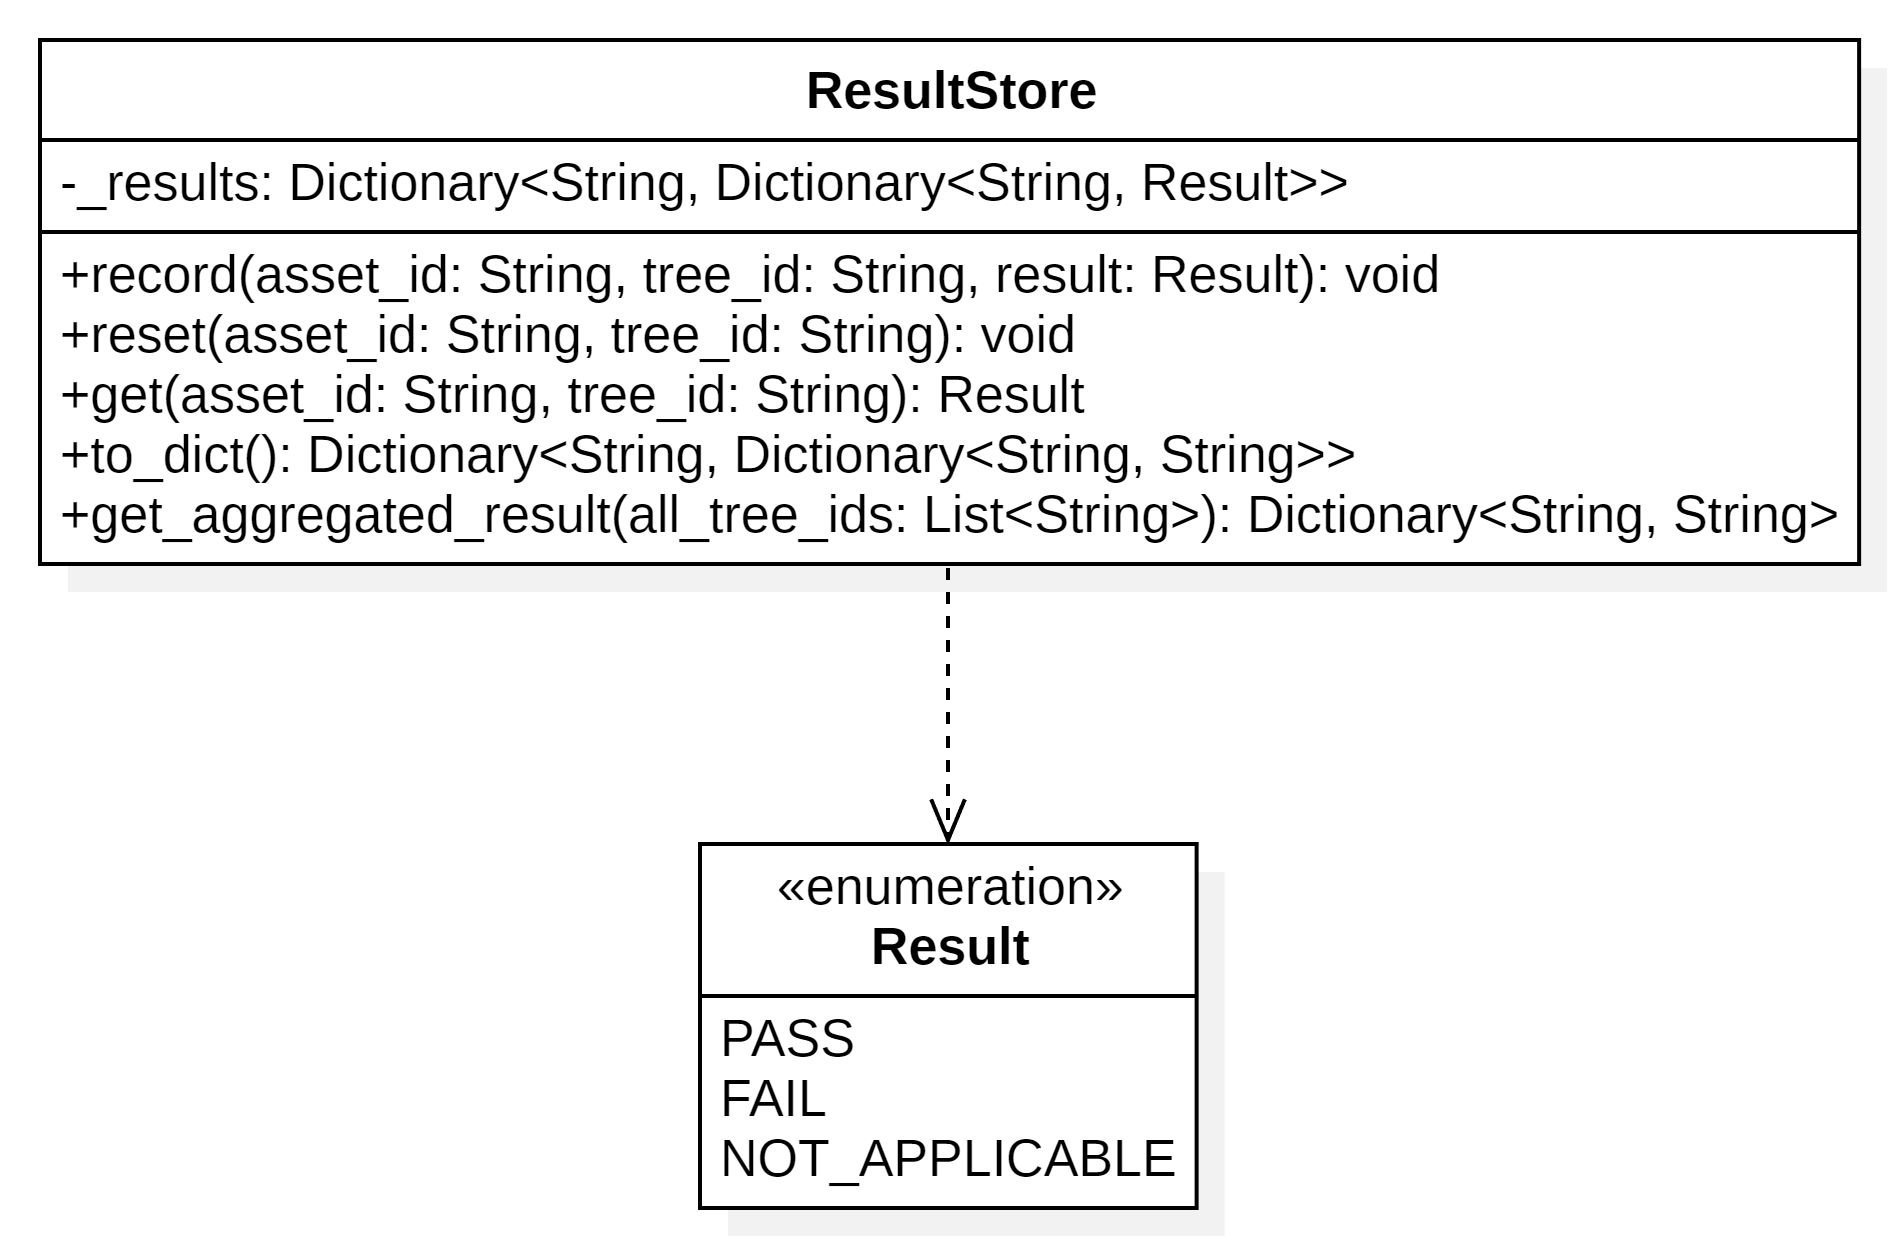
\includegraphics[width=.6\linewidth]{../../../Assets/Classi/ResultStore.png}
                              \caption{ResultStore: classe e relativa enumerazione}
                        \end{figure}
                    \end{center}
                    
                    Dizionario a due livelli che registra i risultati accumulati durante la sessione.\\\\
                    \textbf{Attributi}
                    \begin{itemize}
                        \item {\ttfamily \_results: Dictionary$<$String, Dictionary$<$String, Result$>>$}: dizionario dei risultati;
                    \end{itemize}
                    \textbf{Metodi}
                    \begin{itemize}
                        \item {\ttfamily record(asset\_id: String, tree\_id: String, result: Result): void}: registra il risultato;
                        \item {\ttfamily reset(asset\_id: String, tree\_id: String): void}: resetta il risultato sull'asset e \textit{decision tree}\textsubscript{\href{https://atlasteam9.github.io/Atlas/glossario.html\#DecisionTree}{G}} passati come parametri;
                        \item {\ttfamily get(asset\_id: String, tree\_id: String): Result}: ritorna il risultato in base all'asset e al \textit{decision tree}\textsubscript{\href{https://atlasteam9.github.io/Atlas/glossario.html\#DecisionTree}{G}};
                        \item {\ttfamily to\_dict(): Dictionary$<$String, Dictionary$<$String, String$>>$}: ritorna un dizionario con i nuovi valori??????? 
                        \item {\ttfamily get\_aggregated\_result(all\_tree\_ids: List<String>): Dictionary<String, String>}: calcola il risultato globale per ogni \textit{requisito}\textsubscript{\href{https://atlasteam9.github.io/Atlas/glossario.html\#Requisito}{G}} (albero) basandosi su tutti gli asset.
                    \end{itemize}

                \paragraph{Result}\mbox{}\\
                    Enumerazione contenente i tre possibili esiti del \textit{decision tree}\textsubscript{\href{https://atlasteam9.github.io/Atlas/glossario.html\#DecisionTree}{G}}:
                    \begin{itemize}
                        \item \textit{PASS}\textsubscript{\href{https://atlasteam9.github.io/Atlas/glossario.html\#Pass}{G}};
                        \item \textit{FAIL}\textsubscript{\href{https://atlasteam9.github.io/Atlas/glossario.html\#Fail}{G}};
                        \item NOT\_APPLICABLE.
                    \end{itemize}
                    
                \paragraph{DependencyEvaluator}\mbox{}\\

                    \begin{center}
                        \begin{figure}[H]
                              \centering
                              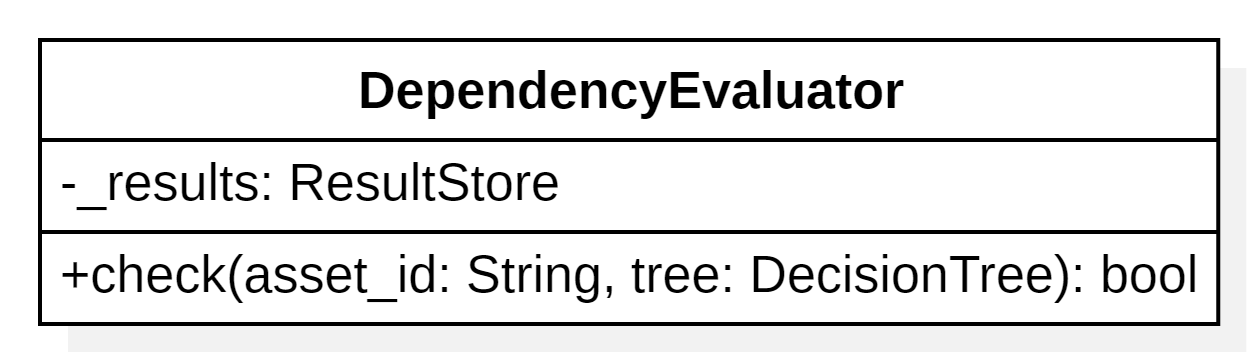
\includegraphics[width=.6\linewidth]{../../../Assets/Classi/DependencyEvaluator.png}
                              \caption{DependencyEvaluator: classe}
                        \end{figure}
                    \end{center}

                    
                    Verifica se le dipendenze di un albero sono soddisfatte per un certo asset.\\\\
                    \textbf{Attributi}
                    \begin{itemize}
                        \item {\ttfamily \_results: ResultStore}: dizionario dei risultati;
                    \end{itemize}
                    \textbf{Metodi}
                    \begin{itemize}
                        \item {\ttfamily check(asset\_id: String, tree: DecisionTree): bool}: ritorna true/false in base al rispetto/non rispetto delle dipendenze.
                    \end{itemize}  

                    \paragraph{DependencyManager}\mbox{}\\

                    \begin{center}
                        \begin{figure}[H]
                              \centering
                              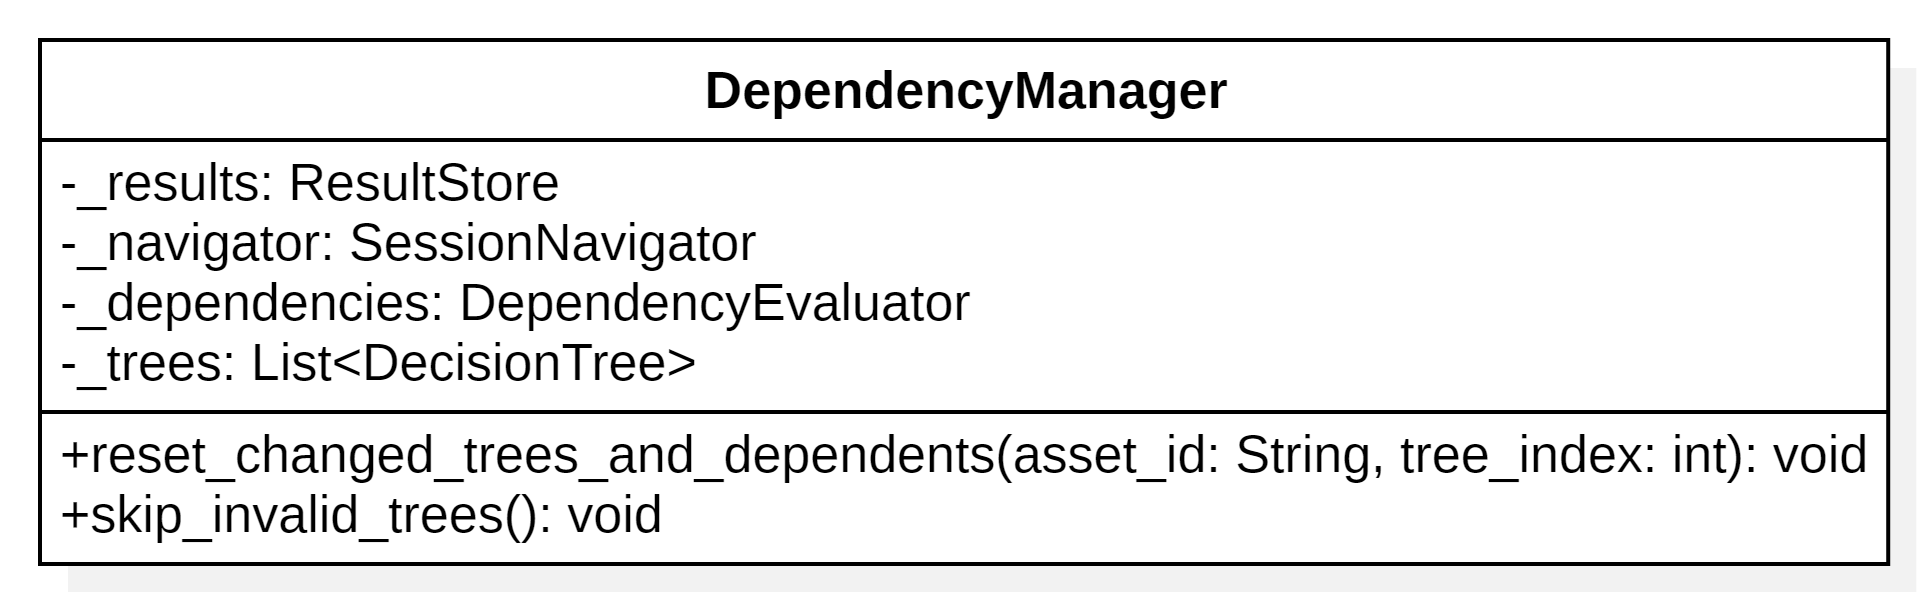
\includegraphics[width=.6\linewidth]{../../../Assets/Classi/DependencyManager.png}
                              \caption{DependencyManager: classe}
                        \end{figure}
                    \end{center}

                    
                    Gestisce le regole di dipendenza tra \textit{decision tree}\textsubscript{\href{https://atlasteam9.github.io/Atlas/glossario.html\#DecisionTree}{G}} durante la navigazione
                    e quando una risposta viene modificata.\\\\
                    \textbf{Attributi}
                    \begin{itemize}
                        \item {\ttfamily \_results: ResultStore}: dizionario dei risultati;
                        \item {\ttfamily \_navigator: SessionNavigator}: gestore della navigazione della sessione;
                        \item {\ttfamily \_dependencies: DependencyEvaluator}: \textit{verificatore}\textsubscript{\href{https://atlasteam9.github.io/Atlas/glossario.html\#Verificatore}{G}} delle dipendenze;
                        \item {\ttfamily \_trees: List<DecisionTree>}: \textit{lista}\textsubscript{\href{https://atlasteam9.github.io/Atlas/glossario.html\#Lista}{G}} dei decision tree.
                    \end{itemize}
                    \textbf{Metodi}
                    \begin{itemize}
                        \item {\ttfamily reset\_changed\_trees\_and\_dependents(asset\_id: String, tree\_index: int): void}: resetta le dipendenze in caso di modifica di una risposta ad un \textit{decision tree}\textsubscript{\href{https://atlasteam9.github.io/Atlas/glossario.html\#DecisionTree}{G}};
                        \item {\ttfamily skip\_invalid\_trees(): void}: salta gli alberi in base alle dipendenze.
                    \end{itemize}  

            
                \paragraph{SessionFactory}

                    \begin{center}
                        \begin{figure}[H]
                              \centering
                              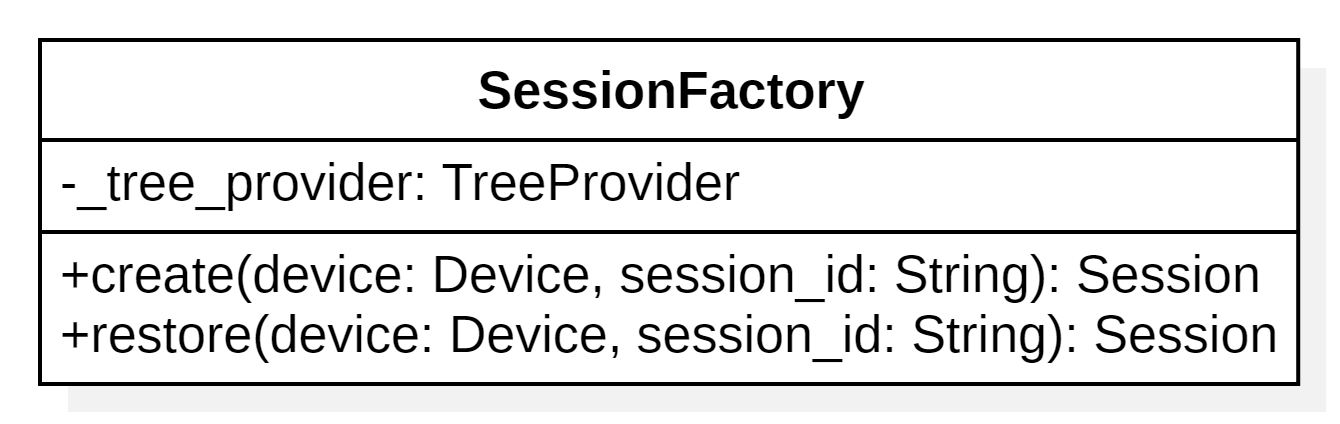
\includegraphics[width=.6\linewidth]{../../../Assets/Classi/SessionFactory.png}
                              \caption{SessionFactory: classe}
                        \end{figure}
                    \end{center}
                    
                    Centralizza la costruzione di oggetti Session.\\\\
                    \textbf{Attributi}
                    \begin{itemize}
                        \item {\ttfamily tree\_provider: TreeProvider}: dipendenza ricevuta per caricare gli alberi.
                    \end{itemize}
                    \textbf{Metodi}
                    \begin{itemize}
                        \item {\ttfamily create(device: Device, session\_id: String): Session}: genera un nuovo id e istanzia tutti i componenti interni;
                        \item {\ttfamily restore(device: Device, session\_id: String): Session}: crea una session partendo da dati già persistiti.
                    \end{itemize}

                \paragraph{DomainException}
                
                    \begin{center}
                        \begin{figure}[H]
                              \centering
                              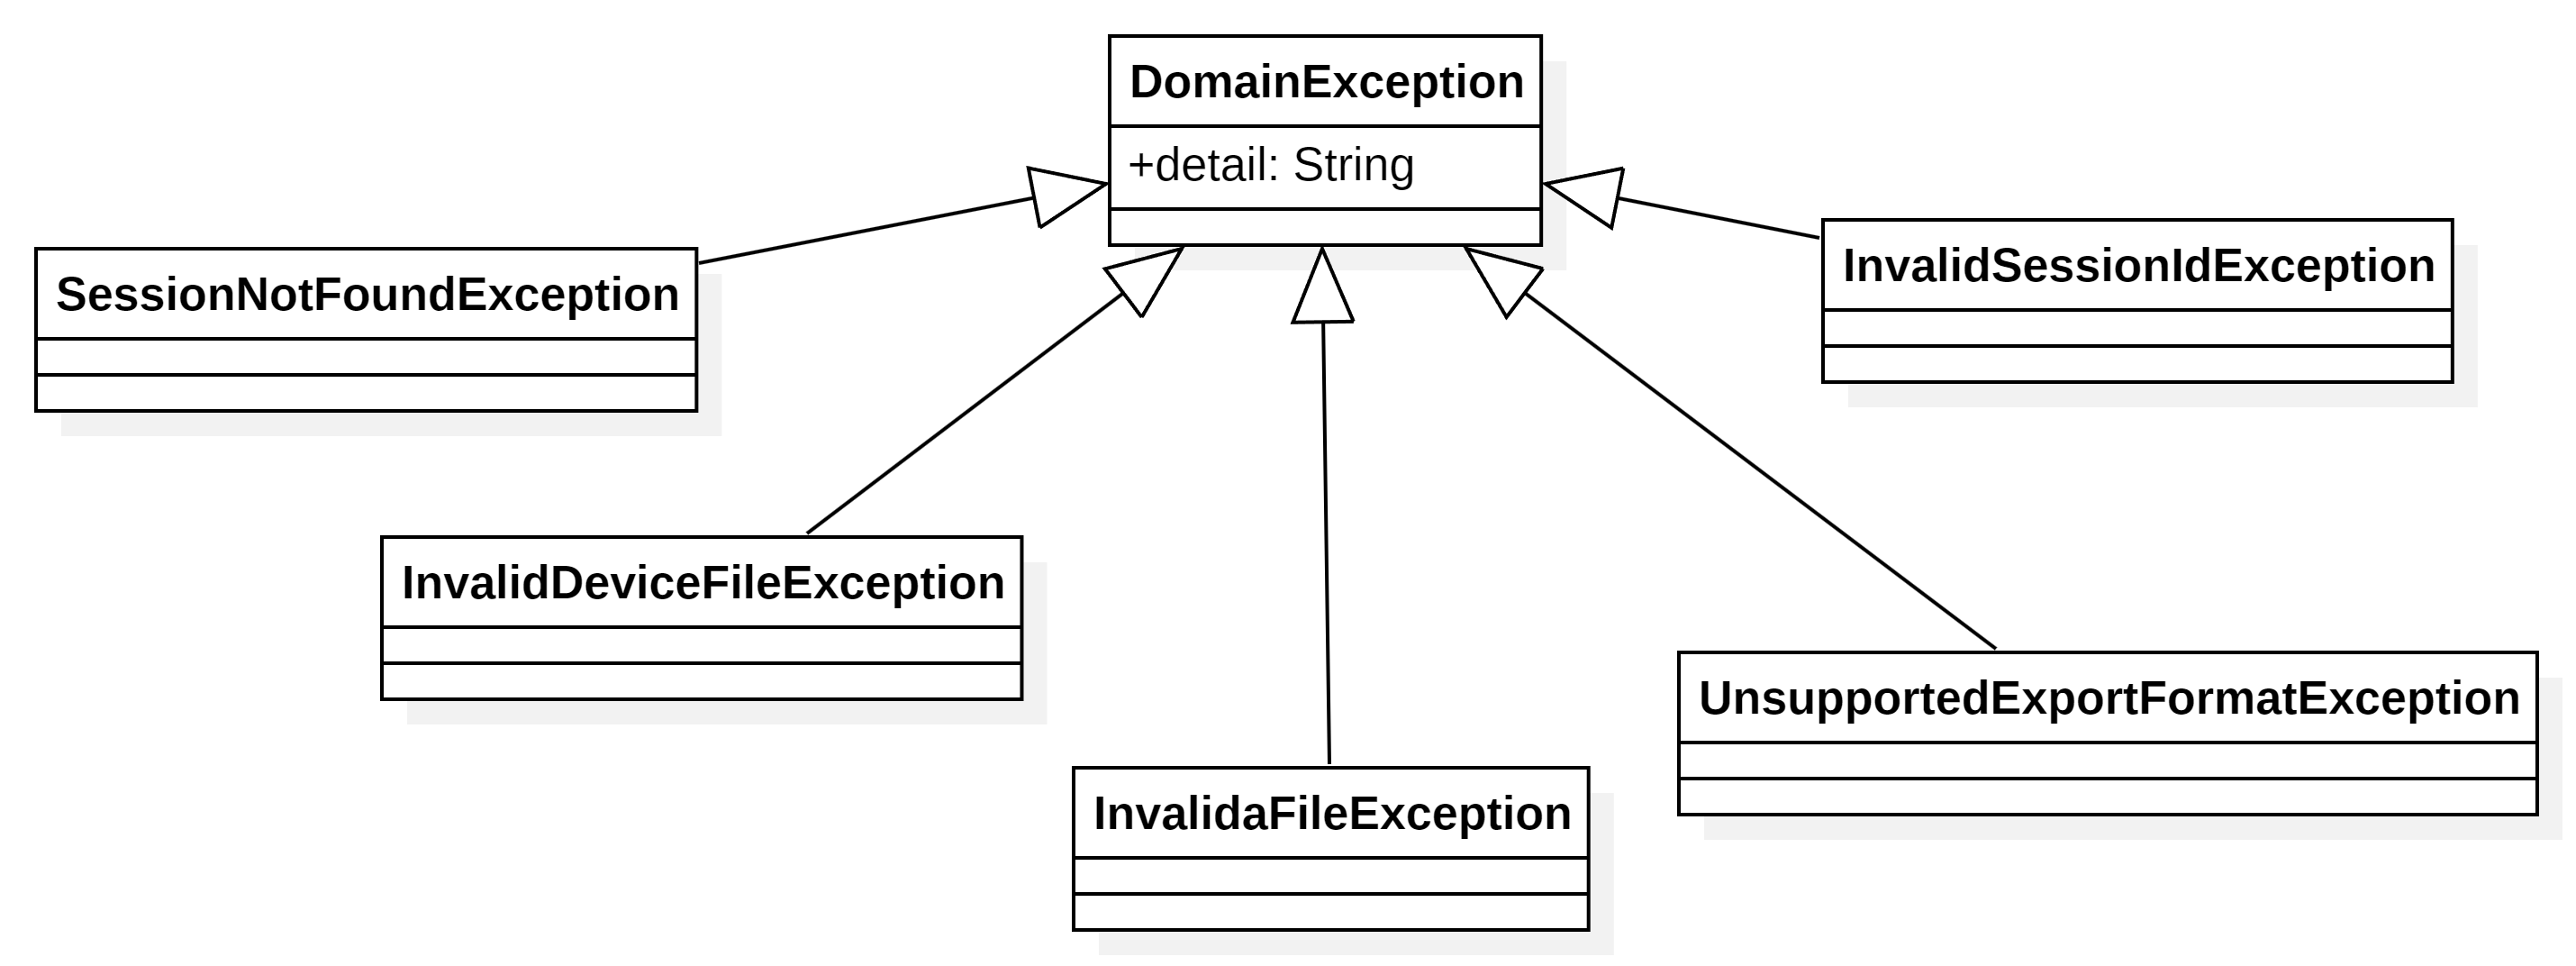
\includegraphics[width=.8\linewidth]{../../../Assets/Classi/Exceptions.png}
                              \caption{Eccezioni: classe base e derivate}
                        \end{figure}
                    \end{center}
                    
                    Classe base per tutte le eccezioni di dominio.\\\\
                    \textbf{Attributo}
                    \begin{itemize}
                        \item {\ttfamily detail: String}: messaggio leggibile.
                    \end{itemize}

                \paragraph{SessionNotFoundException}\mbox{}\\
                    Sollevata quando si cerca una sessione con un id che non esiste né in cache né nel repository.

                \paragraph{InvalidDeviceFileException}\mbox{}\\
                    Sollevata quando il file json del device non supera la \textit{validazione}\textsubscript{\href{https://atlasteam9.github.io/Atlas/glossario.html\#Validazione}{G}} dello schema Pydantic.

                \paragraph{InvalidFileException}\mbox{}\\
                    Sollevata quando ????.

                \paragraph{UnsupportedExportFormatException}\mbox{}\\
                    Sollevata quando il formato richiesto per l'export non è tra quelli disponibili (\textit{csv}\textsubscript{\href{https://atlasteam9.github.io/Atlas/glossario.html\#CSV}{G}}, \textit{pdf}\textsubscript{\href{https://atlasteam9.github.io/Atlas/glossario.html\#PDF}{G}}).

                \paragraph{InvalidSessionIdException}\mbox{}\\
                    Sollevata quando session\_id fornito in una richiesta non è un UUID v4 valido.
                    

                \paragraph{ExportStrategy}\mbox{}\\

                    \begin{center}
                        \begin{figure}[H]
                            \centering
                            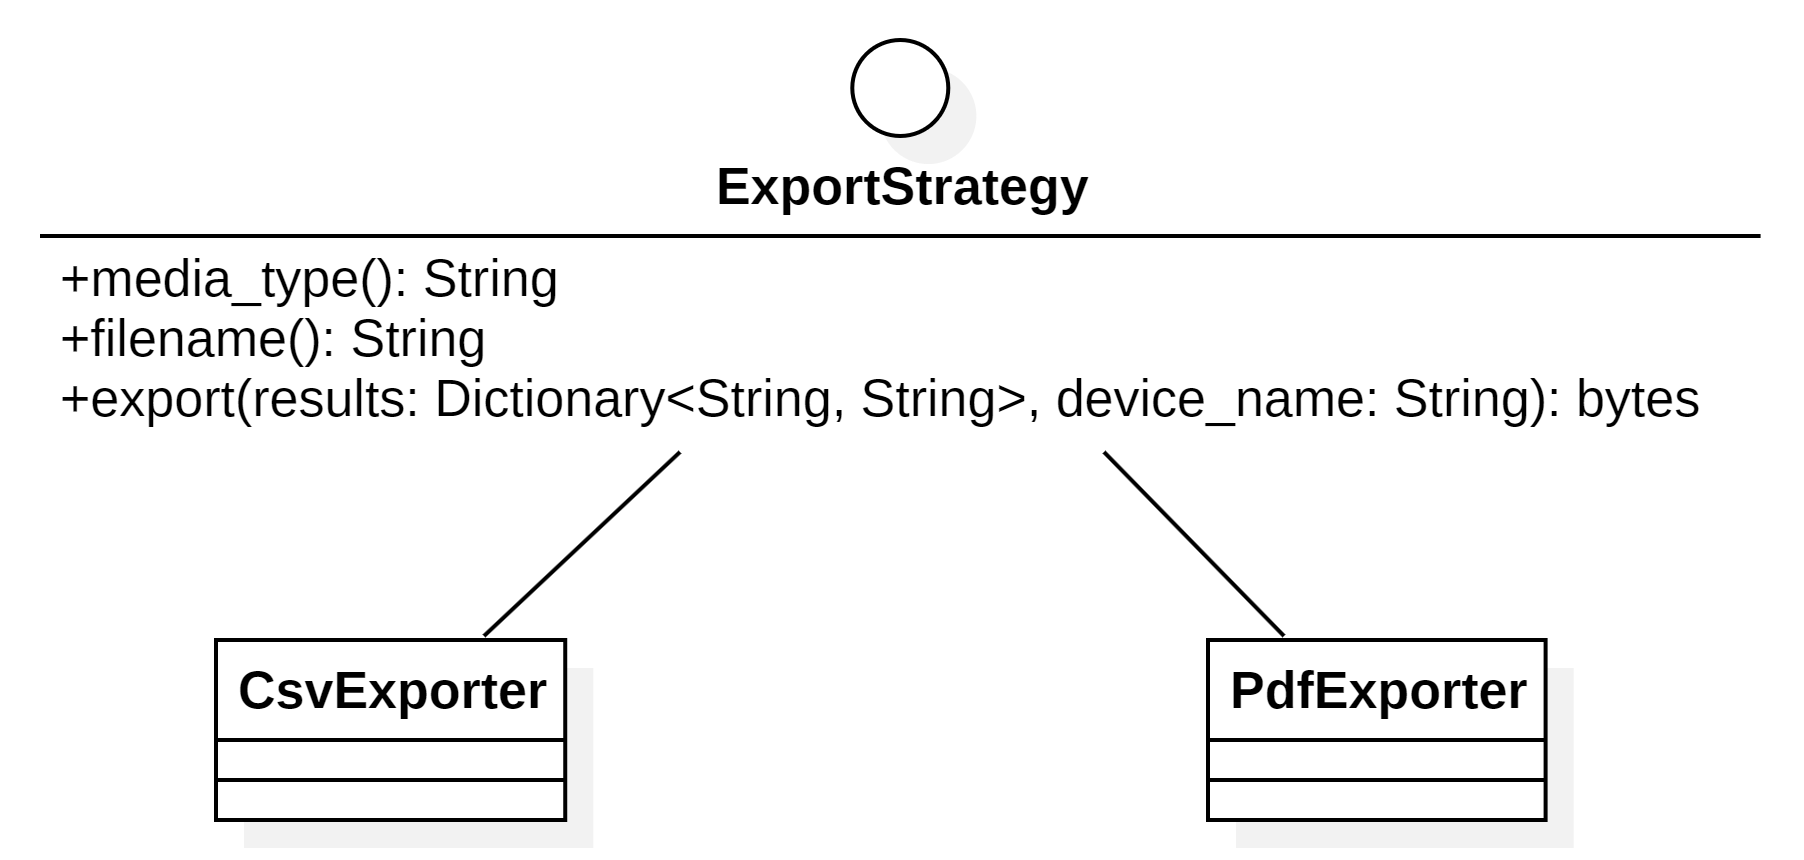
\includegraphics[width=.6\linewidth]{../../../Assets/Classi/Exporters.png}
                            \caption{Esportatori: interfaccia e classi}
                        \end{figure}
                    \end{center}

                    \textit{Interfaccia}\textsubscript{\href{https://atlasteam9.github.io/Atlas/glossario.html\#Interfaccia}{G}} utilizzata per definire il contratto per le strategie di \textit{esportazione}\textsubscript{\href{https://atlasteam9.github.io/Atlas/glossario.html\#Esportazione}{G}} dei risultati.\\\\
                    \textbf{Metodi}
                    \begin{itemize}
                        \item {\ttfamily media\_type(): String}: definisce il tipo di file;
                        \item {\ttfamily filename(): String}: definisce il nome del file;
                        \item {\ttfamily export(results: Dictionary$<$String, Dictionary$<$String, String$>>$, device\_name: String): bytes}: riceve il dizionario dei risultati, il nome del device e restituisce i byte del file del prodotto.
                    \end{itemize}
                
                \paragraph{CsvExporter}\mbox{}\\
                    Implementa ExportStrategy producendo un file \textit{CSV}\textsubscript{\href{https://atlasteam9.github.io/Atlas/glossario.html\#CSV}{G}} con colonne Device, AssetID, TreeID, Result e una coppia (asset, albero) per ogni riga con il rispettivo risultato.\\\\
                    \textbf{Metodi}
                    \begin{itemize}
                        \item Implementazione dei metodi {\ttfamily media\_type()}, {\ttfamily filename()} ed {\ttfamily export()} definiti dall'\textit{interfaccia}\textsubscript{\href{https://atlasteam9.github.io/Atlas/glossario.html\#Interfaccia}{G}} ExportStrategy.
                    \end{itemize}

                \paragraph{PdfExporter}\mbox{}\\
                    Implementa ExportStrategy producendo un file \textit{PDF}\textsubscript{\href{https://atlasteam9.github.io/Atlas/glossario.html\#PDF}{G}} formattato con ReportLab. Per ogni asset genera una tabella con intestazione colorata, righe alternate e colorazione del testo del risultato (verde per \textit{PASS}\textsubscript{\href{https://atlasteam9.github.io/Atlas/glossario.html\#Pass}{G}}, rosso per \textit{FAIL}\textsubscript{\href{https://atlasteam9.github.io/Atlas/glossario.html\#Fail}{G}} e grigio per NOT\_APPLICABLE)\\\\
                    \textbf{Metodi}
                    \begin{itemize}
                        \item Implementazione dei metodi {\ttfamily media\_type()}, {\ttfamily filename()} ed {\ttfamily export()} definiti dall'\textit{interfaccia}\textsubscript{\href{https://atlasteam9.github.io/Atlas/glossario.html\#Interfaccia}{G}} ExportStrategy.
                    \end{itemize}   
                    

            \subsubsection{Infrastructure Layer}

                \paragraph{FileStorage}\mbox{}\\

                    \begin{center}
                        \begin{figure}[H]
                              \centering
                              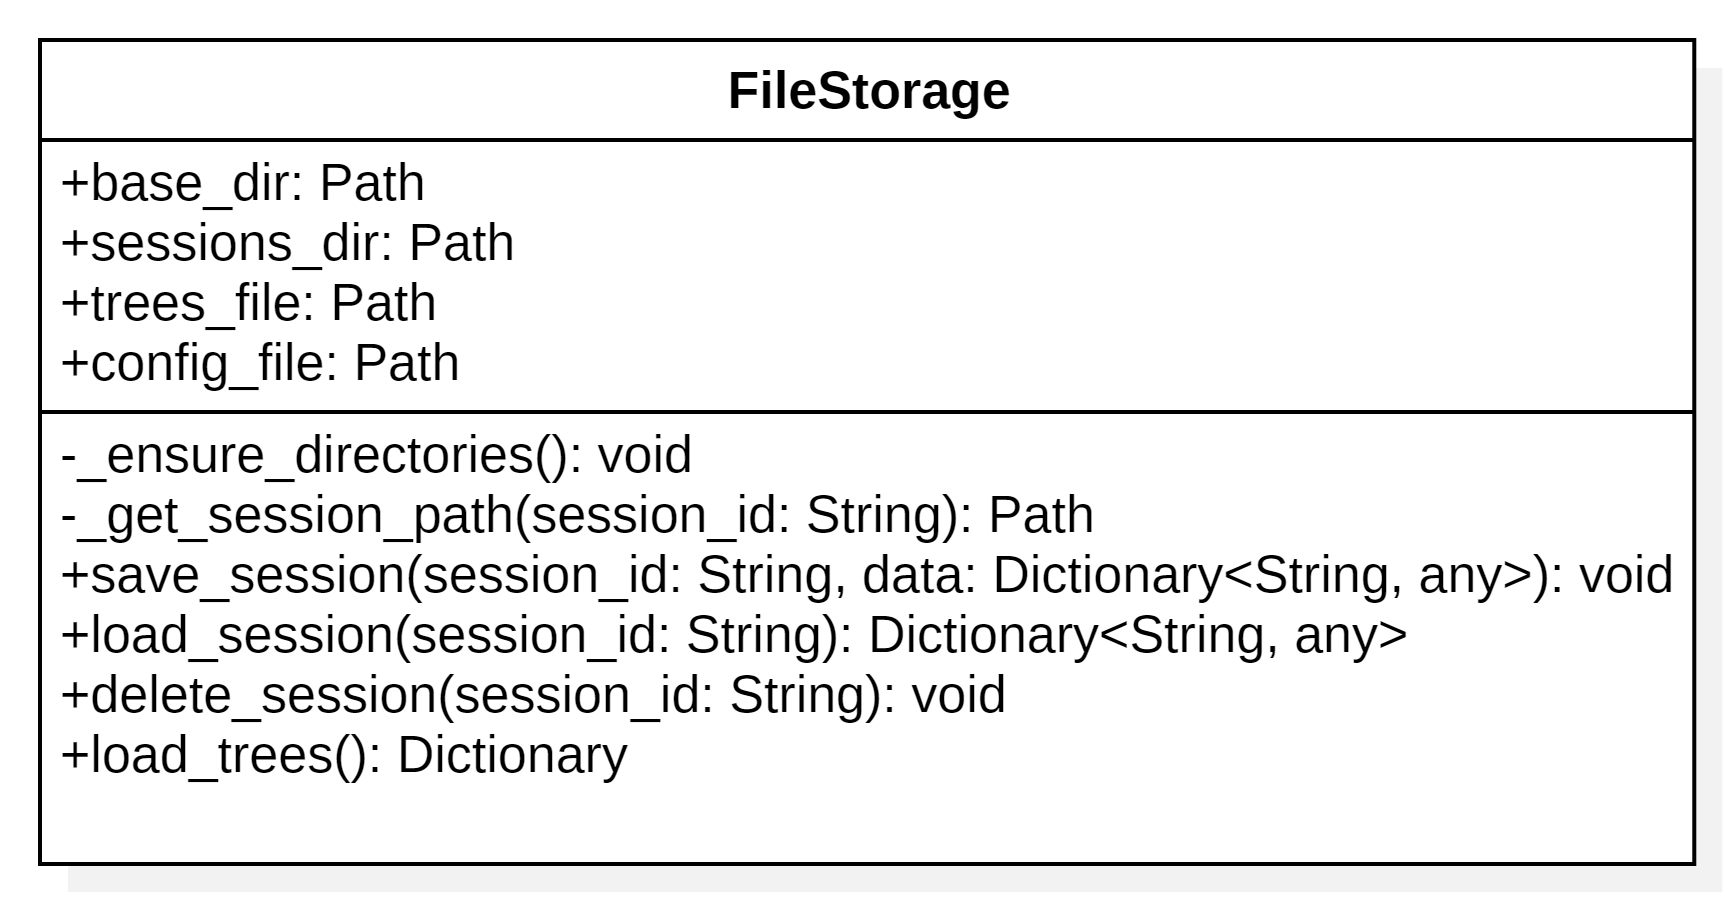
\includegraphics[width=.6\linewidth]{../../../Assets/Classi/FileStorage.png}
                              \caption{FileStorage: classe}
                        \end{figure}
                    \end{center}
                
                    Gestisce le operazioni di I/O su disco. Crea e mantiene la struttura di directory (data/sessions/).\\\\
                    \textbf{Attributi}
                    \begin{itemize}
                        \item {\ttfamily base\_dir: Path}: directory base;
                        \item {\ttfamily session\_dir: Path}: directory delle sessioni;
                        \item {\ttfamily trees\_file: Path}: file contenente i decision trees;
                        \item {\ttfamily config\_file: Path}: file di configurazione.
                    \end{itemize}
                    \textbf{Metodi}
                    \begin{itemize}
                        \item {\ttfamily \_ensure\_directories: void}: assicura che le directory esistano. Se queste non esistono, vengono create;
                        \item {\ttfamily \_get\_session\_path(session\_id: String): Path}: ritorna il Path di una sessione salvata;
                        \item {\ttfamily save\_session(session\_id: String, data: Dictionary<String, any>): void}: salva la sessione su file. Il salvataggio avviene prima effettuando una scrittura su file .tmp, eseguendo poi un rename per evitare file corrotti in caso di crash;
                        \item {\ttfamily load\_session(session\_id: String): Dictionary<String, any>}: carica la sessione da file;
                        \item {\ttfamily delete\_session(session\_id: String): void}: elimina il file contenente la sessione passata per parametro;
                        \item {\ttfamily load\_trees(): Dictionary}: carica i decision trees dal file json.
                    \end{itemize}


                \paragraph{TreeProvider}

                    \begin{center}
                        \begin{figure}[H]
                              \centering
                              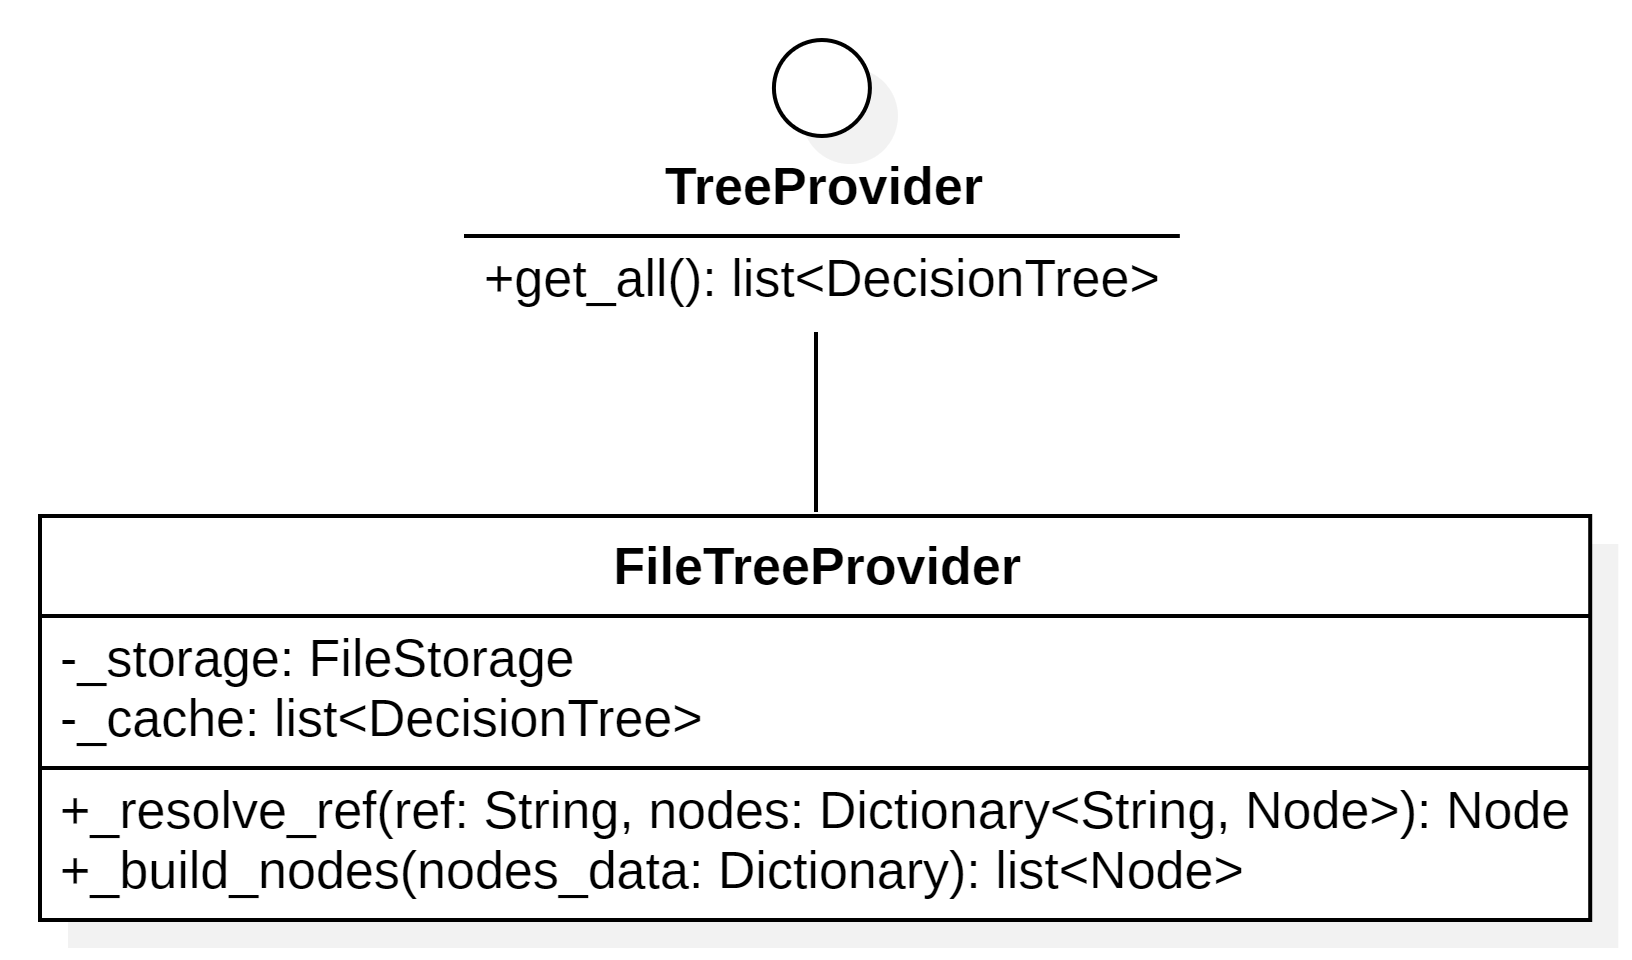
\includegraphics[width=.6\linewidth]{../../../Assets/Classi/TreeProvider.png}
                              \caption{TreeProvider: interfaccia e classe}
                        \end{figure}
                    \end{center}
                
                    \textit{Interfaccia}\textsubscript{\href{https://atlasteam9.github.io/Atlas/glossario.html\#Interfaccia}{G}} utilizzata per disaccoppiare il dominio dalla sorgente concreta degli alberi.\\\\
                    \textbf{Metodi}
                    \begin{itemize}
                        \item {\ttfamily get\_all(): list<DecisionTree>}: ritorna la \textit{lista}\textsubscript{\href{https://atlasteam9.github.io/Atlas/glossario.html\#Lista}{G}} completa dei decision tree.
                    \end{itemize}
                
                \paragraph{FileTreeProvider}\mbox{}\\
                    Implementa l'\textit{interfaccia}\textsubscript{\href{https://atlasteam9.github.io/Atlas/glossario.html\#Interfaccia}{G}} TreeProvider, leggendo gli alberi da \textit{trees.json} tramite FileStorage.\\\\
                    \textbf{Attributi}
                        \begin{itemize}
                            \item {\ttfamily \_storage: FileStorage}: gestore delle operazioni di I/O;
                            \item {\ttfamily \_cache: list<DecisionTree>}: cache lazy, caricata alla prima chiamata;
                        \end{itemize}
                    \textbf{Metodi}
                    \begin{itemize}
                        \item {\ttfamily \_resolve\_ref(ref: String, nodes: Dictionary<String, Node>): Node | Result}: risolve i riferimenti a nodi successivi e risultati foglia?????????????????????;
                        \item {\ttfamily build\_nodes(nodes\_data: Dictionary): list<Node>}: costruisce ricorsivamente la struttura Node dal json;
                        \item {\ttfamily get\_all(): list<DecisionTree>}: implementazione del metodo dichiarato nell'\textit{interfaccia}\textsubscript{\href{https://atlasteam9.github.io/Atlas/glossario.html\#Interfaccia}{G}} TreeProvider;
                    \end{itemize}

                \paragraph{BaseRepository}

                    \begin{center}
                        \begin{figure}[H]
                              \centering
                              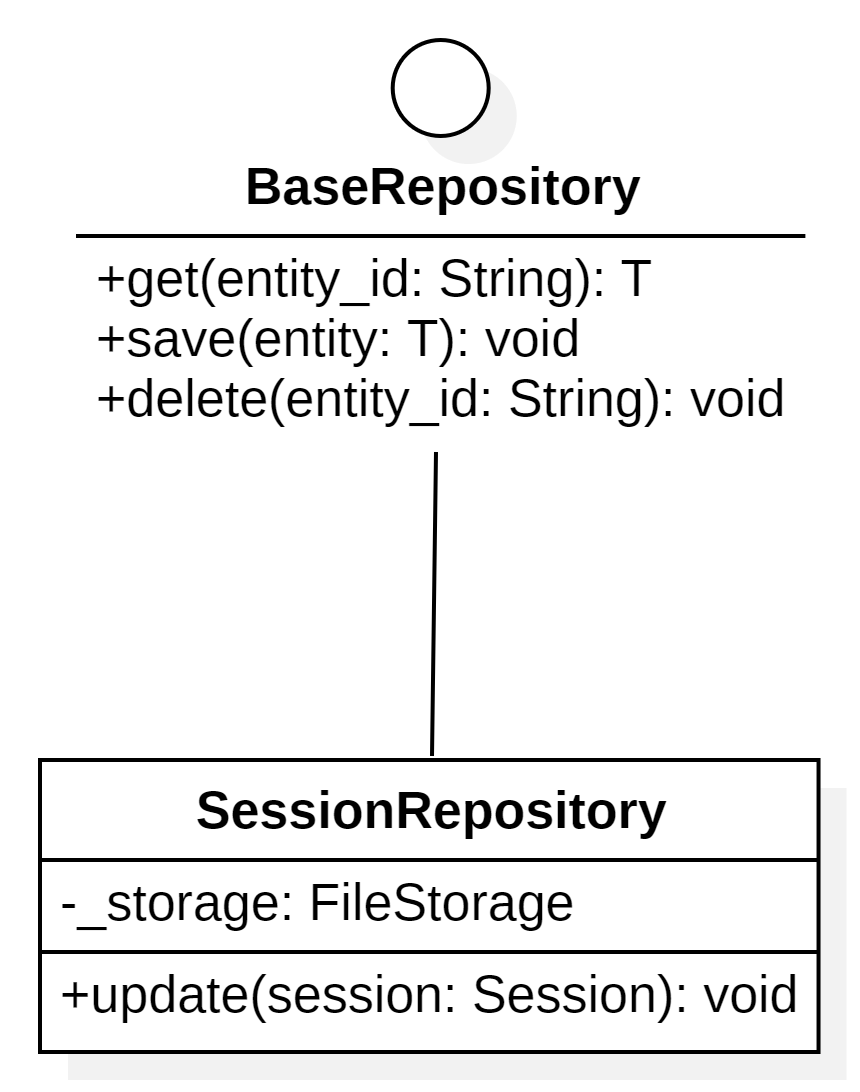
\includegraphics[width=.4\linewidth]{../../../Assets/Classi/BaseRepository.png}
                              \caption{BaseRepository: interfaccia e classe}
                        \end{figure}
                    \end{center}
                
                    \textit{Interfaccia}\textsubscript{\href{https://atlasteam9.github.io/Atlas/glossario.html\#Interfaccia}{G}} generica astratta per il pattern repository.\\\\
                    \textbf{Metodi}
                    \begin{itemize}
                        \item {\ttfamily save(\textit{entity}\textsubscript{\href{https://atlasteam9.github.io/Atlas/glossario.html\#Entity}{G}}: T): void}: salva un'entità nel \textit{repository}\textsubscript{\href{https://atlasteam9.github.io/Atlas/glossario.html\#Repository}{G}};
                        \item {\ttfamily get(\textit{entity}\textsubscript{\href{https://atlasteam9.github.io/Atlas/glossario.html\#Entity}{G}}\_id: String): T}: recupera un'entità dal \textit{repository}\textsubscript{\href{https://atlasteam9.github.io/Atlas/glossario.html\#Repository}{G}};
                        \item {\ttfamily delete(\textit{entity}\textsubscript{\href{https://atlasteam9.github.io/Atlas/glossario.html\#Entity}{G}}\_id: String): void}: elimina un'entità dal repository.
                    \end{itemize}
                    
                \paragraph{SessionRepository}\mbox{}\\
                    Implementa BaseRepository per le sessioni.\\\\
                    \textbf{Attributi}
                    \begin{itemize}
                        \item {\ttfamily storage: FileStorage}: gestore delle operazioni I/O;
                    \end{itemize}
                    \textbf{Metodi}
                    \begin{itemize}
                        \item {\ttfamily save(), get(), delete()}: metodi definiti dall'\textit{interfaccia}\textsubscript{\href{https://atlasteam9.github.io/Atlas/glossario.html\#Interfaccia}{G}} BaseRepository, vengono implementati;
                        \item {\ttfamily update(session: Session): void}: effettua un salvataggio della sessione.
                    \end{itemize}

        \subsection{Design Pattern utilizzati}
            In Python, sono stati utilizzati diversi \textit{design pattern}\textsubscript{\href{https://atlasteam9.github.io/Atlas/glossario.html\#DesignPattern}{G}} per aumentare la manutenibilità del software:
            \begin{itemize}
                \item \textbf{Strategy pattern}: utilizzato per la gestione dell'\textit{esportazione}\textsubscript{\href{https://atlasteam9.github.io/Atlas/glossario.html\#Esportazione}{G}} dei risultati dei test. È stata definita un'\textit{interfaccia}\textsubscript{\href{https://atlasteam9.github.io/Atlas/glossario.html\#Interfaccia}{G}} che stabilisce il contratto per 
                    l'\textit{esportazione}\textsubscript{\href{https://atlasteam9.github.io/Atlas/glossario.html\#Esportazione}{G}}, mentre implementazioni concrete forniscono il supporto per i due formati decisi (\textit{PDF}\textsubscript{\href{https://atlasteam9.github.io/Atlas/glossario.html\#PDF}{G}}, \textit{CSV}\textsubscript{\href{https://atlasteam9.github.io/Atlas/glossario.html\#CSV}{G}}). Questo approccio consente di incapsulare algoritmi intercambiabili, 
                    favorendo l'\textit{estensione}\textsubscript{\href{https://atlasteam9.github.io/Atlas/glossario.html\#Estensione}{G}} del sistema senza modificare il codice esistente e migliorando la separazione delle responsabilità;
                \item \textbf{Repository pattern}: utilizzato per astrarre la logica di accesso ai dati dalla business logic. BaseRepository definisce l'\textit{interfaccia}\textsubscript{\href{https://atlasteam9.github.io/Atlas/glossario.html\#Interfaccia}{G}} astratta generica con i metodi 
                    {\ttfamily save(), get()} e {\ttfamily delete()}, parametrizzata con TypeVar. SessionRepository è l'implementazione concreta che implementa BaseRepository, nasconde completamente i 
                    dettagli del file system e delega le operazione di I/O a FileStorage. Chi usa il \textit{repository}\textsubscript{\href{https://atlasteam9.github.io/Atlas/glossario.html\#Repository}{G}} non sa se i dati stanno su file, database o altro;
                \item \textbf{Factory pattern}: utilizzato perché l'oggetto Session è complesso da costruire, in quanto richiede l'istanziazione coordinata di diversi componenti interni.
                    La classe SessionFactory incapsula questa logica di creazione, nascondendone i dettagli al client e semplificando l'uso del sistema: il client può ottenere un'istanza di Session 
                    semplicemente invocando il metodo {\ttfamily create()};
                \item \textbf{Facade pattern}: utilizzato nella gestione della Session. La classe Session infatti non gestisce direttamente nessuna logica, ma espone un'\textit{interfaccia}\textsubscript{\href{https://atlasteam9.github.io/Atlas/glossario.html\#Interfaccia}{G}} unificata e 
                    semplificata verso l'esterno nascondendo la complessità interna dei suoi componenti (SessionNavigator, SessionState, ResultStore, DependencyEvaluator). Il chiamante usa {\ttfamily session.answer()}
                    senza sapere che internamente vengono coinvolti tutti i componenti sopracitati.
            \end{itemize}
                    
    \end{document}        